\pdfminorversion=4 % for acroread
\ifdefined\ishandout
  \documentclass[aspectratio=169,t,handout,xcolor={usenames,dvipsnames}]{beamer}
\else
  \documentclass[aspectratio=169,t,xcolor={usenames,dvipsnames}]{beamer}


\usepackage{beamerstyle}
\usepackage{dsfont}
\usepackage{bm}
\usepackage[english]{babel}
\usepackage[utf8]{inputenc}
\usepackage{graphicx}
\usepackage{algorithm}
\usepackage[ruled,vlined,algo2e,linesnumbered]{algorithm2e}
%\usepackage[boxed,vlined]{algorithm2e}
\usepackage{hyperref}
\usepackage{booktabs}
\usepackage{mathtools}
\usepackage{multimedia}

\usepackage{amsmath,amssymb}
\usepackage{listings}
\lstset{frame=lines,framesep=3pt,numbers=left,numberblanklines=false,basicstyle=\ttfamily\small}

\usepackage{subfig}
\usepackage{multicol}
%\usepackage{appendixnumberbeamer}
%
\usepackage{tcolorbox}

\usepackage{pgfplots}
\usepackage{tikz}
\usetikzlibrary{trees} 
\usetikzlibrary{shapes.geometric}
\usetikzlibrary{positioning,shapes,shadows,arrows,calc,mindmap}
\usetikzlibrary{positioning,fadings,through}
\usetikzlibrary{decorations.pathreplacing}
\usetikzlibrary{intersections}
\usetikzlibrary{positioning,fit,calc,shadows,backgrounds}
\pgfdeclarelayer{background}
\pgfdeclarelayer{foreground}
\pgfsetlayers{background,main,foreground}
\tikzstyle{activity}=[rectangle, draw=black, rounded corners, text centered, text width=8em]
\tikzstyle{data}=[rectangle, draw=black, text centered, text width=8em]
\tikzstyle{myarrow}=[->, thick, draw=black]

% Define the layers to draw the diagram
\pgfdeclarelayer{background}
\pgfdeclarelayer{foreground}
\pgfsetlayers{background,main,foreground}

%\usepackage{listings}
%\lstset{numbers=left,
%  showstringspaces=false,
%  frame={tb},
%  captionpos=b,
%  lineskip=0pt,
%  basicstyle=\ttfamily,
%%  extendedchars=true,
%  stepnumber=1,
%  numberstyle=\small,
%  xleftmargin=1em,
%  breaklines
%}

 
\definecolor{blue}{RGB}{0, 74, 153}

\usetheme{Boadilla}
%\useinnertheme{rectangles}
\usecolortheme{whale}
\setbeamercolor{alerted text}{fg=blue}
\useoutertheme{infolines}
\setbeamertemplate{navigation symbols}{\vspace{-5pt}} % to lower the logo
\setbeamercolor{date in head/foot}{bg=white} % blue
\setbeamercolor{date in head/foot}{fg=white}
\setbeamercolor{author  in head/foot}{bg=white} %blue
\setbeamercolor{title in head/foot}{bg=white} % blue
\setbeamercolor{title}{fg=white, bg=blue}
\setbeamercolor{block title}{fg=white,bg=blue}
\setbeamercolor{block body}{bg=blue!10}
\setbeamercolor{frametitle}{fg=white, bg=blue}
\setbeamercovered{invisible}

\makeatletter
\setbeamertemplate{footline}
{
  \leavevmode%
  \hbox{%
  \begin{beamercolorbox}[wd=.333333\paperwidth,ht=2.25ex,dp=1ex,center]{author in head/foot}%
%    \usebeamerfont{author in head/foot}\insertshortauthor
  \end{beamercolorbox}%
  \begin{beamercolorbox}[wd=.333333\paperwidth,ht=2.25ex,dp=1ex,center]{title in head/foot}%
    \usebeamerfont{title in head/foot}\insertshorttitle
  \end{beamercolorbox}%
  \begin{beamercolorbox}[wd=.333333\paperwidth,ht=2.25ex,dp=1ex,right]{date in head/foot}%
    \usebeamerfont{date in head/foot}\insertshortdate{}\hspace*{2em}
%    \insertframenumber\hspace*{2ex} 
  \end{beamercolorbox}}%
  \vskip0pt%
}
\makeatother

%\pgfdeclareimage[height=1.2cm]{automl}{images/logos/automl.png}
%\pgfdeclareimage[height=1.2cm]{freiburg}{images/logos/freiburg}

%\logo{\pgfuseimage{freiburg}}

\renewcommand{\comment}[1]{
	\noindent
	%\vspace{0.25cm}
	{\color{red}{\textbf{TODO:} #1}}
	%\vspace{0.25cm}
}
\newcommand{\notefh}[1]{\textcolor{red}{\textbf{FH:} #1}}
\renewcommand{\comment}[1]{}
\newcommand{\hide}[1]{}
\newcommand{\cemph}[2]{\emph{\textcolor{#1}{#2}}}

\newcommand{\lit}[1]{{\footnotesize\color{black!60}[#1]}}

\newcommand{\litw}[1]{{\footnotesize\color{blue!20}[#1]}}


\newcommand{\myframe}[2]{\begin{frame}[c]{#1}#2\end{frame}}
\newcommand{\myframetop}[2]{\begin{frame}{#1}#2\end{frame}}
\newcommand{\myit}[1]{\begin{itemize}#1\end{itemize}}
\newcommand{\myblock}[2]{\begin{block}{#1}#2\end{block}}


\newcommand{\votepurple}[1]{\textcolor{Purple}{$\bigstar$}}
\newcommand{\voteyellow}[1]{\textcolor{Goldenrod}{$\bigstar$}}
\newcommand{\voteblue}[1]{\textcolor{RoyalBlue}{$\bigstar$}}
\newcommand{\votepink}[1]{\textcolor{Pink}{$\bigstar$}}

\newcommand{\diff}{\mathop{}\!\mathrm{d}}
\newcommand{\refstyle}[1]{{\small{\textcolor{gray}{#1}}}}
\newcommand{\hands}[0]{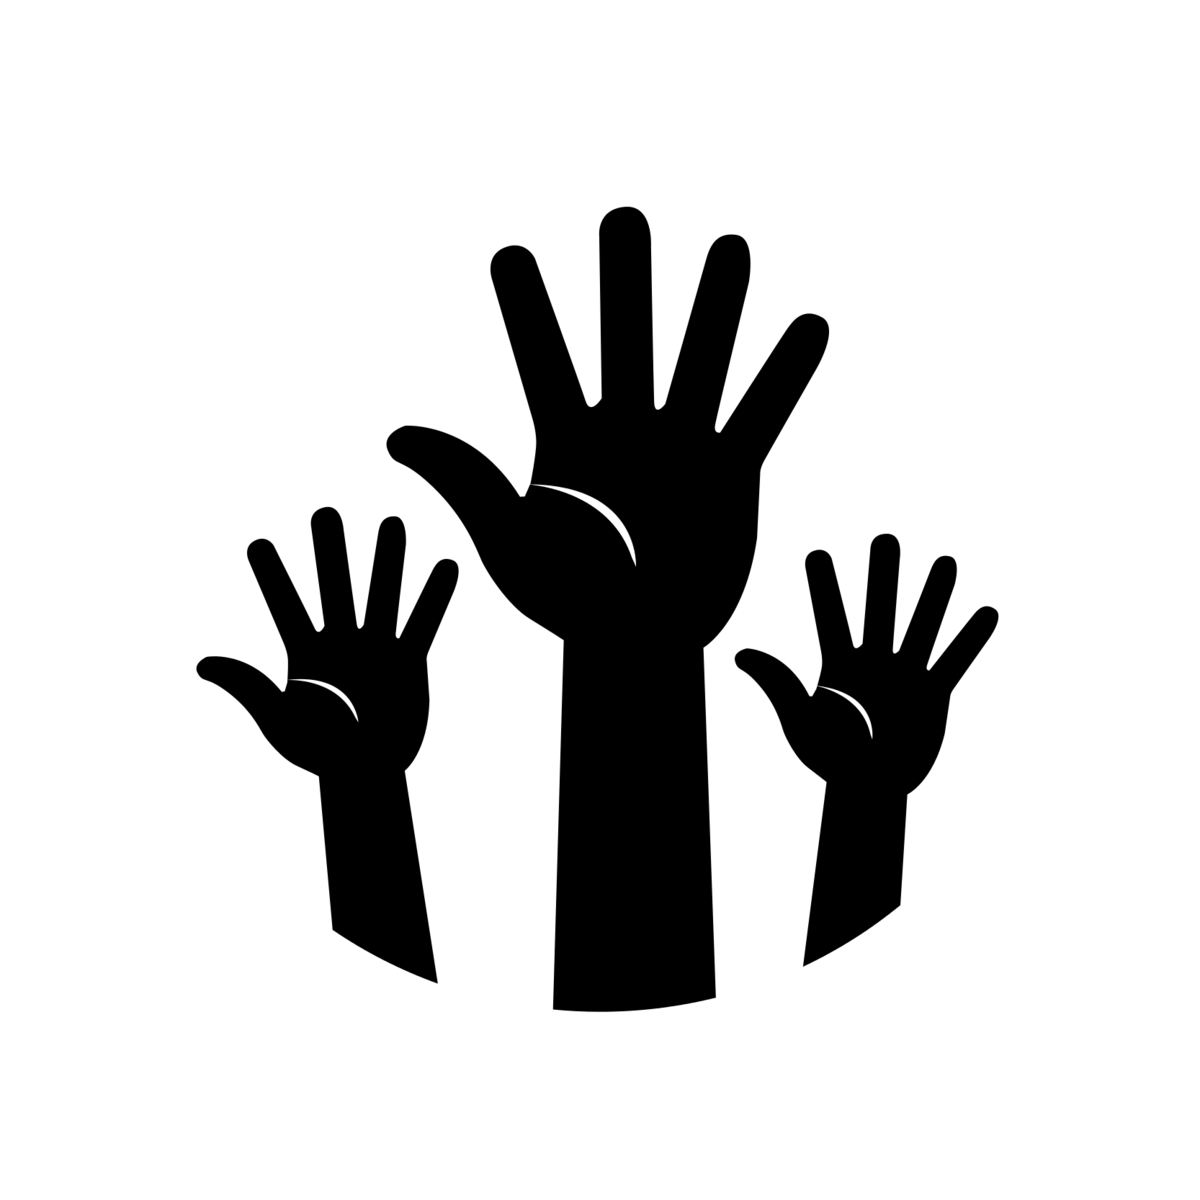
\includegraphics[height=1.5em]{images/hands}}
\newcommand{\transpose}[0]{{\textrm{\tiny{\sf{T}}}}}
\newcommand{\norm}{{\mathcal{N}}}
\newcommand{\cutoff}[0]{\kappa}
\newcommand{\instD}[0]{\dataset}
\newcommand{\insts}[0]{\mathcal{I}}
\newcommand{\inst}[0]{i}
\newcommand{\instI}[1]{i^{(#1)}}

% Iteration specific instance of variable/function/anything
% Introduced in the BO section, but moved up here to make it available within other macros
\newcommand{\iter}[2][\bocount]{{#2}^{(#1)}}

%--------HPO parameter macros-----------

% Parameter Configuration Space
\newcommand{\pcs}[0]{\pmb{\Lambda}}

% ???
\newcommand{\bx}[0]{\conf}

% Parameter Configuration
\newcommand{\conf}[0]{\pmb{\lambda}}

% Final Configuration
\newcommand{\finconf}[0]{\pmb{\hat{\lambda}}}

% Configuration corresponding to a given iteration -- better use \iter!
\newcommand{\confI}[1]{{\conf}^{(#1)}}

% Default Configuration
\newcommand{\defconf}[0]{{\conf}_{\text{def}}}

% Incumbent Configuration
\newcommand{\incumbent}[1][\bocount]{\iter[#1]{\finconf}}

% Optimal Configuration
\newcommand{\optconf}[0]{{\conf}^*}

% Configuration Space
\newcommand{\confs}[0]{\pcs}

%----------------------------------------

%\newcommand{\vlambda}[0]{\bm{\lambda}}
%\newcommand{\vLambda}[0]{\bm{\Lambda}}
\newcommand{\dataset}[0]{\mathcal{D}}
\newcommand{\datasets}[0]{\mathbf{D}}
\newcommand{\loss}[0]{L}
\newcommand{\risk}{\mathcal{R}}
\newcommand{\riske}{\mathcal{R}_{\text{emp}}}
\newcommand{\cost}[0]{c}
\newcommand{\costI}[1]{c^{(#1)}}

% Gaussian Process
\newcommand{\gp}{\mathcal{G}}
% Family of Objective Functions
\newcommand{\objF}{F}

%---------------BO Macros------------------

% BO loop counter
\newcommand{\bocount}{t}
% BO loop counter max, the counter runs from 1 to this value
\newcommand{\bobudget}{T}
% BO loop observation
\newcommand{\obs}[1][\conf]{\cost({#1})}
% BO loop observation space
\newcommand{\obsspace}{\mathcal{Y}}
% BO loop next observation
\newcommand{\bonextobs}{\obs[\iter{\conf}]}
% Acquisition Function, no args
\newcommand{\acq}{u}
% Standard Normal PDF
\newcommand{\pdf}{\phi}
% Standard Normal CDF
\newcommand{\cdf}{\Phi}
% Mean
\newcommand{\mean}{\mu}
% Standard Deviation
\newcommand{\stddev}{\sigma}
% Variance
\newcommand{\variance}{\sigma^2}
% Noise
\newcommand{\noise}{\nu}
% BO loop next selected sample
\newcommand{\bonextsample}{\confI{\bocount}}

% Single hyperparameter
\newcommand{\hyperparam}{\lambda}

% Single hyperparameter within a hyperparameter configuration
\newcommand{\hyperparami}[1][i]{{\hyperparam}_#1}

% Full definition of final configuration
\newcommand{\finconffull}{\incumbent[\bobudget]}

% Dataset
\newcommand{\datasetHPO}{{\dataset}_{HPO}}

% Dataset definition
\newcommand{\datasetHPOdef}{{\langle \bonextsample,\,\bonextobs \rangle}_{\bocount=1}^{\bobudget}}

% Double Display Fraction, forces large displays for everything in numerator and denominator
\newcommand\ddfrac[2]{\frac{\displaystyle #1}{\displaystyle #2}}

% Conditional Probability "Given That" Relation, source:https://tex.stackexchange.com/a/141685/205886
\newcommand\given[1][]{\:#1\vert\:}

% Expectation as a math operator
\DeclareMathOperator*{\E}{\mathbb{E}}

% Citation 
\newcommand{\source}[1]{
    \begin{flushright}
    	Source: \lit{#1}
    \end{flushright}
}
%-------------------------------------------

%Real numbers set
\newcommand{\realnum}{\mathbb{R}}
%Configuration space - do not use
%\newcommand{\configspace}{\Theta}
%Instances - do not use
%\newcommand{\instances}{\mathcal{I}}
%Expected value
\newcommand{\expectation}{\mathbb{E}}
%Kernel
\newcommand{\kernel}{\kappa}
%Constraint function
\newcommand{\constraintf}{c}
%Normal distribution
\newcommand{\normaldist}{\mathcal{N}}

% \renewcommand{\vec}[1]{\mathbf{#1}}
\newcommand{\hist}[0]{\dataset_{\text{Hist}}}
\newcommand{\param}[0]{p}
\newcommand{\algo}[0]{\mathcal{A}}
\newcommand{\algos}[0]{\mathbf{A}}
%\newcommand{\nn}[0]{N}
\newcommand{\feats}[0]{\mathcal{X}_{\text{meta}}}
\newcommand{\feat}[0]{\x_{\text{meta}}}
%\newcommand{\cluster}[0]{\vec{h}}
%\newcommand{\clusters}[0]{\vec{H}}
\newcommand{\perf}[0]{\mathbb{R}}
%\newcommand{\surro}[0]{\mathcal{S}}
\newcommand{\surro}[0]{\hat{\cost}}
\newcommand{\func}[0]{f}
\newcommand{\epm}[0]{\surro}
\newcommand{\portfolio}[0]{\mathbf{P}}
\newcommand{\schedule}[0]{\mathcal{S}}

% Machine Learning
\newcommand{\mdata}[0]{\dataset_{\text{meta}}}
\newcommand{\datasettrain}[0]{\dataset_{\text{train}}}
\newcommand{\datasetval}[0]{\dataset_{\text{val}}}
\newcommand{\datasettest}[0]{\dataset_{\text{test}}}
\newcommand{\x}[0]{\mathbf{x}}
\newcommand{\y}[0]{y}
\newcommand{\xI}[1]{\mathbf{x}^{(#1)}}
\newcommand{\yI}[1]{y^{(#1)}}
\newcommand{\fx}{f(\mathbf{x})}  % f(x), continuous prediction function
\newcommand{\Hspace}{\mathcal{H}} % hypothesis space where f is from
\newcommand{\fh}{\hat{f}}       % f hat, estimated prediction function

% Deep Learning
\newcommand{\weights}[0]{\theta}
\newcommand{\metaweights}[0]{\phi}


% reinforcement learning
\newcommand{\policies}[0]{\mathbf{\Pi}}
\newcommand{\policy}[0]{\pi}
\newcommand{\actionRL}[0]{a}
\newcommand{\stateRL}[0]{s}
\newcommand{\statesRL}[0]{\mathcal{S}}
\newcommand{\rewardRL}[0]{r}
\newcommand{\rewardfuncRL}[0]{\mathcal{R}}

\RestyleAlgo{algoruled}
\DontPrintSemicolon
\LinesNumbered
\SetAlgoVlined
\SetFuncSty{textsc}

\SetKwInOut{Input}{Input}
\SetKwInOut{Output}{Output}
\SetKw{Return}{return}

%\newcommand{\changed}[1]{{\color{red}#1}}

%\newcommand{\citeN}[1]{\citeauthor{#1}~(\citeyear{#1})}

\renewcommand{\vec}[1]{\mathbf{#1}}
\DeclareMathOperator*{\argmin}{arg\,min}
\DeclareMathOperator*{\argmax}{arg\,max}

%\newcommand{\aqme}{\textit{AQME}}
%\newcommand{\aslib}{\textit{ASlib}}
%\newcommand{\llama}{\textit{LLAMA}}
%\newcommand{\satzilla}{\textit{SATzilla}}
%\newcommand{\satzillaY}[1]{\textit{SATzilla'{#1}}}
%\newcommand{\snnap}{\textit{SNNAP}}
%\newcommand{\claspfolioTwo}{\textit{claspfolio~2}}
%\newcommand{\flexfolio}{\textit{FlexFolio}}
%\newcommand{\claspfolioOne}{\textit{claspfolio~1}}
%\newcommand{\isac}{\textit{ISAC}}
%\newcommand{\eisac}{\textit{EISAC}}
%\newcommand{\sss}{\textit{3S}}
%\newcommand{\sunny}{\textit{Sunny}}
%\newcommand{\ssspar}{\textit{3Spar}}
%\newcommand{\cshc}{\textit{CSHC}}
%\newcommand{\cshcpar}{\textit{CSHCpar}}
%\newcommand{\measp}{\textit{ME-ASP}}
%\newcommand{\aspeed}{\textit{aspeed}}
%\newcommand{\autofolio}{\textit{AutoFolio}}
%\newcommand{\cedalion}{\textit{Cedalion}}
\newcommand{\fanova}{\textit{fANOVA}}
\newcommand{\sbs}{\textit{SB}}
\newcommand{\oracle}{\textit{VBS}}

% like approaches
\newcommand{\claspfoliolike}[1]{\texttt{claspfolio-#1-like}}
\newcommand{\satzillalike}[1]{\texttt{SATzilla'#1-like}}
\newcommand{\isaclike}{\texttt{ISAC-like}}
\newcommand{\ssslike}{\texttt{3S-like}}
\newcommand{\measplike}{\texttt{ME-ASP-like}}

\newcommand{\irace}{\textit{I/F-race}}
\newcommand{\gga}{\textit{GGA}}
\newcommand{\smac}{\textit{SMAC}}
\newcommand{\paramils}{\textit{ParamILS}}
\newcommand{\spearmint}{\textit{Spearmint}}
\newcommand{\tpe}{\textit{TPE}}


\usepackage{pifont}
\newcommand{\itarrow}{\mbox{\Pisymbol{pzd}{229}}}
\newcommand{\ithook}{\mbox{\Pisymbol{pzd}{52}}}
\newcommand{\itcross}{\mbox{\Pisymbol{pzd}{56}}}
\newcommand{\ithand}{\mbox{\raisebox{-1pt}{\Pisymbol{pzd}{43}}}}

%\DeclareMathOperator*{\argmax}{arg\,max}

\newcommand{\ie}{{\it{}i.e.\/}}
\newcommand{\eg}{{\it{}e.g.\/}}
\newcommand{\cf}{{\it{}cf.\/}}
\newcommand{\wrt}{\mbox{w.r.t.}}
\newcommand{\vs}{{\it{}vs\/}}
\newcommand{\vsp}{{\it{}vs\/}}
\newcommand{\etc}{{\copyedit{etc.}}}
\newcommand{\etal}{{\it{}et al.\/}}

\newcommand{\pscProc}{{\bf procedure}}
\newcommand{\pscBegin}{{\bf begin}}
\newcommand{\pscEnd}{{\bf end}}
\newcommand{\pscEndIf}{{\bf endif}}
\newcommand{\pscFor}{{\bf for}}
\newcommand{\pscEach}{{\bf each}}
\newcommand{\pscThen}{{\bf then}}
\newcommand{\pscElse}{{\bf else}}
\newcommand{\pscWhile}{{\bf while}}
\newcommand{\pscIf}{{\bf if}}
\newcommand{\pscRepeat}{{\bf repeat}}
\newcommand{\pscUntil}{{\bf until}}
\newcommand{\pscWithProb}{{\bf with probability}}
\newcommand{\pscOtherwise}{{\bf otherwise}}
\newcommand{\pscDo}{{\bf do}}
\newcommand{\pscTo}{{\bf to}}
\newcommand{\pscOr}{{\bf or}}
\newcommand{\pscAnd}{{\bf and}}
\newcommand{\pscNot}{{\bf not}}
\newcommand{\pscFalse}{{\bf false}}
\newcommand{\pscEachElOf}{{\bf each element of}}
\newcommand{\pscReturn}{{\bf return}}

%\newcommand{\param}[1]{{\sl{}#1}}
\newcommand{\var}[1]{{\it{}#1}}
\newcommand{\cond}[1]{{\sf{}#1}}
%\newcommand{\state}[1]{{\sf{}#1}}
%\newcommand{\func}[1]{{\sl{}#1}}
\newcommand{\set}[1]{{\Bbb #1}}
%\newcommand{\inst}[1]{{\tt{}#1}}
\newcommand{\myurl}[1]{{\small\sf #1}}

\newcommand{\Nats}{{\Bbb N}}
\newcommand{\Reals}{{\Bbb R}}
\newcommand{\extset}[2]{\{#1 \; | \; #2\}}

\newcommand{\vbar}{$\,\;|$\hspace*{-1em}\raisebox{-0.3mm}{$\,\;\;|$}}
\newcommand{\vendbar}{\raisebox{+0.4mm}{$\,\;|$}}
\newcommand{\vend}{$\,\:\lfloor$}


\newcommand{\goleft}[2][.7]{\parbox[t]{#1\linewidth}{\strut\raggedright #2\strut}}
\newcommand{\rightimage}[2][.3]{\mbox{}\hfill\raisebox{1em-\height}[0pt][0pt]{\includegraphics[width=#1\linewidth]{#2}}\vspace*{-\baselineskip}}

%------------------------------------------------------------
%This block of code defines the information to appear in the
%Title page
\title[Meta-Learning] %optional
{Meta-Learning}

\author[Joaquin Vanschoren] % (optional)
{J.~ Vanschoren\inst{1}}

\institute[VFU] % (optional)
{
  \inst{1}%
  Faculty of Mathematics and Computer Science\\
  TU Eindhoven
}

\date[2022] % (optional)
{March 2022}

\logo{
\includegraphics[height=1cm]{image/research.tue.png}}

%End of title page configuration block
%------------------------------------------------------------



%------------------------------------------------------------
%The next block of commands puts the table of contents at the 
%beginning of each section and highlights the current section:

\AtBeginSection[]
{
  \begin{frame}
    \frametitle{Table of Contents}
    \tableofcontents[currentsection]
  \end{frame}
}
%------------------------------------------------------------


\begin{document}

%The next statement creates the title page.
\frame{\titlepage}


%---------------------------------------------------------
%This block of code is for the table of contents after
%the title page
% \begin{frame}
% \frametitle{Table of Contents}
% \tableofcontents
% \end{frame}
%---------------------------------------------------------


% \section{First section}

%---------------------------------------------------------
%Changing visivility of the text
\begin{frame}
\frametitle{Intro: humans can easily learn from a single example}
thanks to years of learning (and eons of evolution) 

% \movie[width=8cm,height=4.5cm]{train}{video.mov}
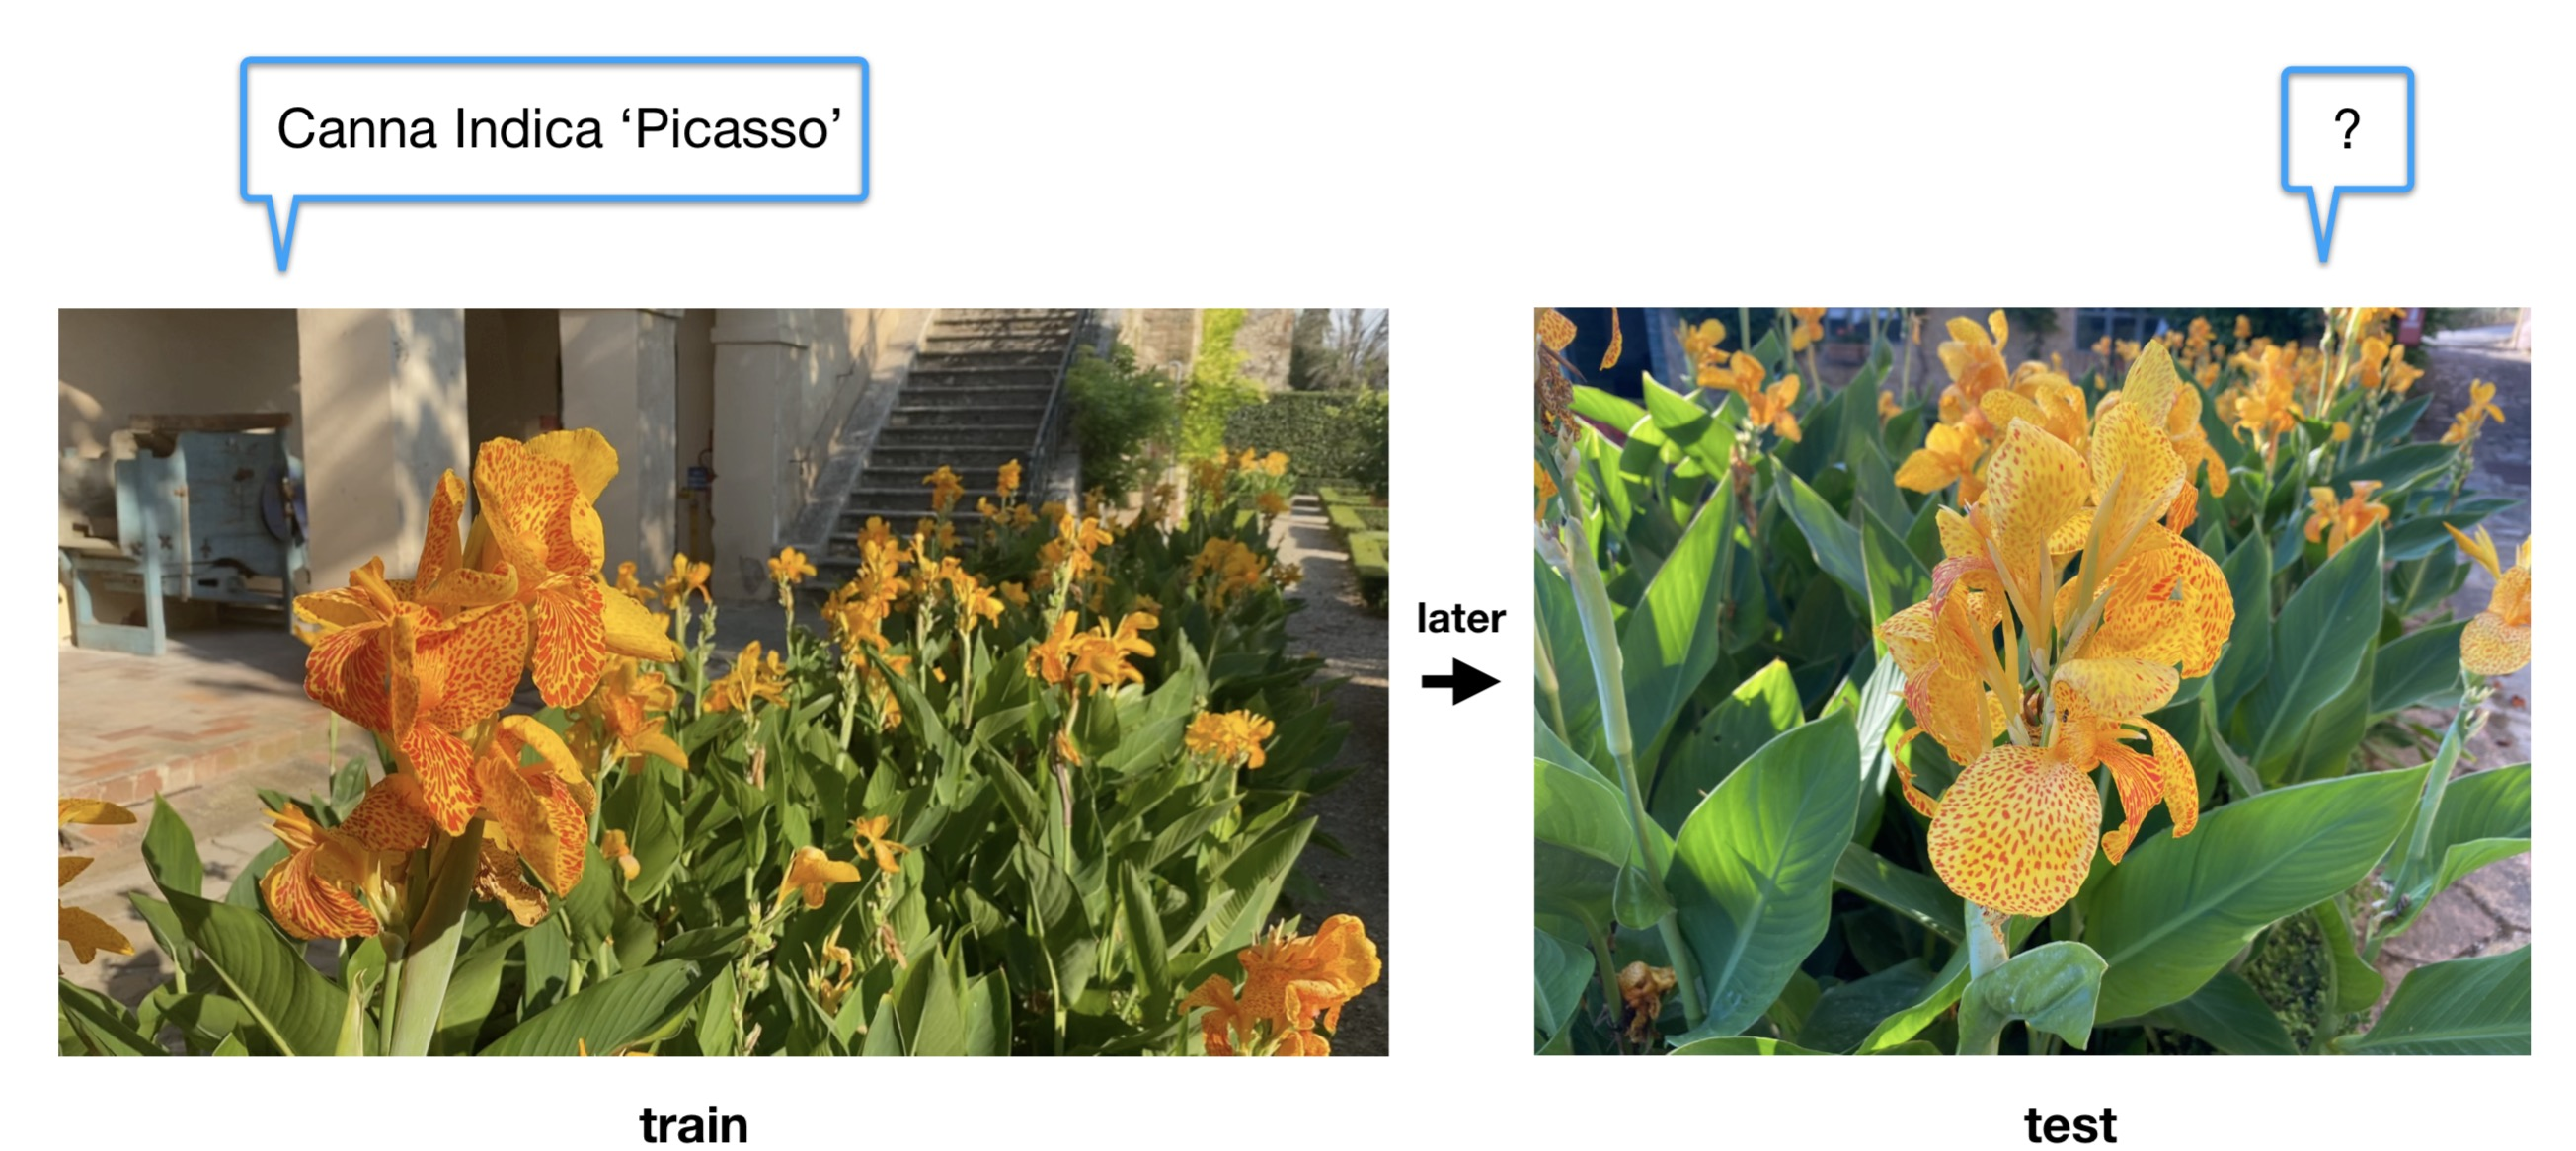
\includegraphics[height=6cm]{image/Jietu20220328-162621.jpg}

\end{frame}

%---------------------------------------------------------
\begin{frame}{Can a computer learn from a single example?}
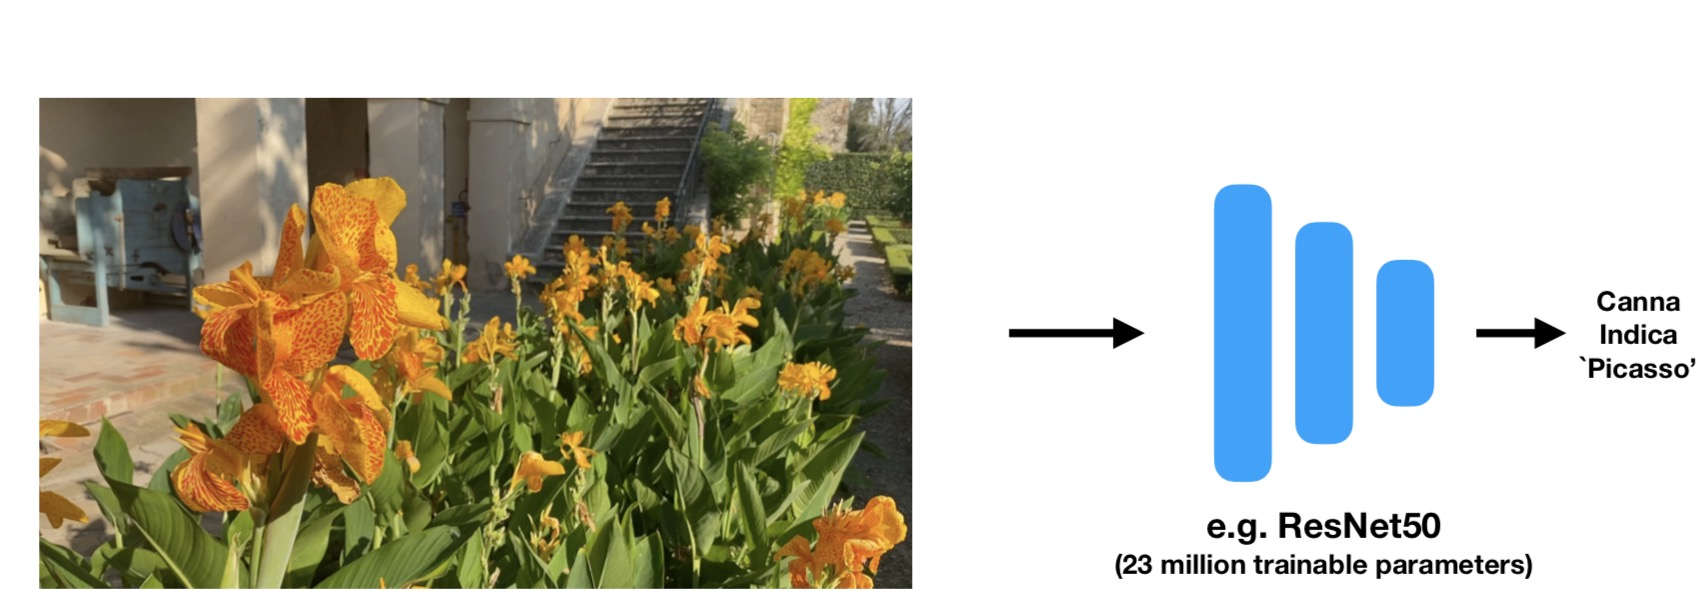
\includegraphics[height=5cm]{image/Jietu20220328-163023.jpg}

\hspace*{\fill} \
\hspace*{\fill} \
\pause
\centerline{\textbf{That won’t work :) Humans also don’t start from scratch.}}
\end{frame}


\begin{frame}{Transfer learning?}
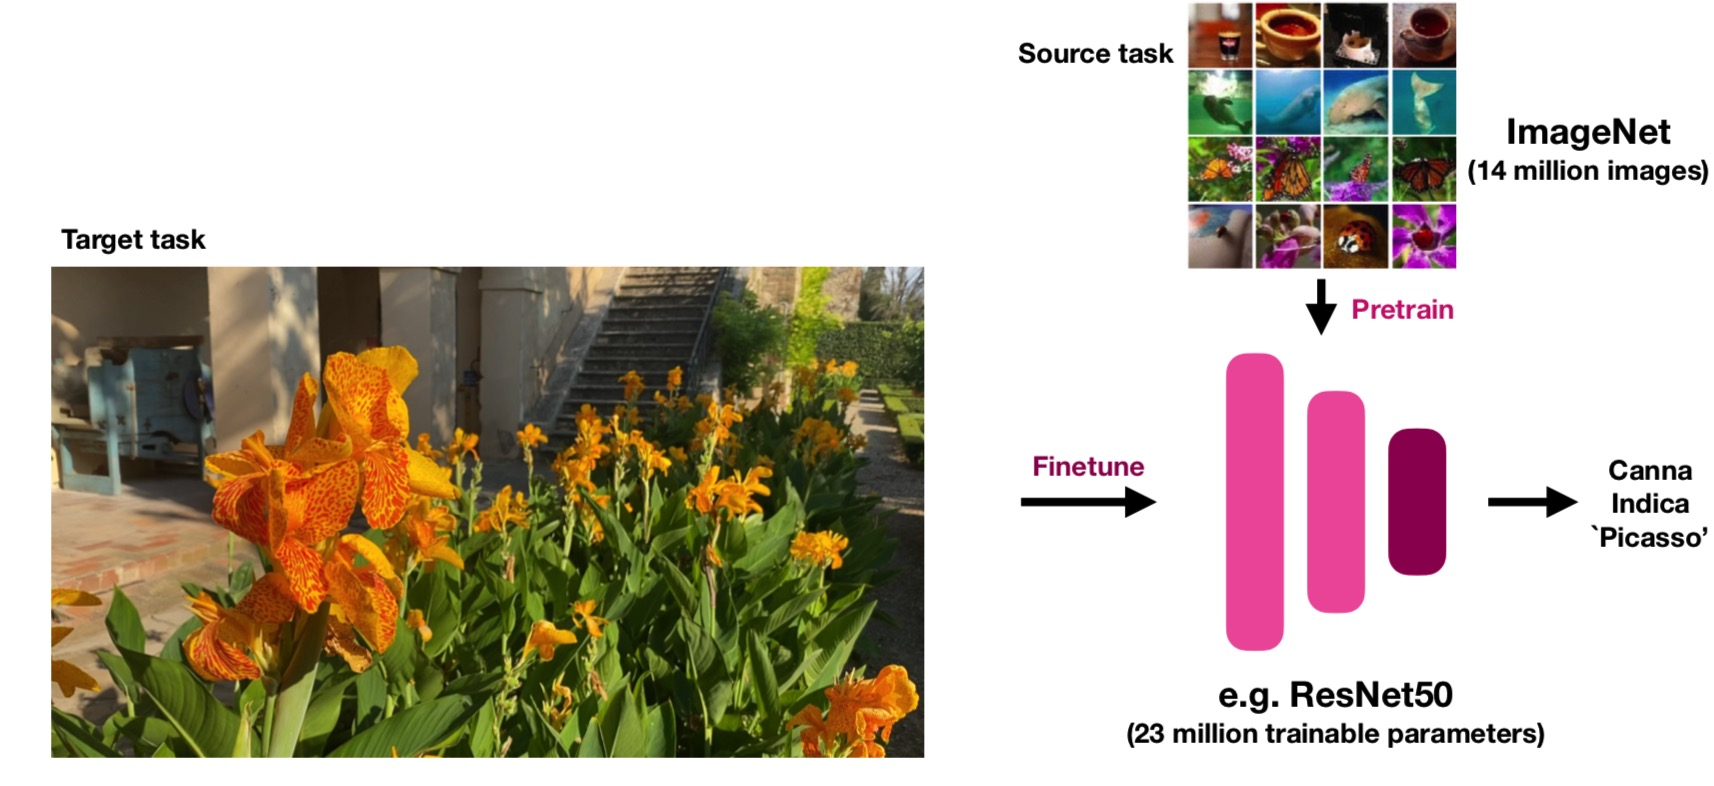
\includegraphics[height=6.5cm]{image/Jietu20220328-163705.jpg}

\pause
\small\centerline{\textbf{A single source task (e.g. ImageNet) may not generalize well to the test task.}}
\end{frame}

\begin{frame}{Meta-learning}{Learn over a series (or distribution) of many different tasks/episodes}
\centerline{\textit{\textcolor{red}{Inductive bias}: learn \textcolor{red}{assumptions} that you can to transfer to new tasks}}
\centerline{\textit{Prepare yourself to learn new things faster}}
\centering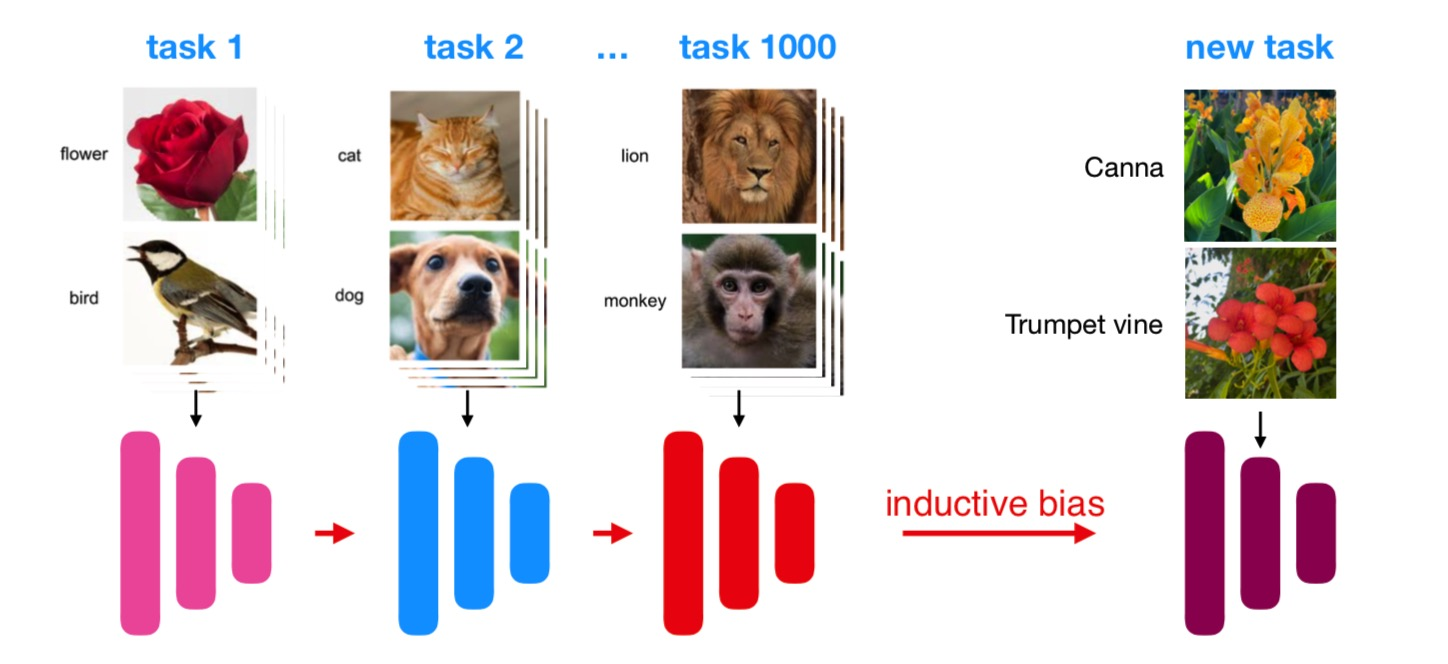
\includegraphics[height=5cm]{image/Jietu20220328-182859.jpg}

\pause
\leavevmode\hphantom{ }

\small\centerline{Useful in many real-life situations: rare events, test-time constraints, data collection costs, privacy issues,...}
\end{frame}

\begin{frame}{Inspired by human learning}
\centerline{We don’t transfer from a single source task, we learn across many, many tasks}
\centerline{We have a ‘drive’ to explore new, challenging, but doable, fun tasks}
 
\centering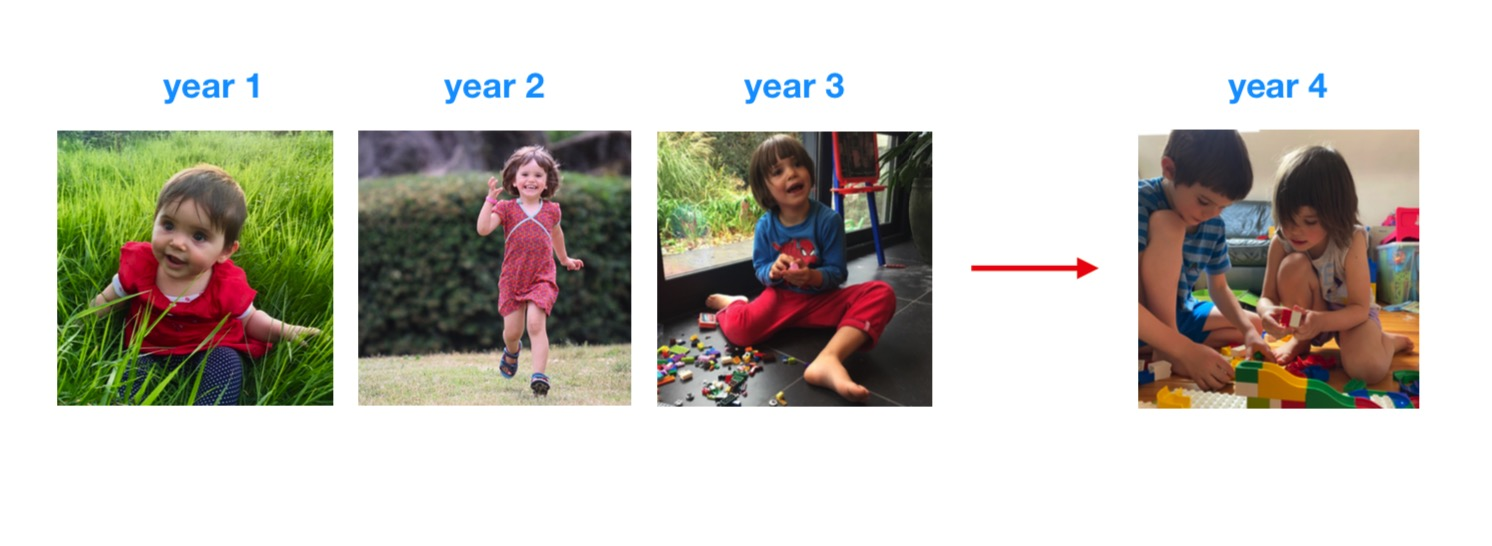
\includegraphics[height=5cm]{image/Jietu20220328-184210.jpg}

\end{frame}

\begin{frame}{Human-like Learning***}
\centerline{humans learn across tasks: less trial-and-error, less data, less compute}
\centerline{\textcolor{orange}{new tasks should be related to experience (doable, fun, interesting?)}}
 
\centering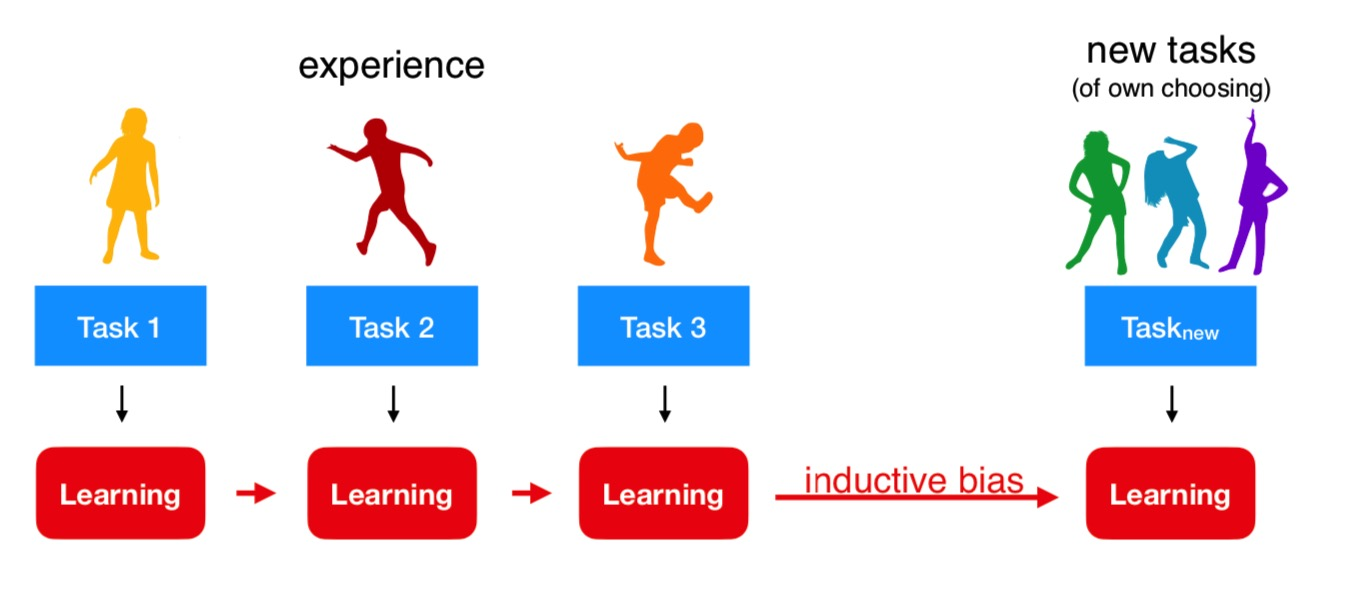
\includegraphics[height=5cm]{image/Jietu20220328-184546.jpg}

\centerline{\textit{key aspects of fast learning: compositionality, causality, \underline{learning to learn}}}
\end{frame}

\begin{frame}{Inductive bias (in language)}
\centerline{\textit{which assumptions do we make?}}
\centering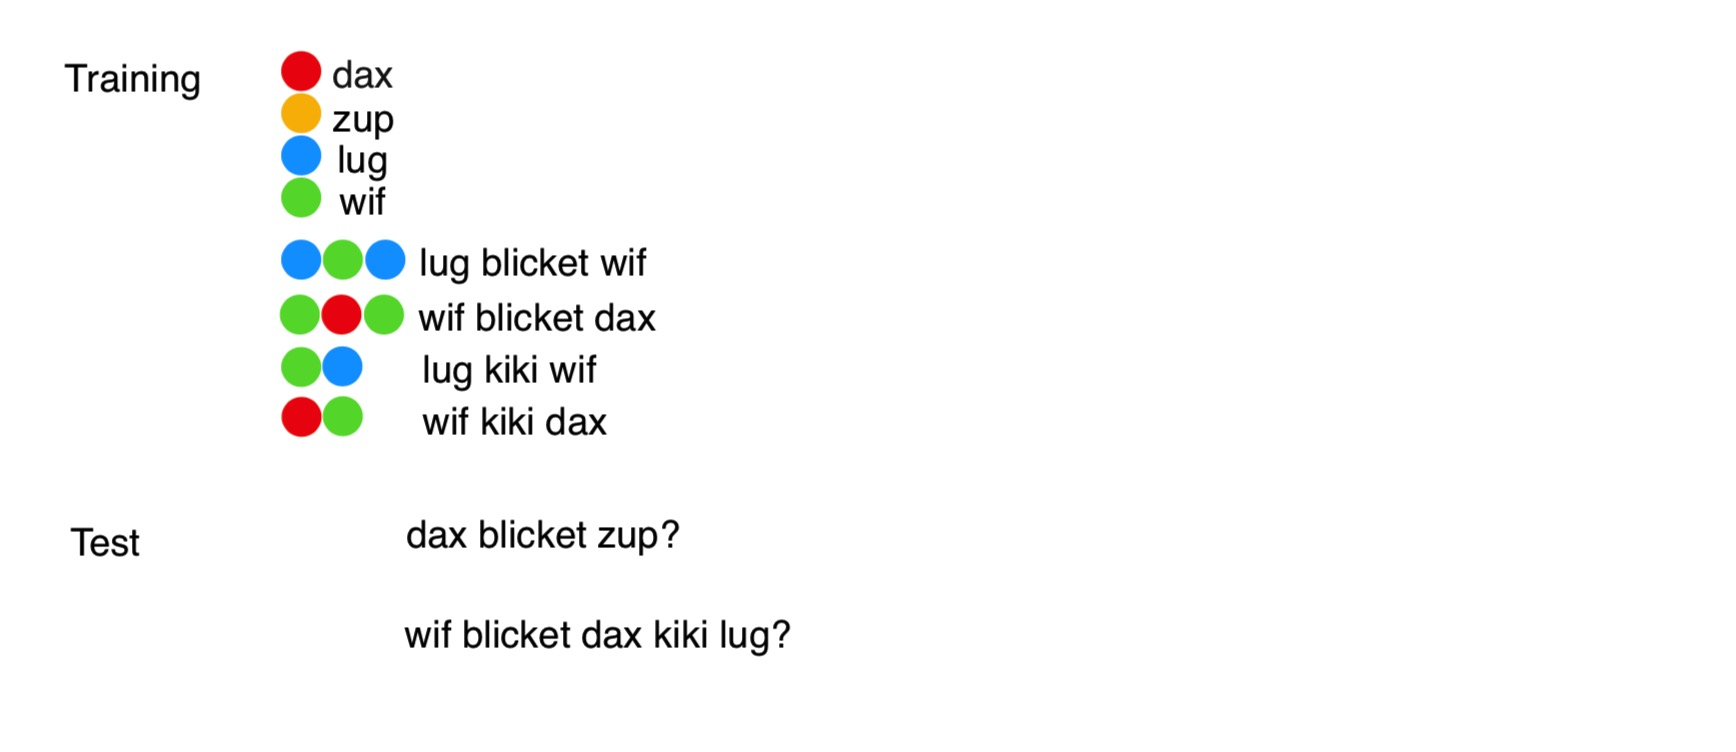
\includegraphics[height=6.2cm]{image/Jietu20220328-185829.jpg}

\end{frame}

\begin{frame}{Inductive bias (in language)}
\centerline{\textit{which assumptions do we make?}}
\centering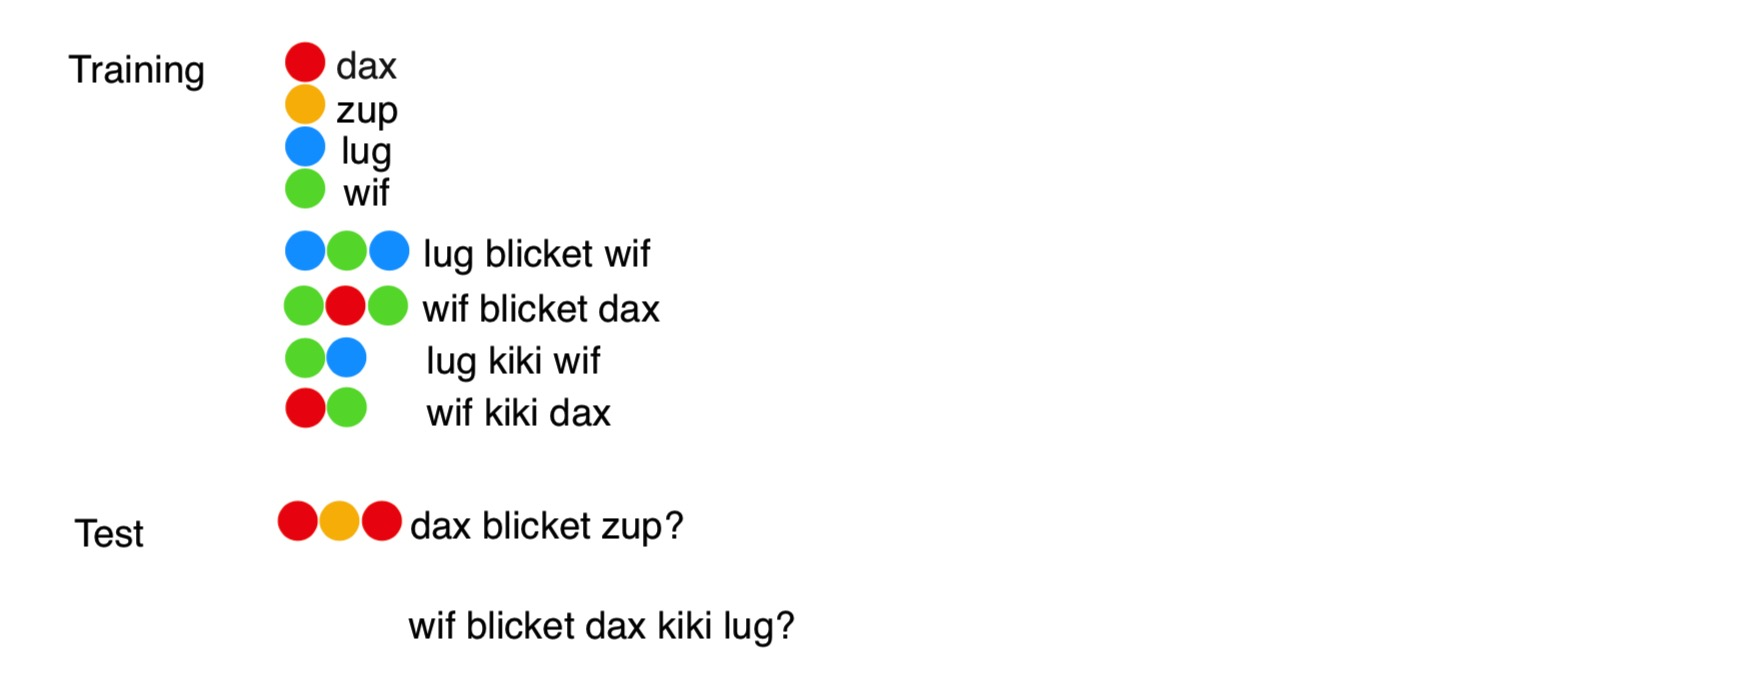
\includegraphics[height=6cm]{image/Jietu20220328-185953.jpg}

\end{frame}

\begin{frame}{Inductive bias (in language)}
\centerline{\textit{which assumptions do we make?}}
\centering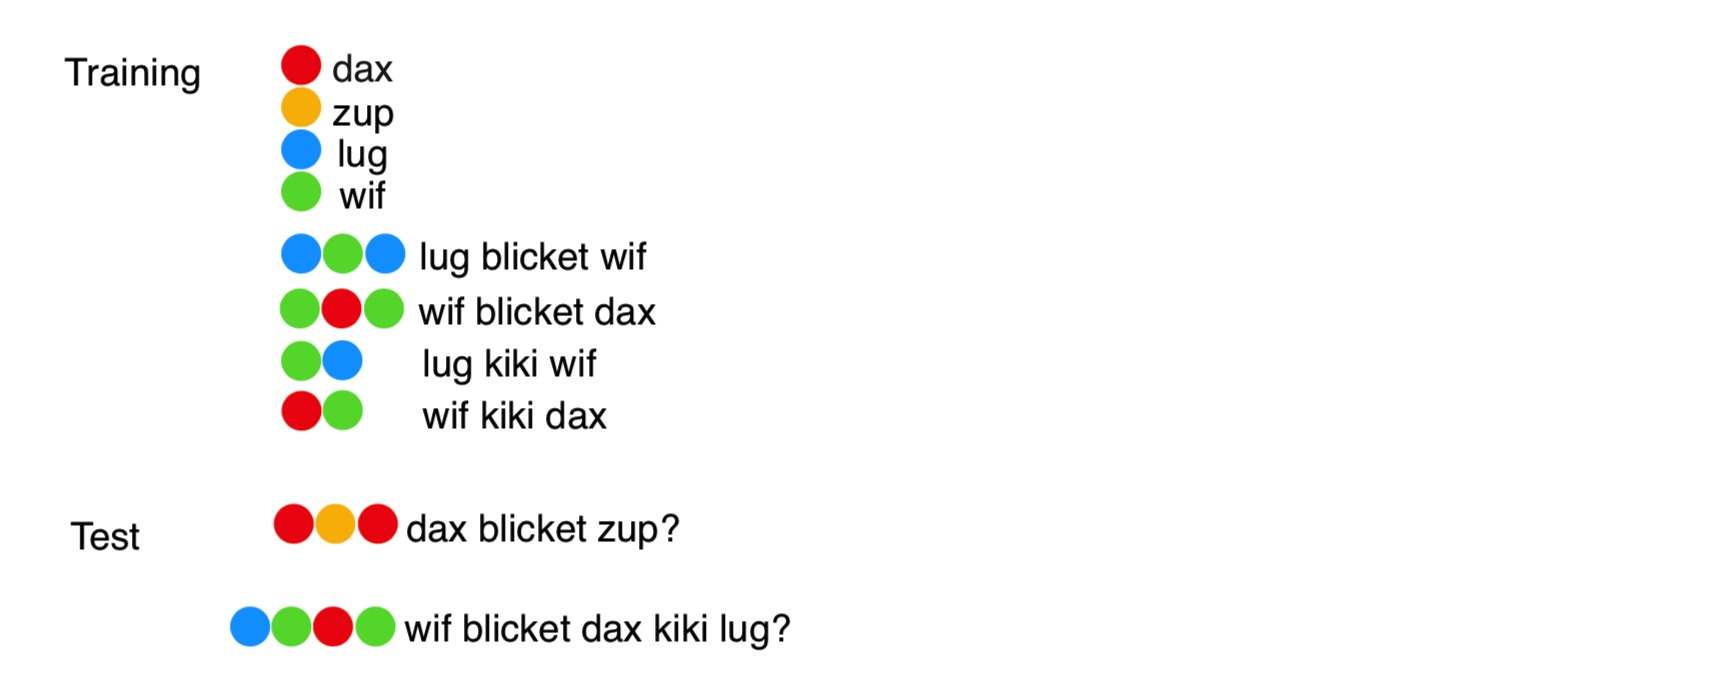
\includegraphics[height=5.9cm]{image/Jietu20220328-190213.jpg}

\end{frame}

\begin{frame}{Inductive bias (in language)}
\centerline{\textit{which assumptions do we make?}}
\centering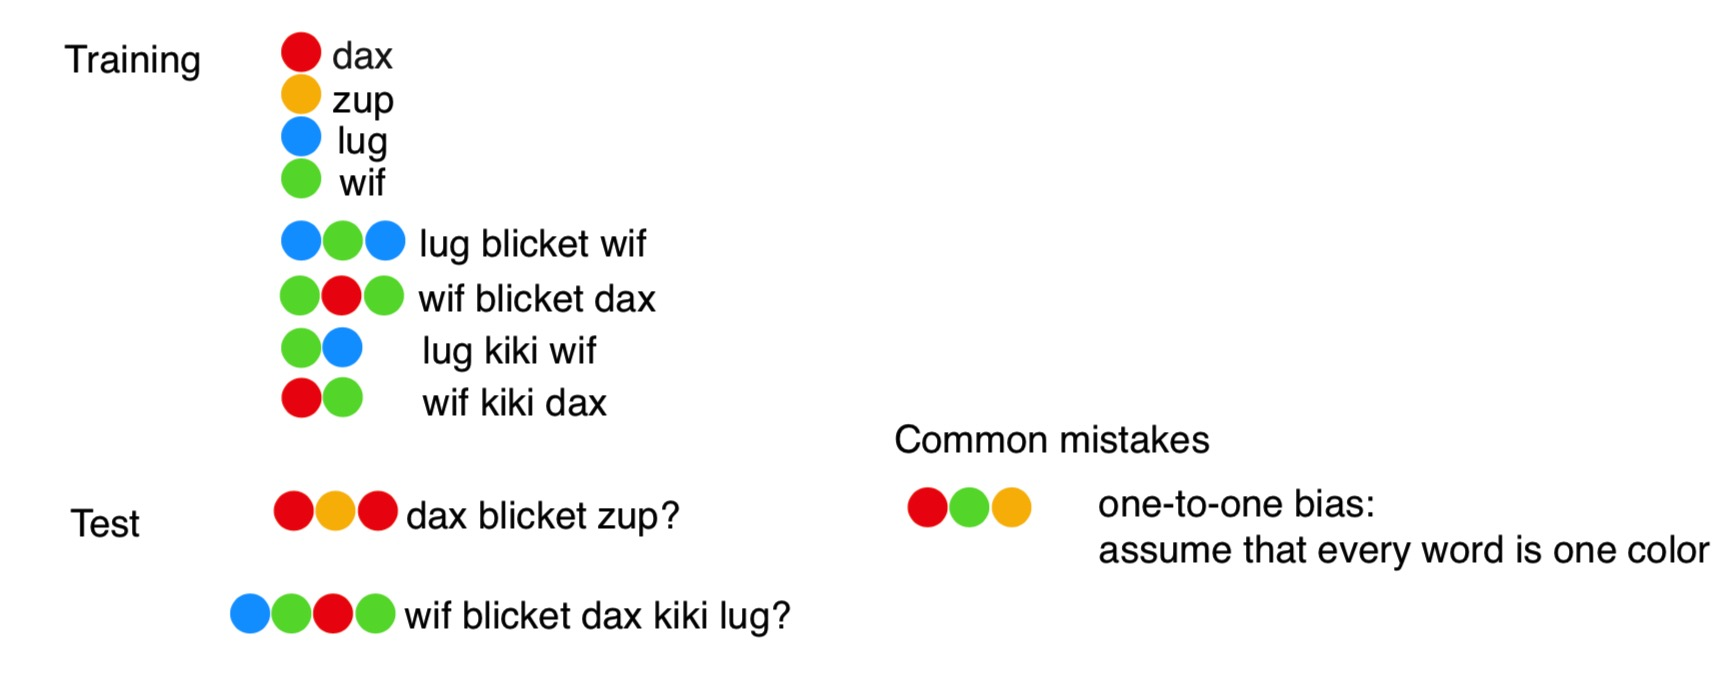
\includegraphics[height=5.9cm]{image/Jietu20220328-190532.jpg}

\end{frame}

\begin{frame}{Inductive bias (in language)}
\centerline{\textit{which assumptions do we make?}}
\centering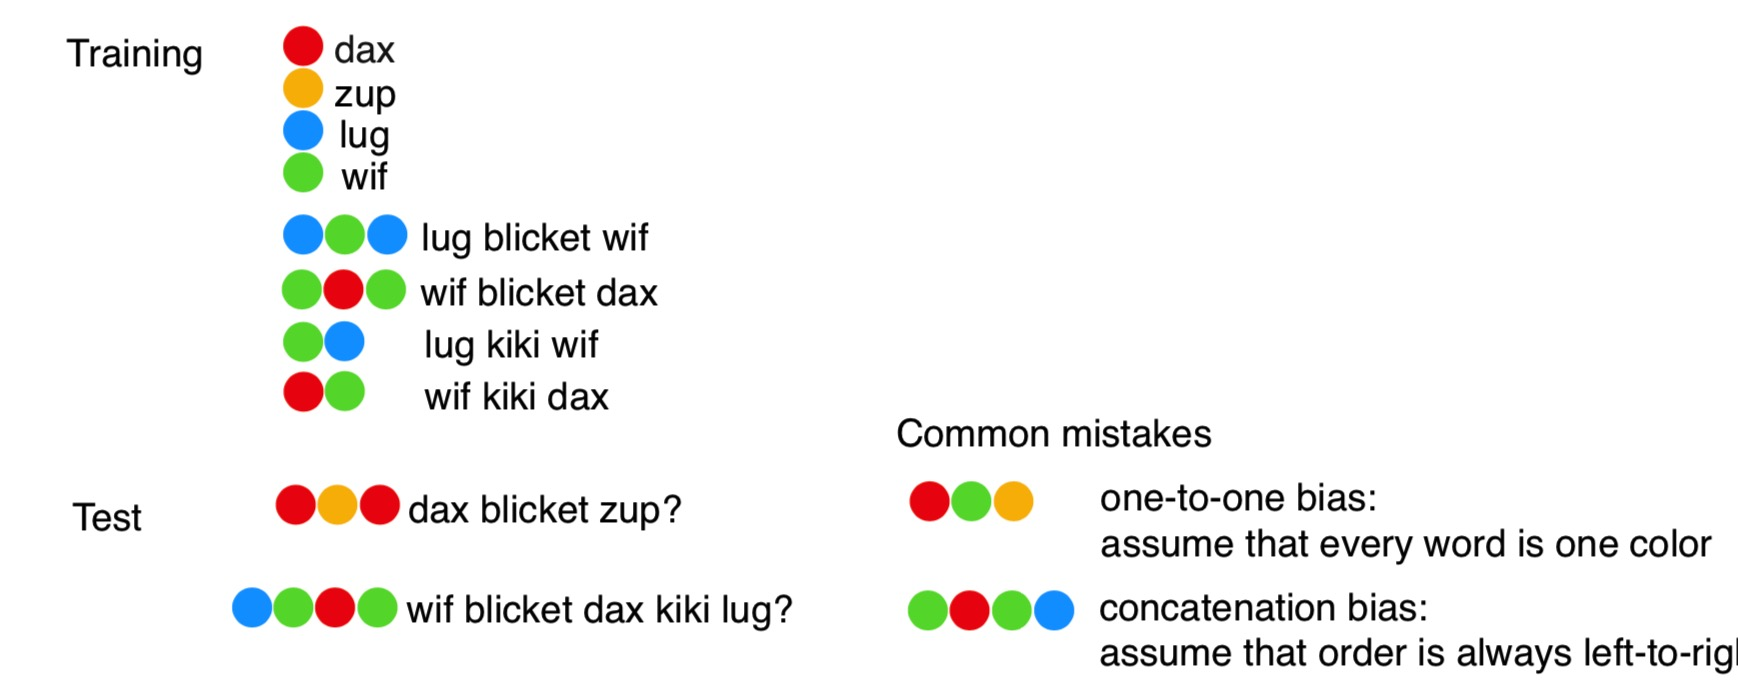
\includegraphics[height=5.9cm]{image/Jietu20220328-190839.jpg}

\end{frame}

\begin{frame}{What if there is no training data?}
\centerline{\textit{we can still solve problems by making assumptions}}
\centering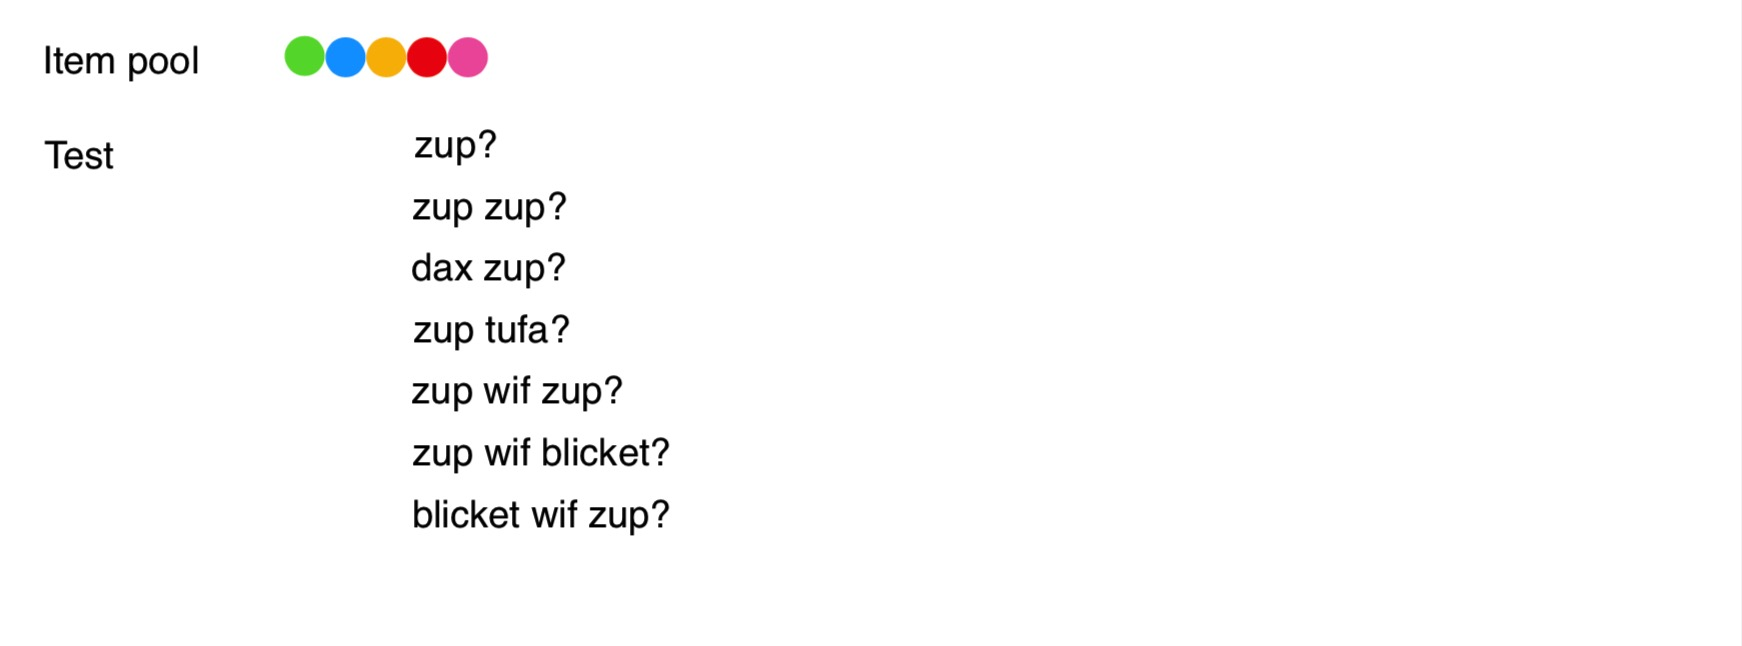
\includegraphics[height=5.5cm]{image/Jietu20220328-191412.jpg}

\end{frame}

\begin{frame}{What if there is no training data?}
\centerline{\textit{we can still solve problems by making assumptions}}
\centering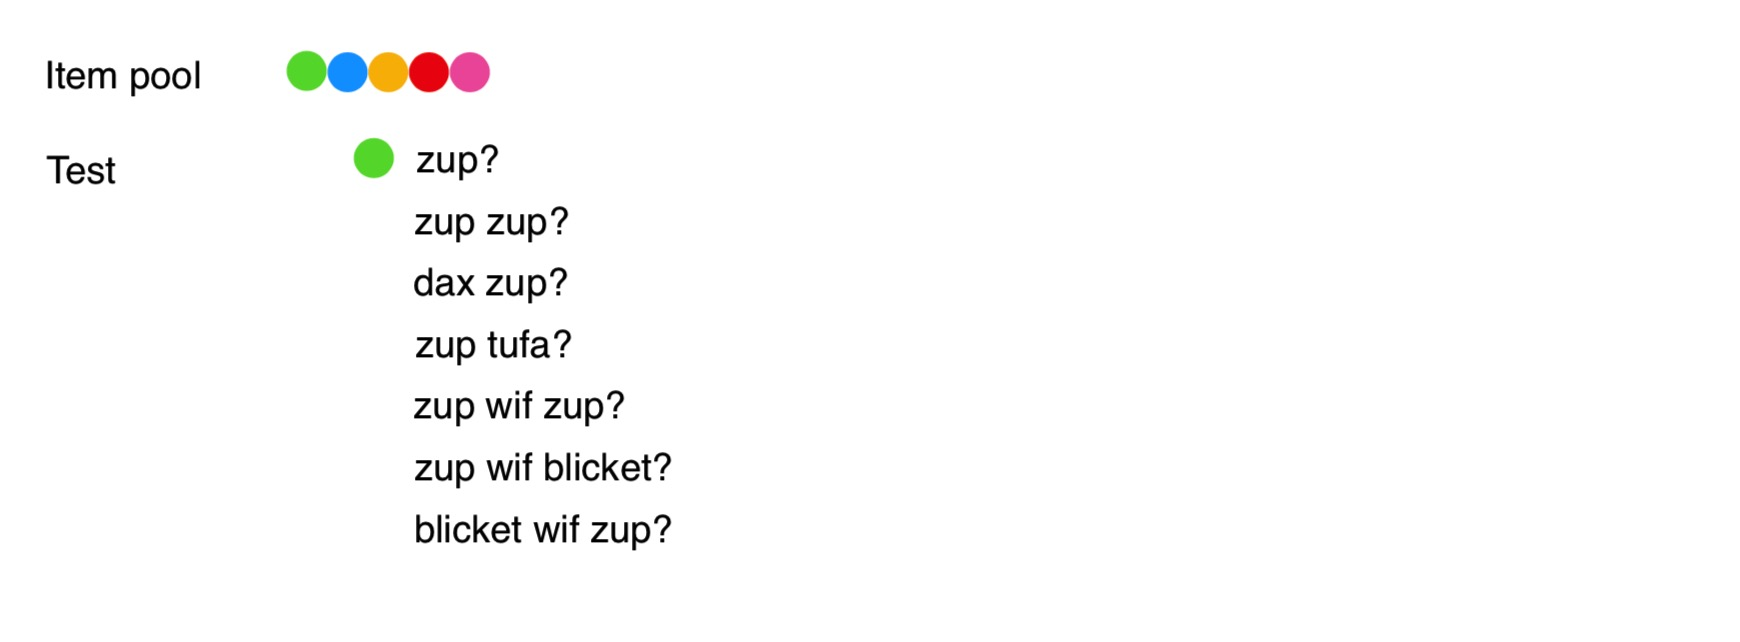
\includegraphics[height=5.5cm]{image/Jietu20220328-191823.jpg}

\end{frame}

\begin{frame}{What if there is no training data?}
\centerline{\textit{we can still solve problems by making assumptions}}
\centering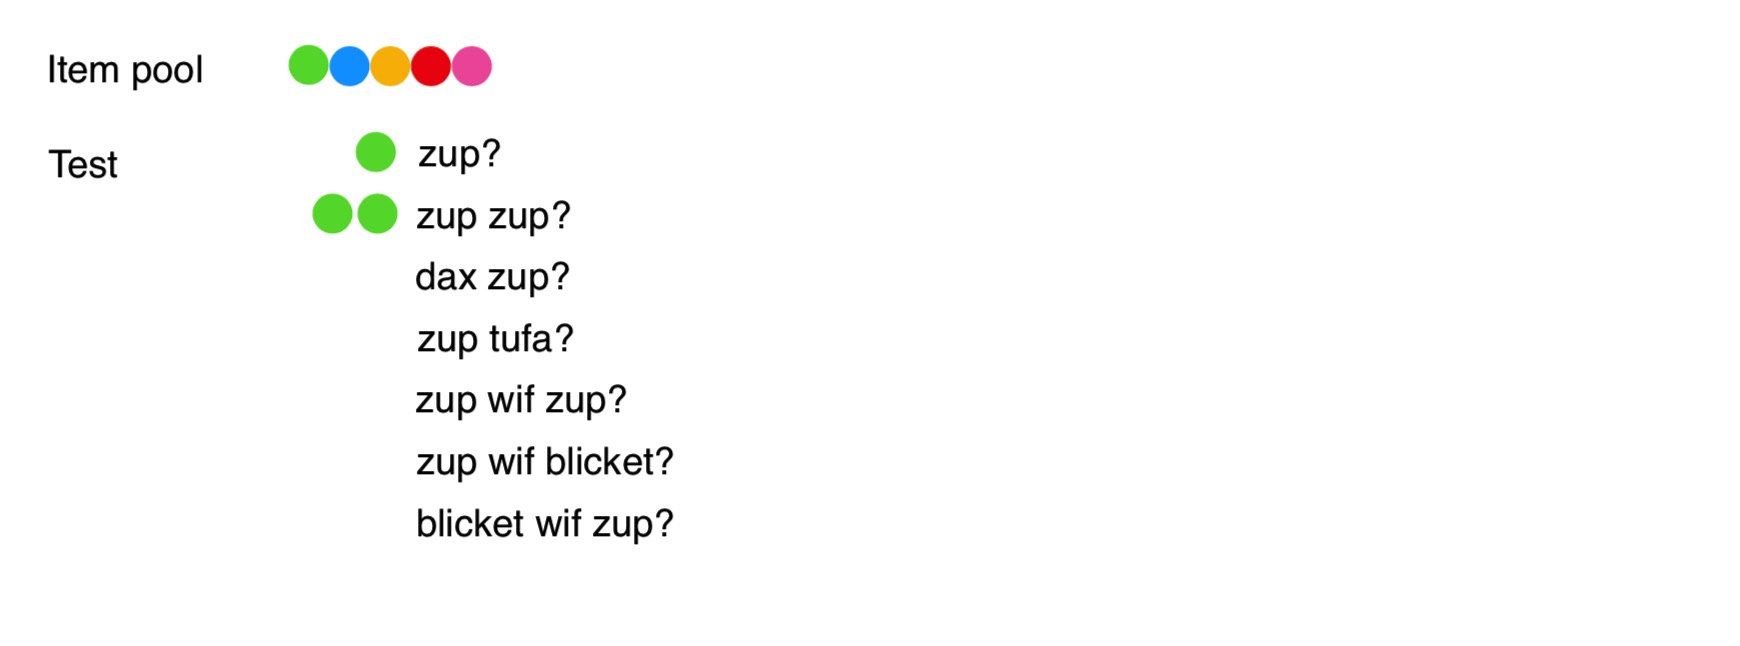
\includegraphics[height=5.5cm]{image/Jietu20220328-191448.jpg}

\end{frame}

\begin{frame}{What if there is no training data?}
\centerline{\textit{we can still solve problems by making assumptions}}
\centering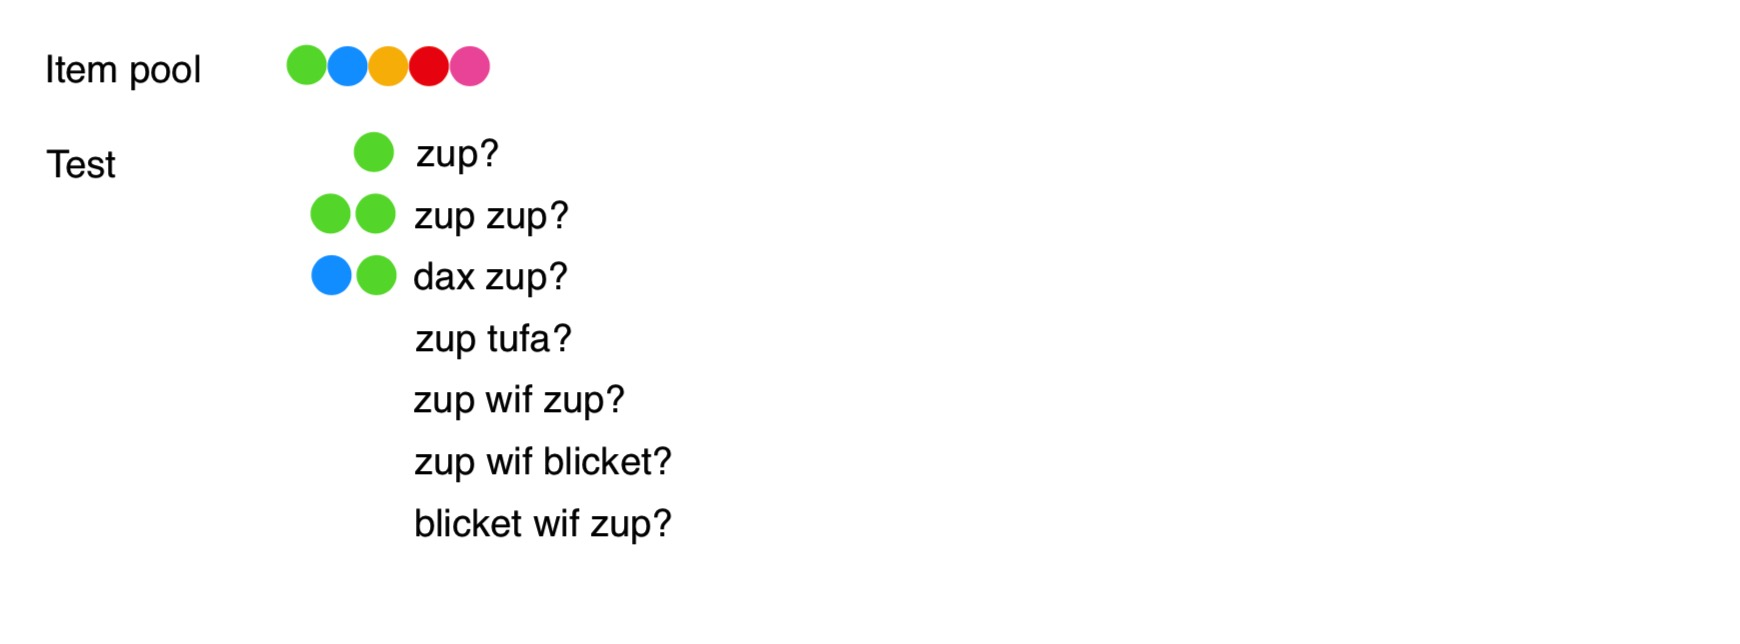
\includegraphics[height=5.5cm]{image/Jietu20220328-191531.jpg}

\end{frame}

\begin{frame}{What if there is no training data?}
\centerline{\textit{we can still solve problems by making assumptions}}
\centering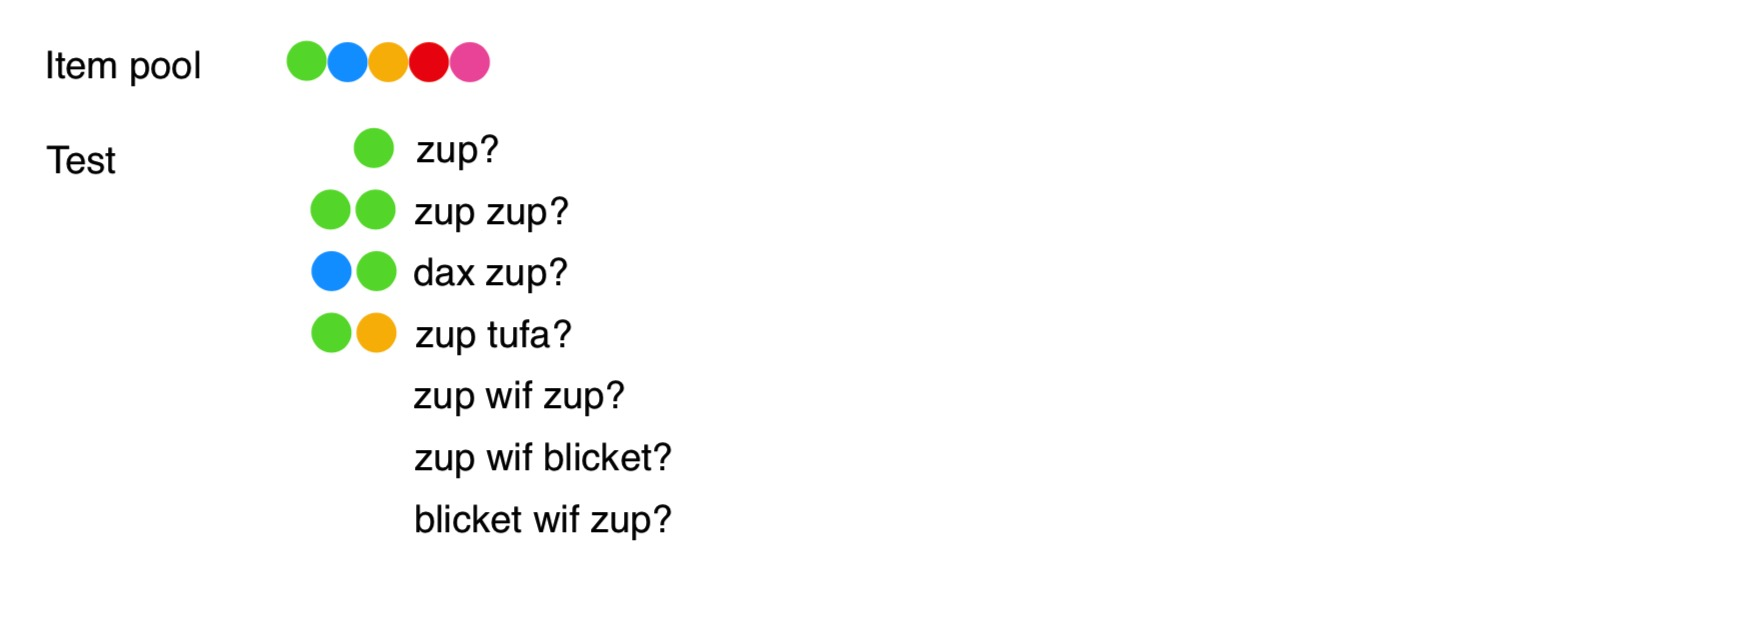
\includegraphics[height=5.5cm]{image/Jietu20220328-192202.jpg}

\end{frame}

\begin{frame}{What if there is no training data?}
\centerline{\textit{we can still solve problems by making assumptions}}
\centering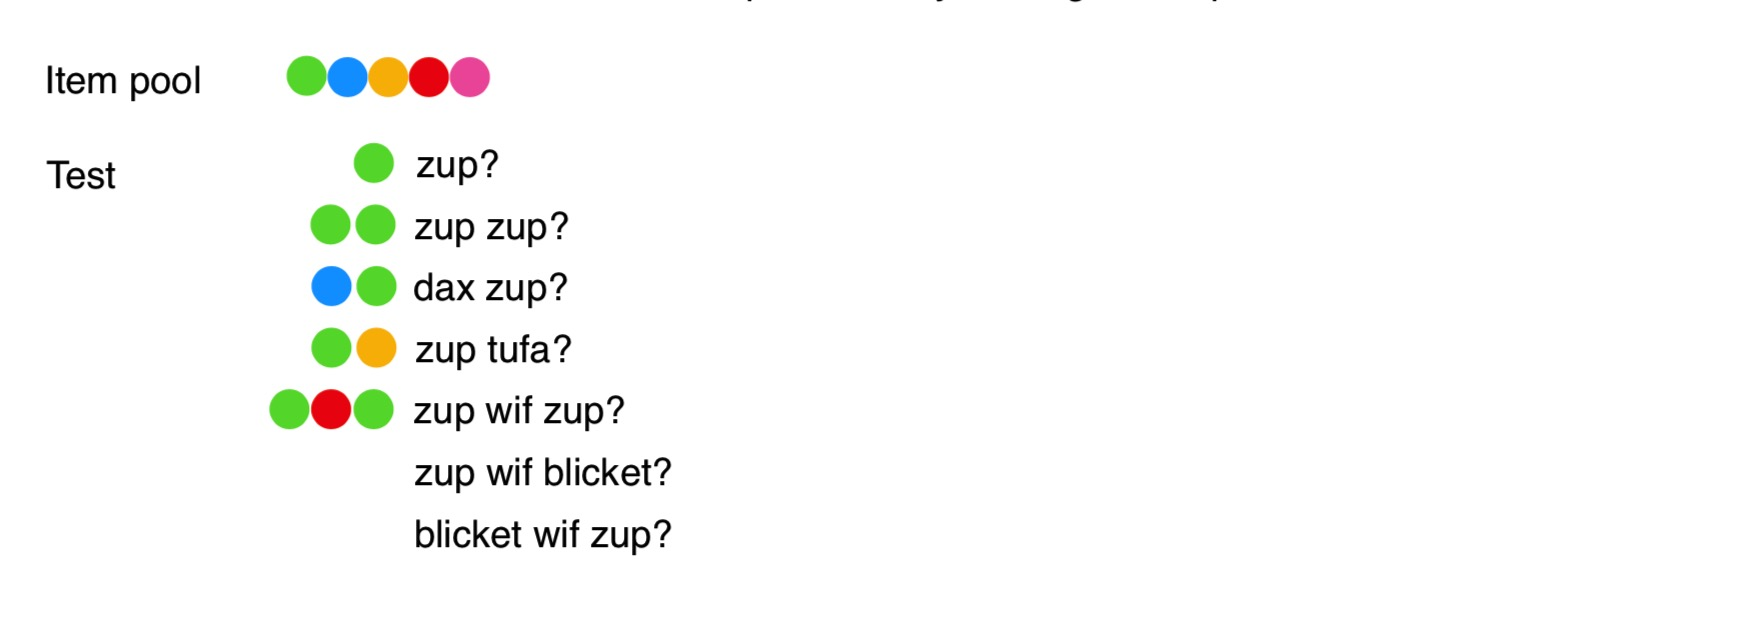
\includegraphics[height=5.5cm]{image/Jietu20220328-192229.jpg}

\end{frame}
\begin{frame}{What if there is no training data?}
\centerline{\textit{we can still solve problems by making assumptions}}
\centering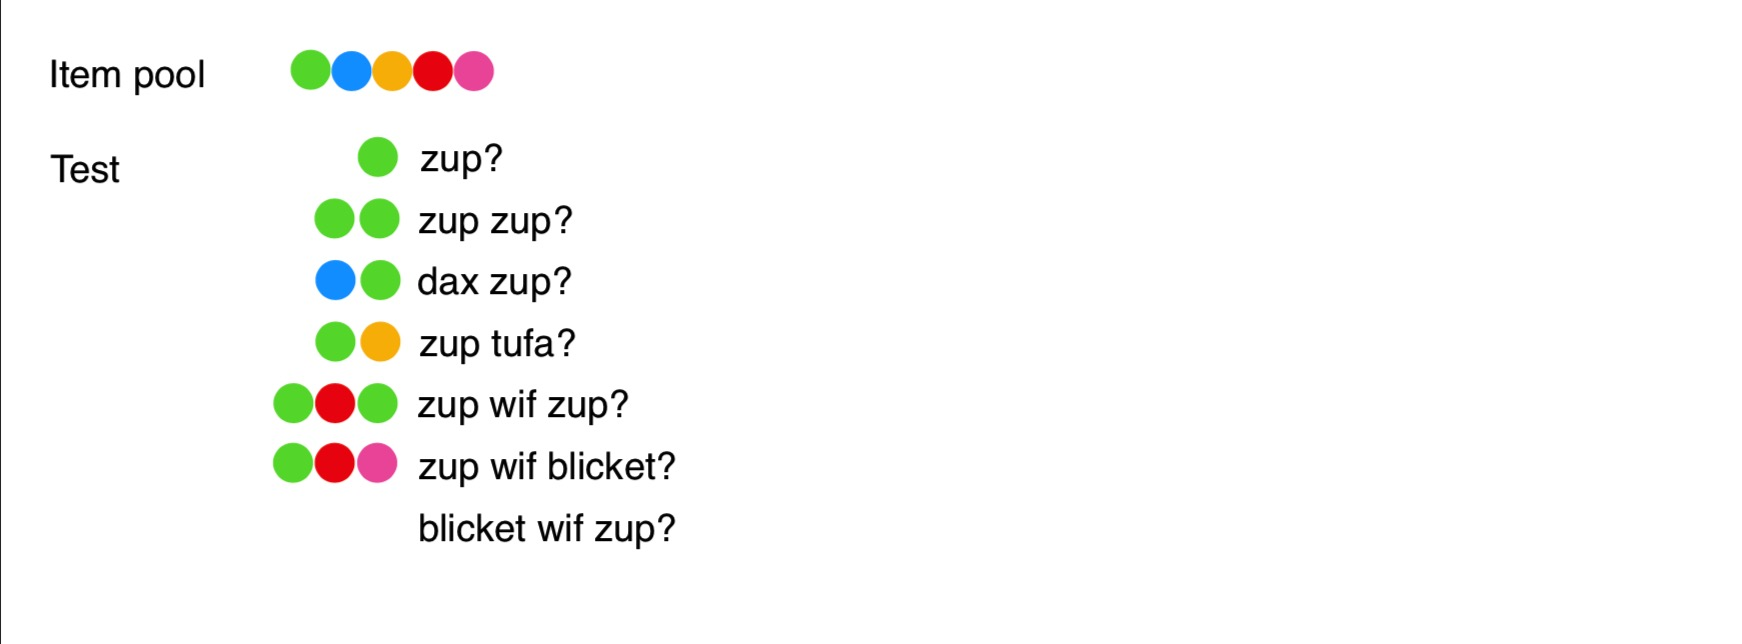
\includegraphics[height=5.5cm]{image/Jietu20220328-192318.jpg}

\end{frame}
\begin{frame}{What if there is no training data?}
\centerline{\textit{we can still solve problems by making assumptions}}
\centering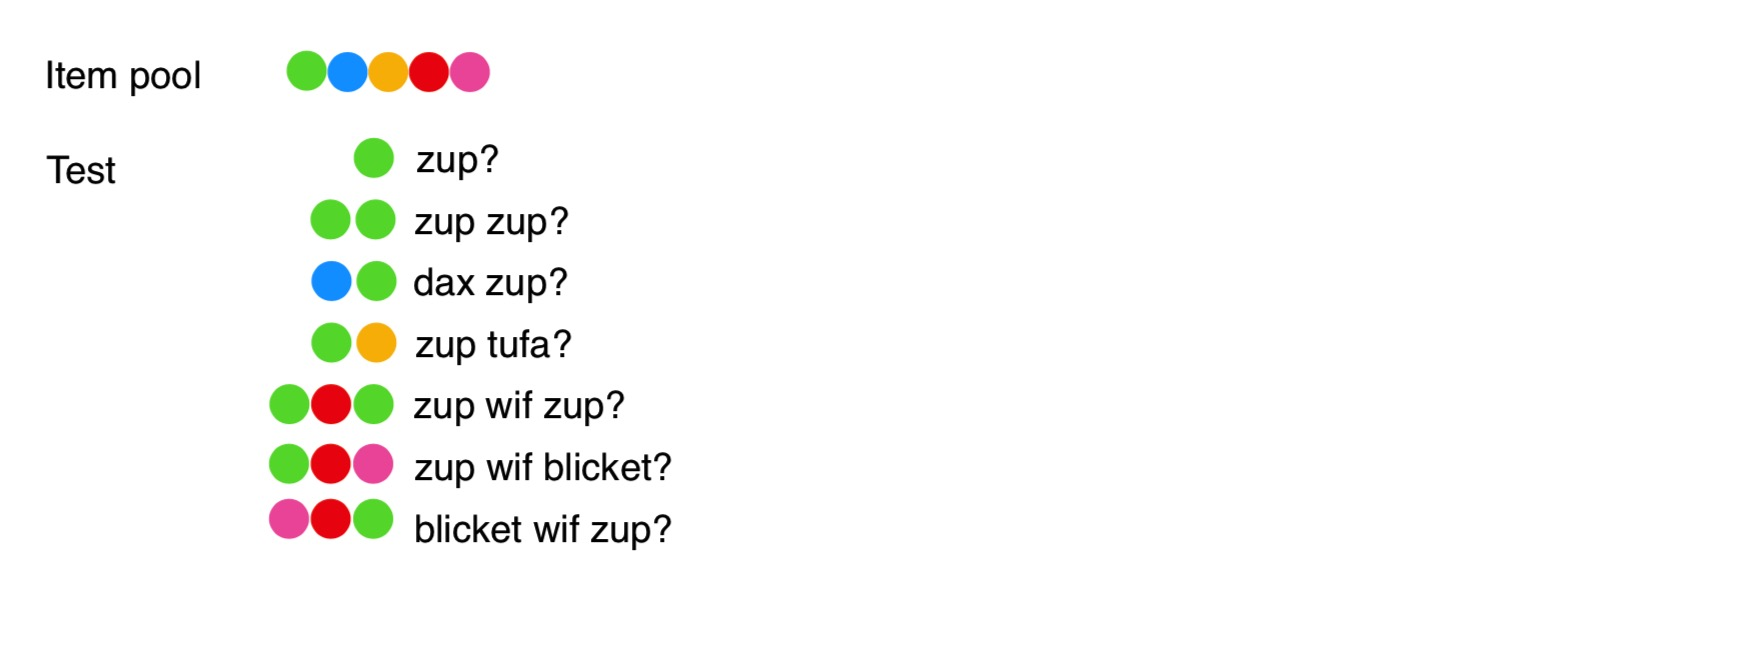
\includegraphics[height=5.5cm]{image/Jietu20220328-192345.jpg}

\end{frame}
\begin{frame}{What if there is no training data?}
\centerline{\textit{we can still solve problems by making assumptions}}
\centering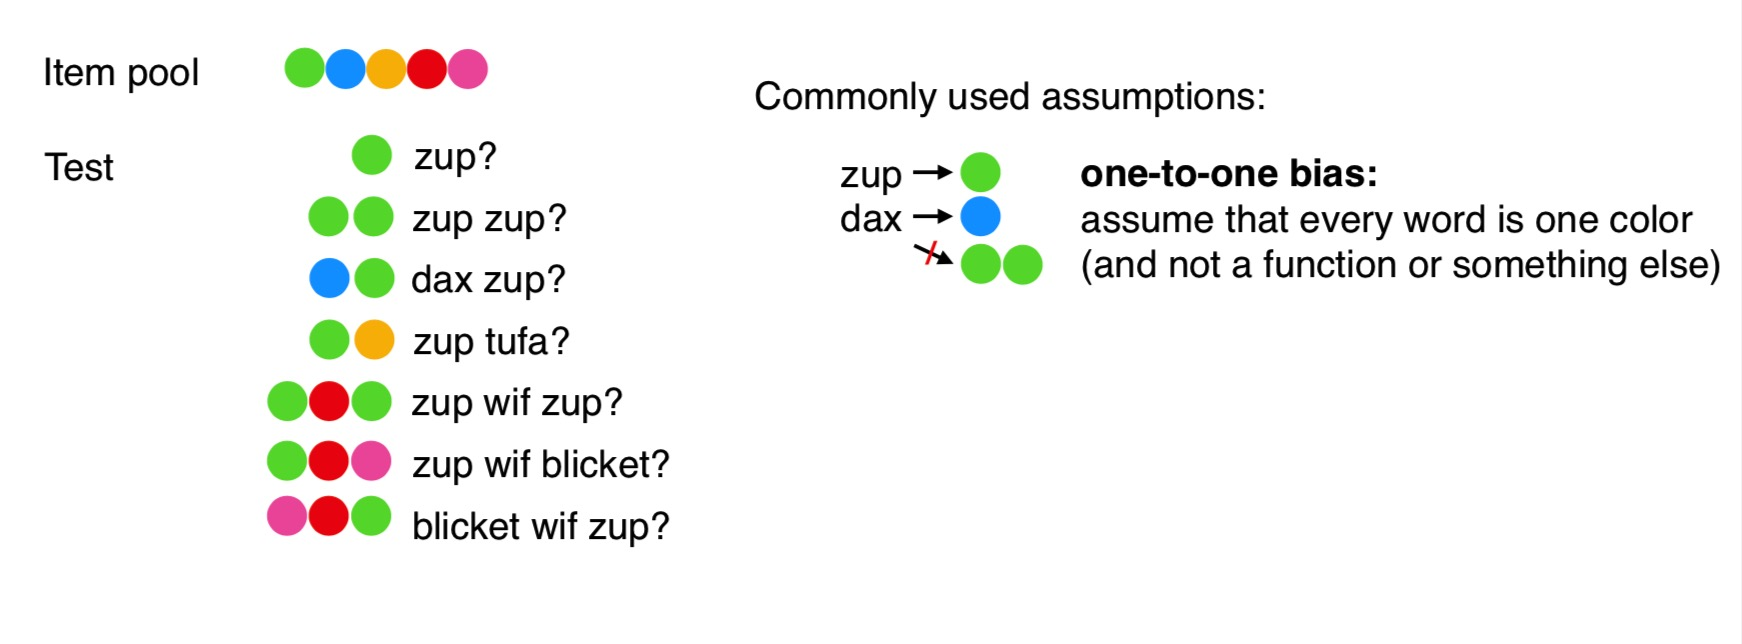
\includegraphics[height=5.5cm]{image/Jietu20220328-192403.jpg}

\end{frame}
\begin{frame}{What if there is no training data?}
\centerline{\textit{we can still solve problems by making assumptions}}
\centering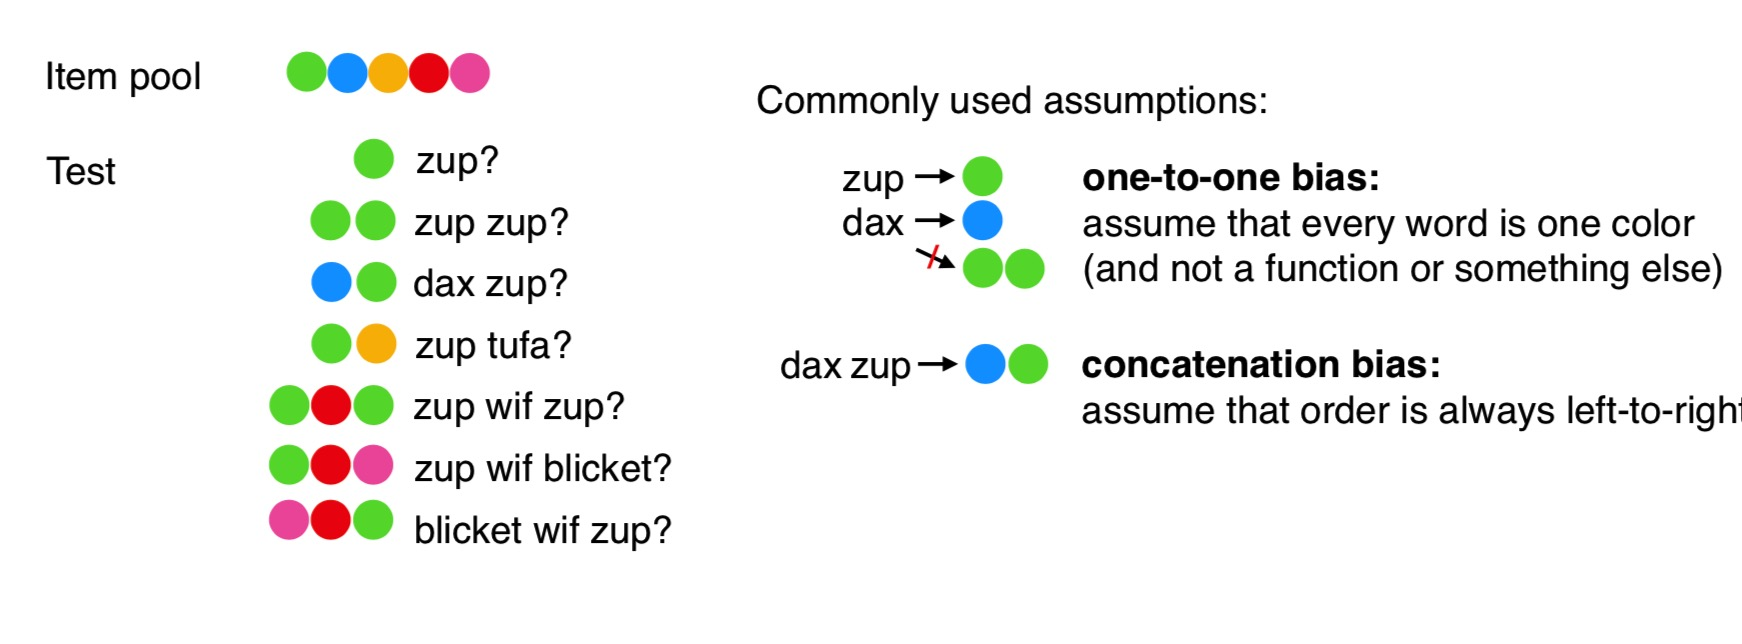
\includegraphics[height=5.5cm]{image/Jietu20220328-192435.jpg}

\end{frame}
\begin{frame}{What if there is no training data?}
\centerline{\textit{we can still solve problems by making assumptions}}
\centering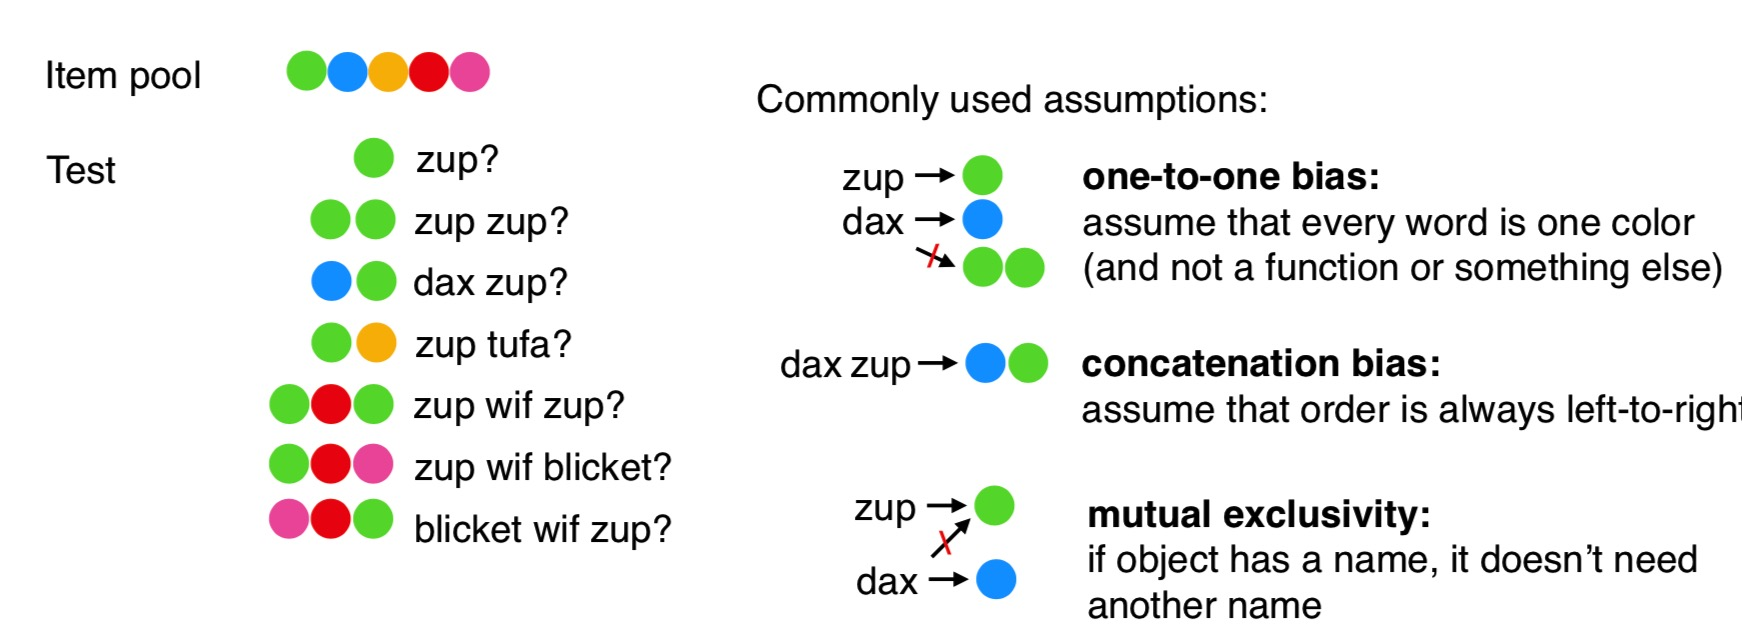
\includegraphics[height=5.5cm]{image/Jietu20220328-192503.jpg}
\pause
\leavevmode\hphantom{ }

\small\centerline{Humans \textit{assume} that words have consistent meanings and follow input/output constraints}
\pause
\small\centerline{\textbf{These assumptions \textcolor{red}{(inductive biases)} are necessary for learning quickly}}
\end{frame}

\begin{frame}{Meta-learning inductive biases}
\centerline{\textit{Capture \textcolor{red}{useful assumptions} from the data - that can often not be easily expressed}}
\centering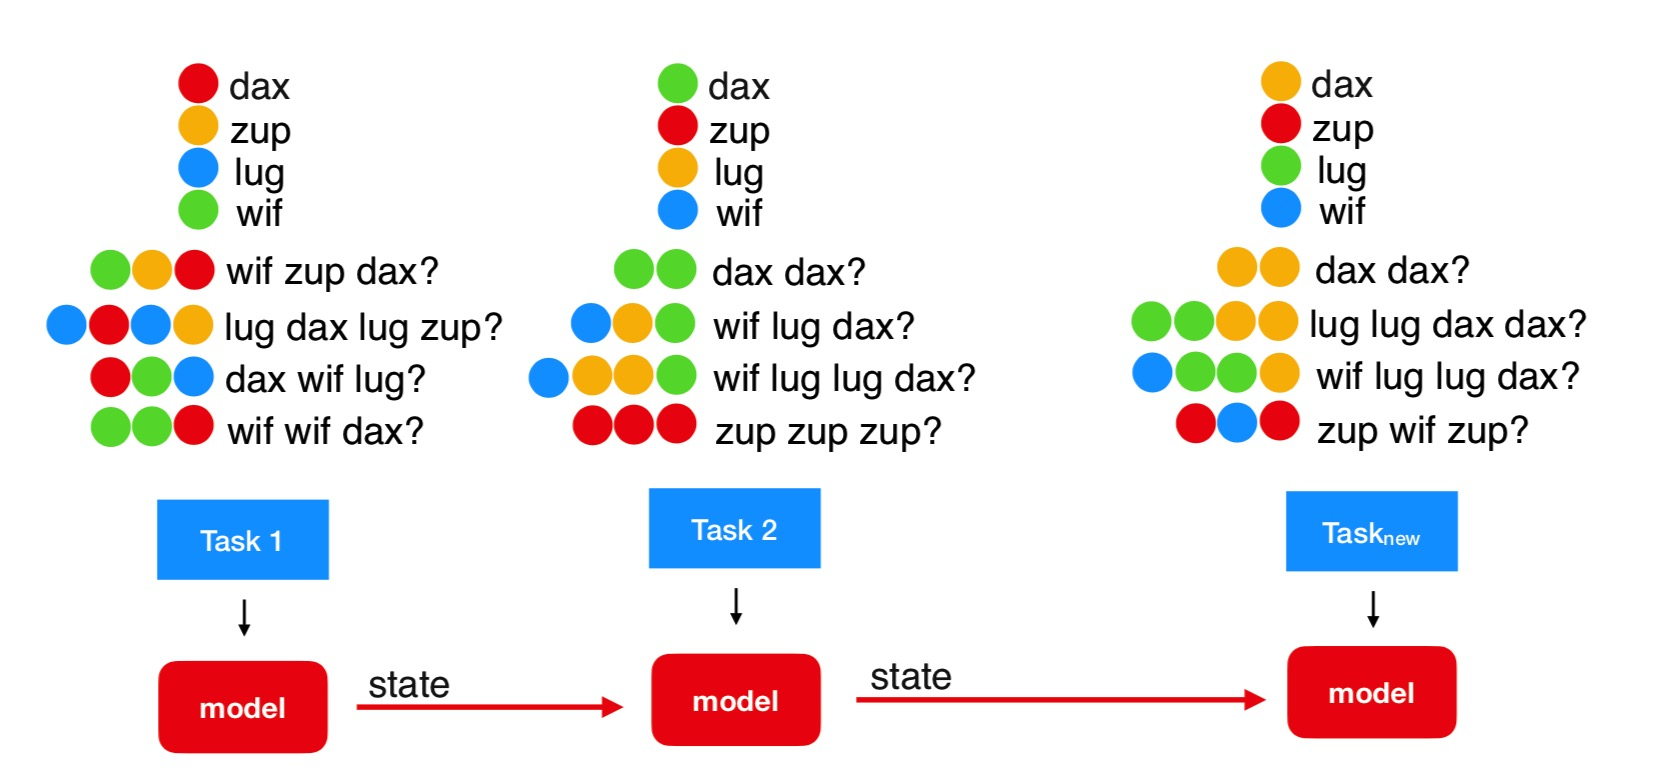
\includegraphics[height=6cm]{image/Jietu20220328-193434.jpg}

\end{frame}

\begin{frame}{Meta-learning goal}
\centerline{learn \textit{minimal} inductive biases from prior tasks instead of constructing manual ones }
\centerline{should still generalize well (otherwise you meta-overfit)}
\centering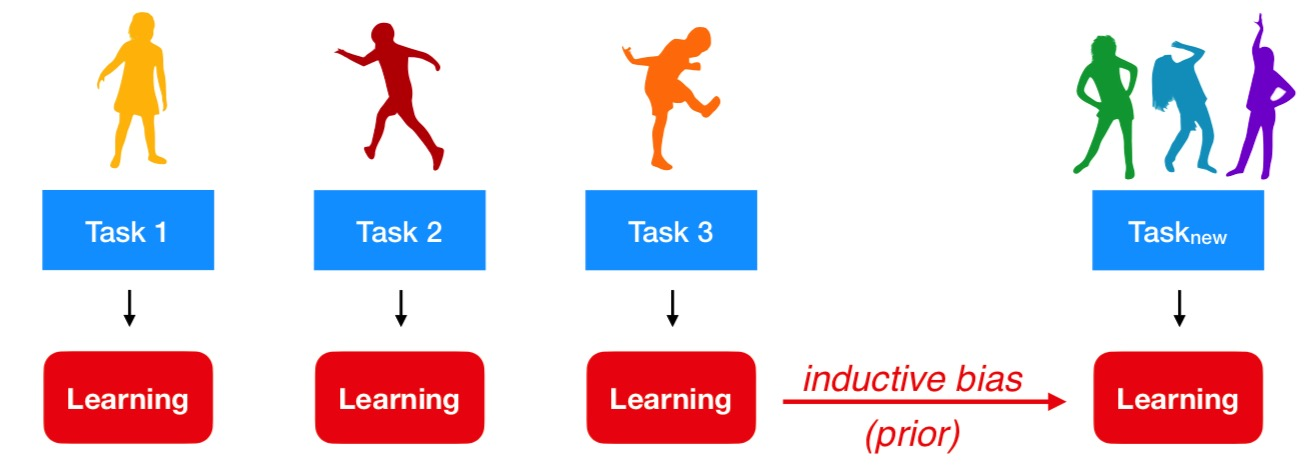
\includegraphics[height=3.5cm]{image/Jietu20220328-193722.jpg}


\textbf{Inductive bias:} any assumptions added to training data to learn more effectively. E.g:
\begin{itemize}
  \item Instead of \textcolor{red}{general model architectures}, \textcolor{green}{learn better architectures (and hyperparameters)}
  \item Instead of \textcolor{red}{starting from random weights}, \textcolor{green}{learn good initial weights}
  \item Instead of \textcolor{red}{standard loss/reward function}, \textcolor{green}{learn a better loss/reward function}
\end{itemize}
\end{frame}

\begin{frame}{What can we learn to learn?}
\centerline{\textit{3 pillars}}
\centering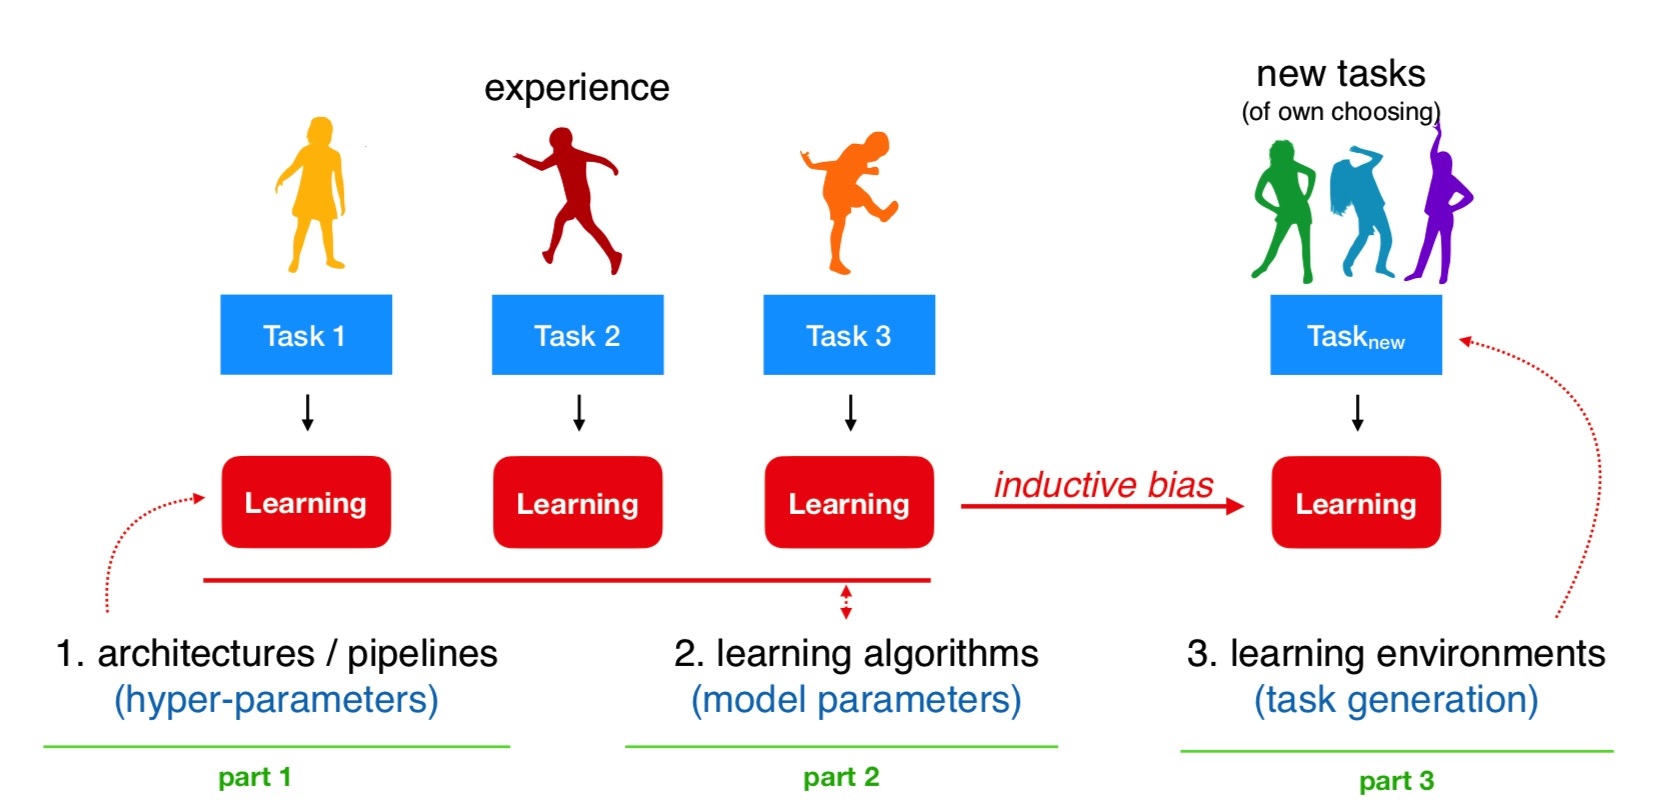
\includegraphics[height=5.5cm]{image/Jietu20220328-194451.jpg}

\end{frame}
\begin{frame}{What can we learn to learn?}
\centerline{\textit{3 pillars}}
\centering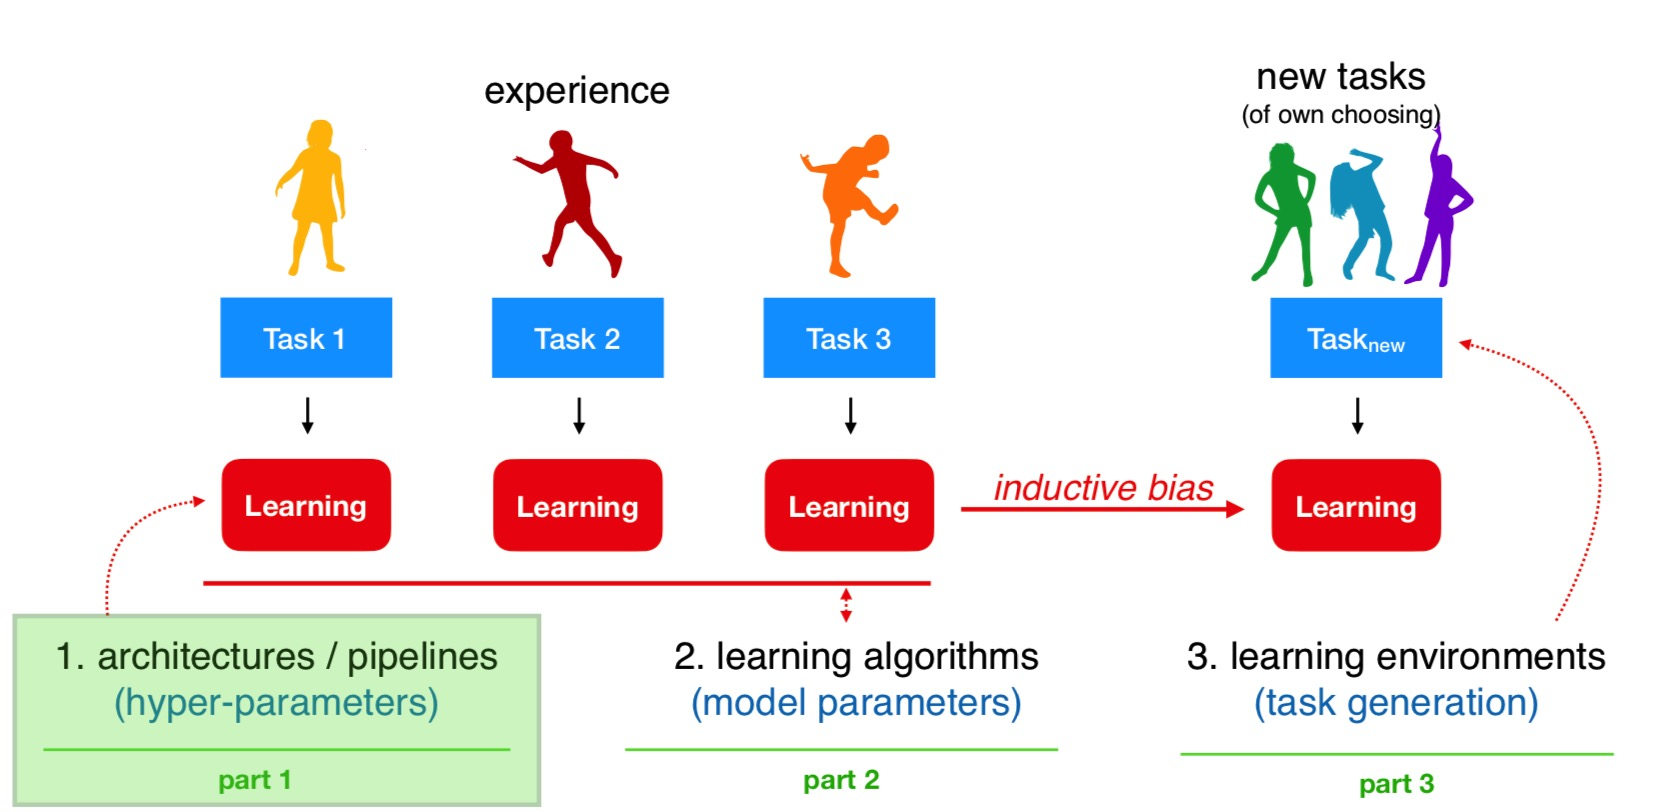
\includegraphics[height=5.5cm]{image/Jietu20220328-194520.jpg}

\end{frame}
\begin{frame}{Terminology}

\centering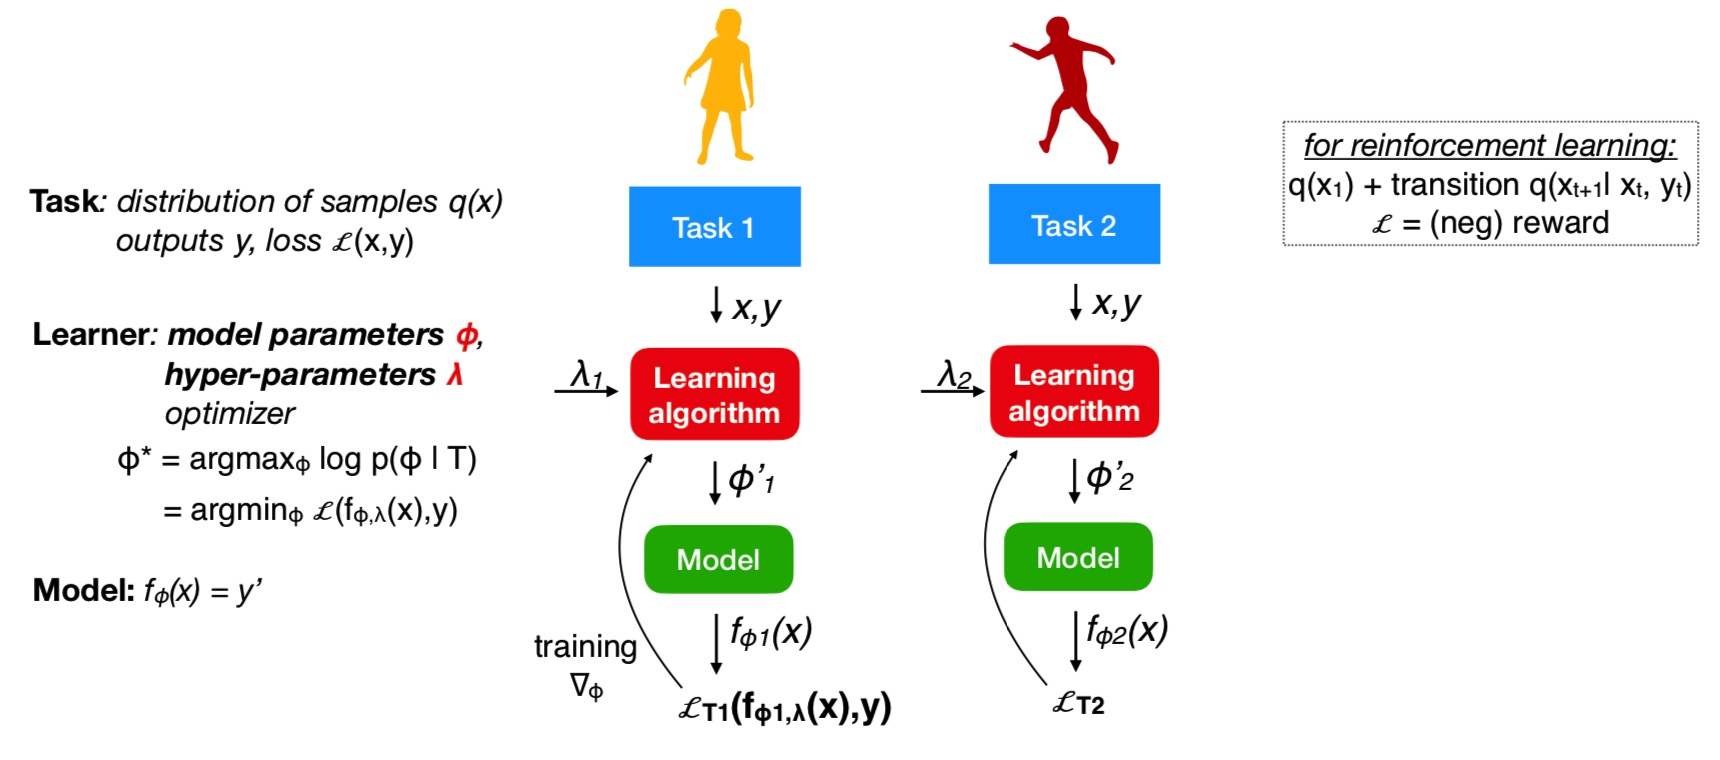
\includegraphics[height=6cm]{image/Jietu20220328-194743.jpg}

\end{frame}
\begin{frame}{Terminology}

\centering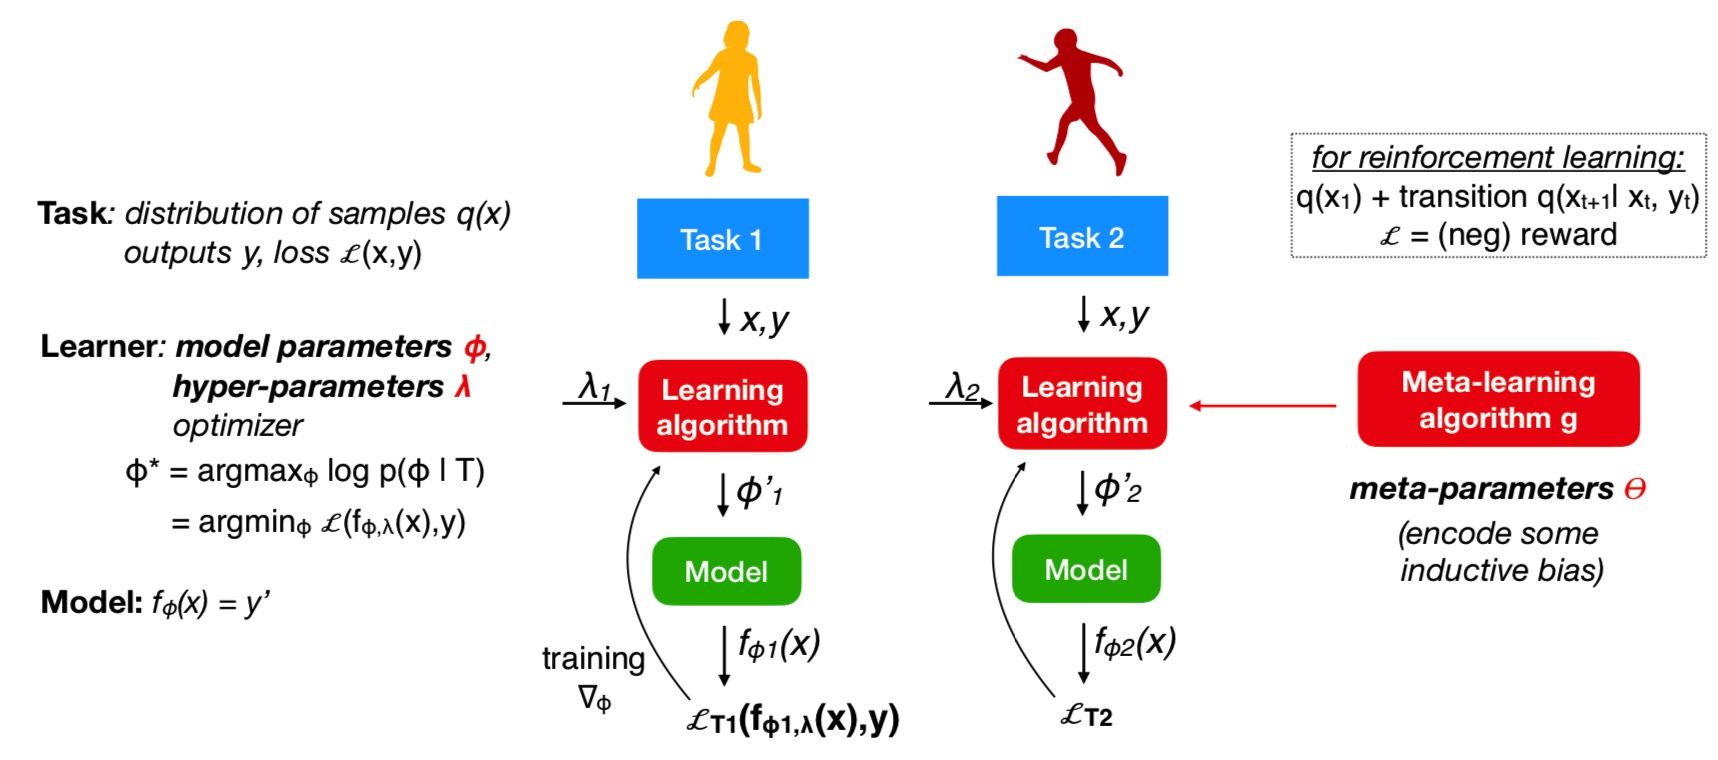
\includegraphics[height=6cm]{image/Jietu20220328-194806.jpg}

\end{frame}

\begin{frame}{Learning hyperparameters}
\centerline{Closely related to Automated Machine Learning (AutoML)}
\centerline{But:\textcolor{red}{meta-learn }how to design architectures/pipelines and tune hyperparameters}
\centerline{\textit{\textcolor{red}{Human data scientists also learn from experience}}}
\centering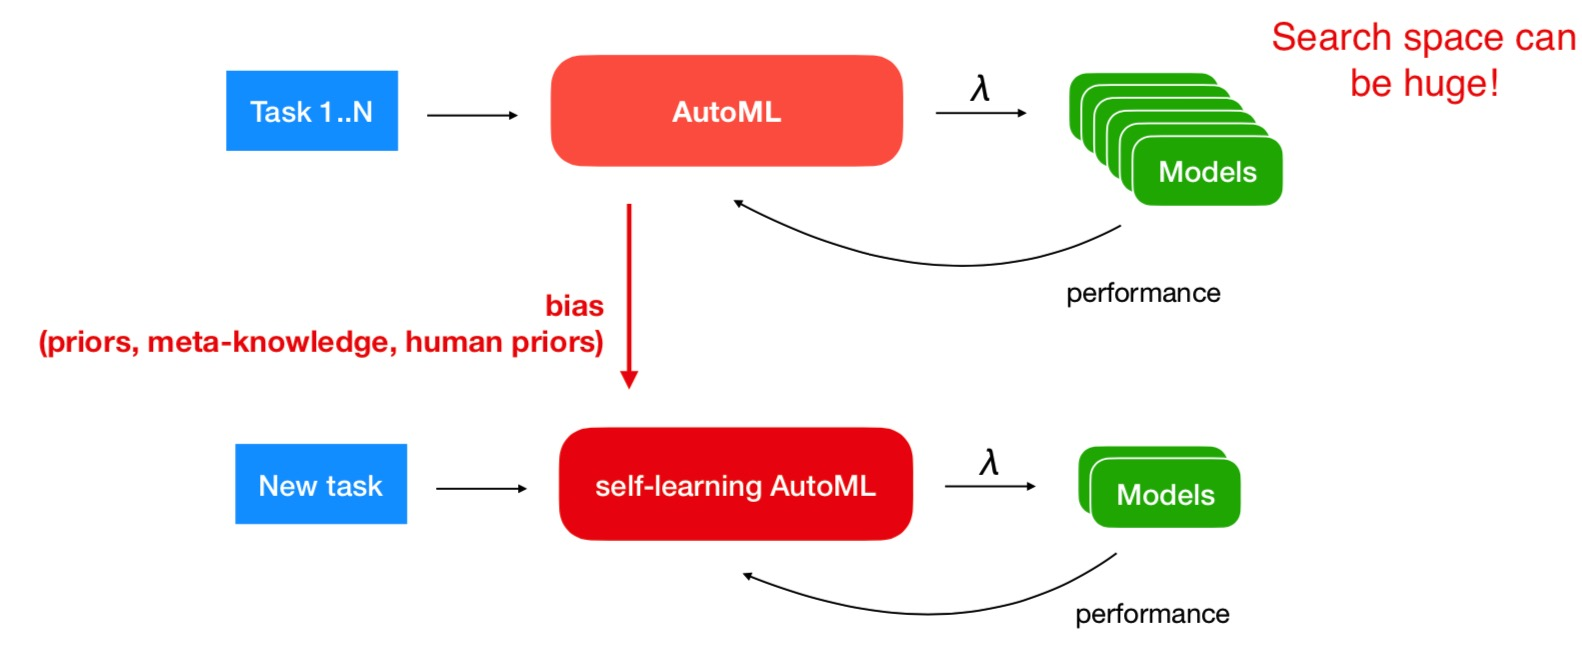
\includegraphics[height=5cm]{image/Jietu20220328-195244.jpg}
\end{frame}


\begin{frame}{Meta-learning for AutoML: how?}
\small\centerline{hyperparameters = architecture + hyperparameters}


\centering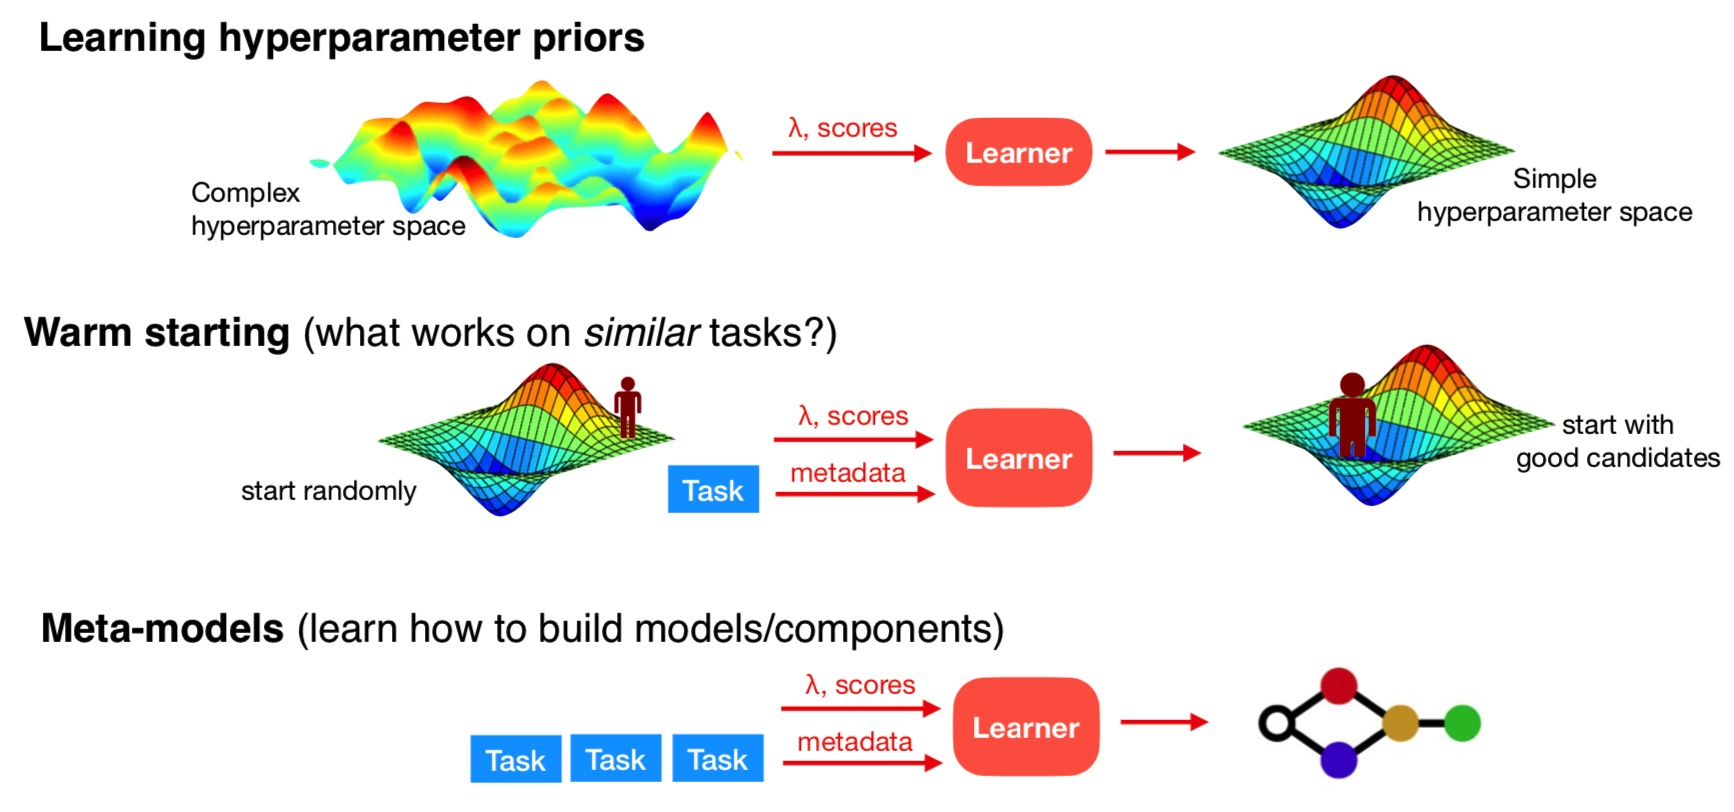
\includegraphics[height=6cm]{image/Jietu20220328-195525.jpg}

\end{frame}

\begin{frame}{Observation:}{current AutoML strongly depends on learned priors}

\centering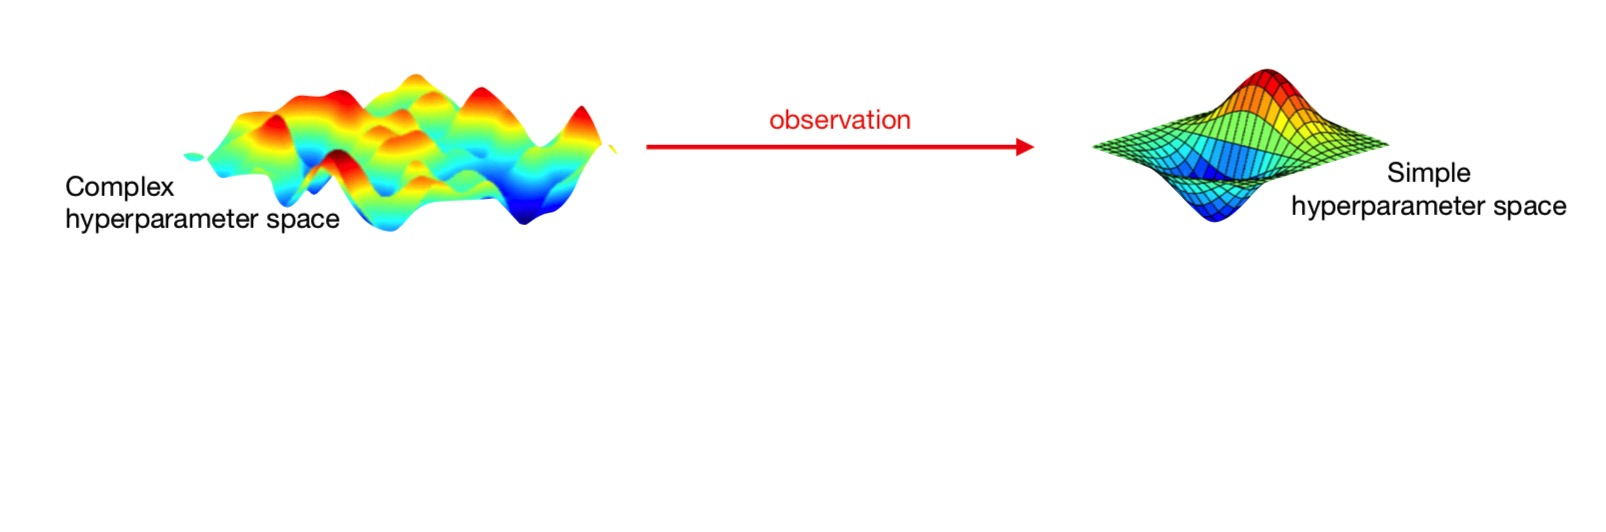
\includegraphics[height=5cm]{image/Jietu20220328-195740.jpg}

\end{frame}

\begin{frame}{Manual architecture priors}
\begin{itemize}
\item \textcolor{red}{Most successful pipelines have a similar structure}
\item \textcolor{red}{Can we meta-learn a prior over successful structures?} 
\end{itemize}


\centering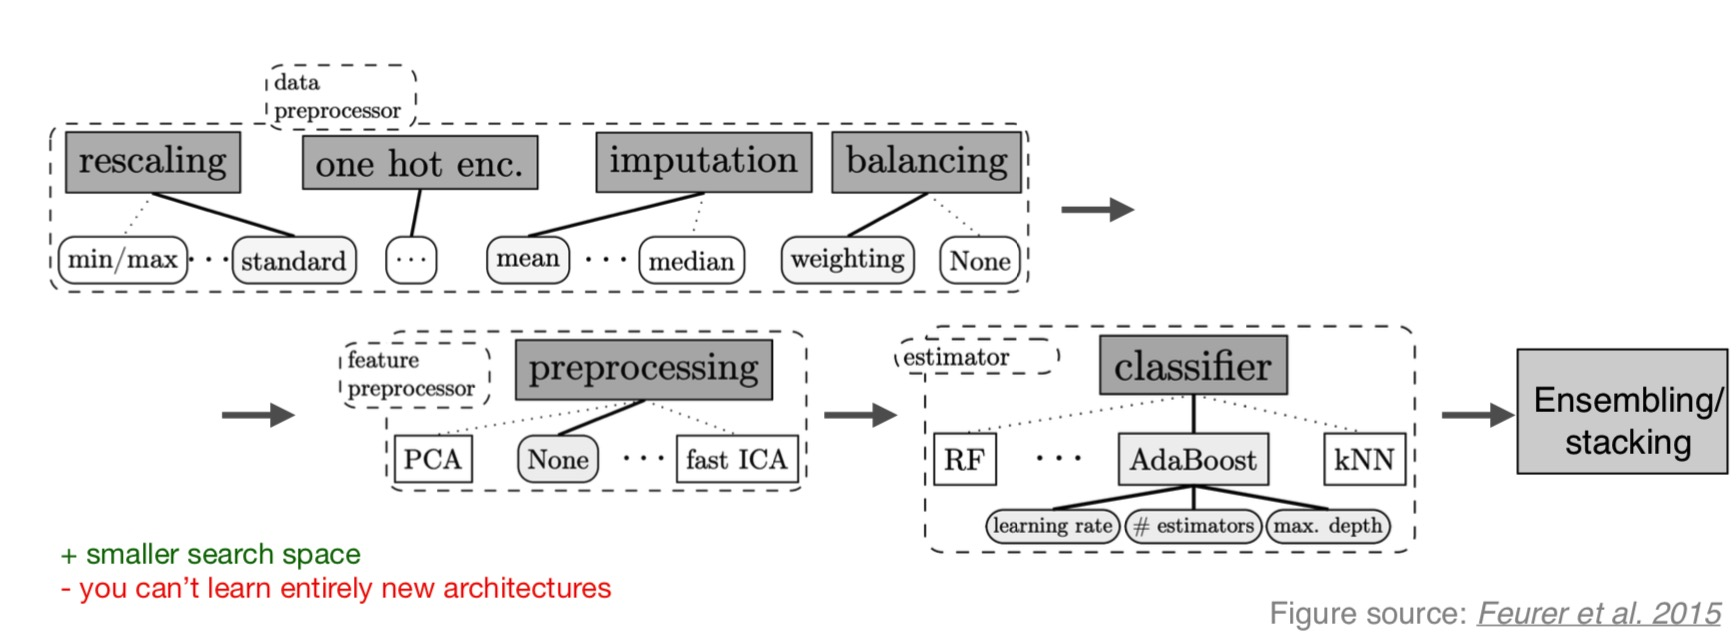
\includegraphics[height=5cm]{image/Jietu20220328-200135.jpg}

\end{frame}

\begin{frame}{Manual architecture priors}
\textcolor{red}{Successful deep networks often have repeated motifs (cells)}
\centering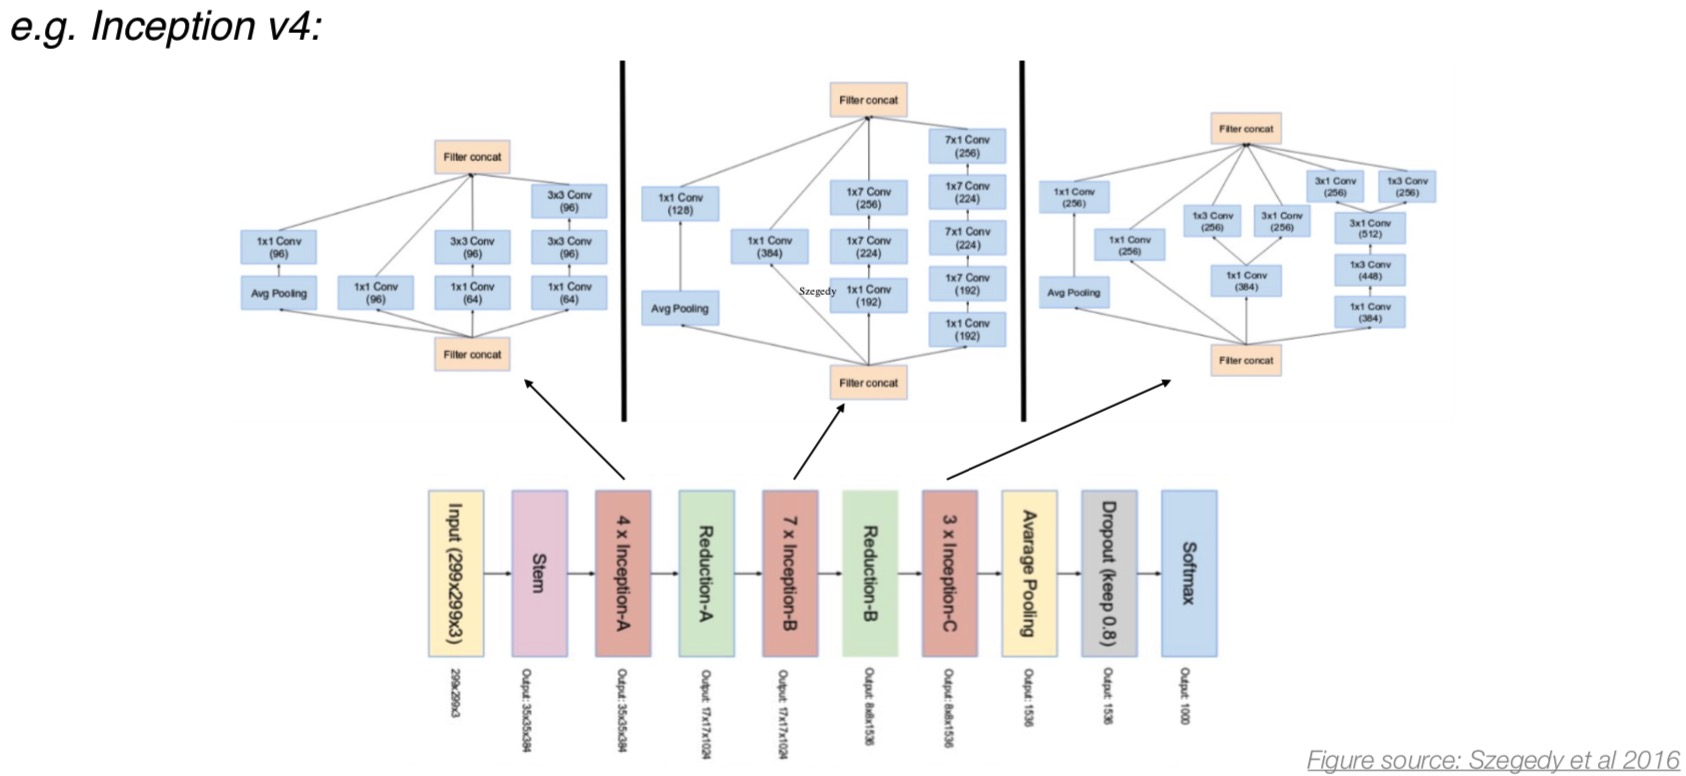
\includegraphics[height=6cm]{image/Jietu20220328-200331.jpg}

\end{frame}

\begin{frame}{Cell search space prior}

\centering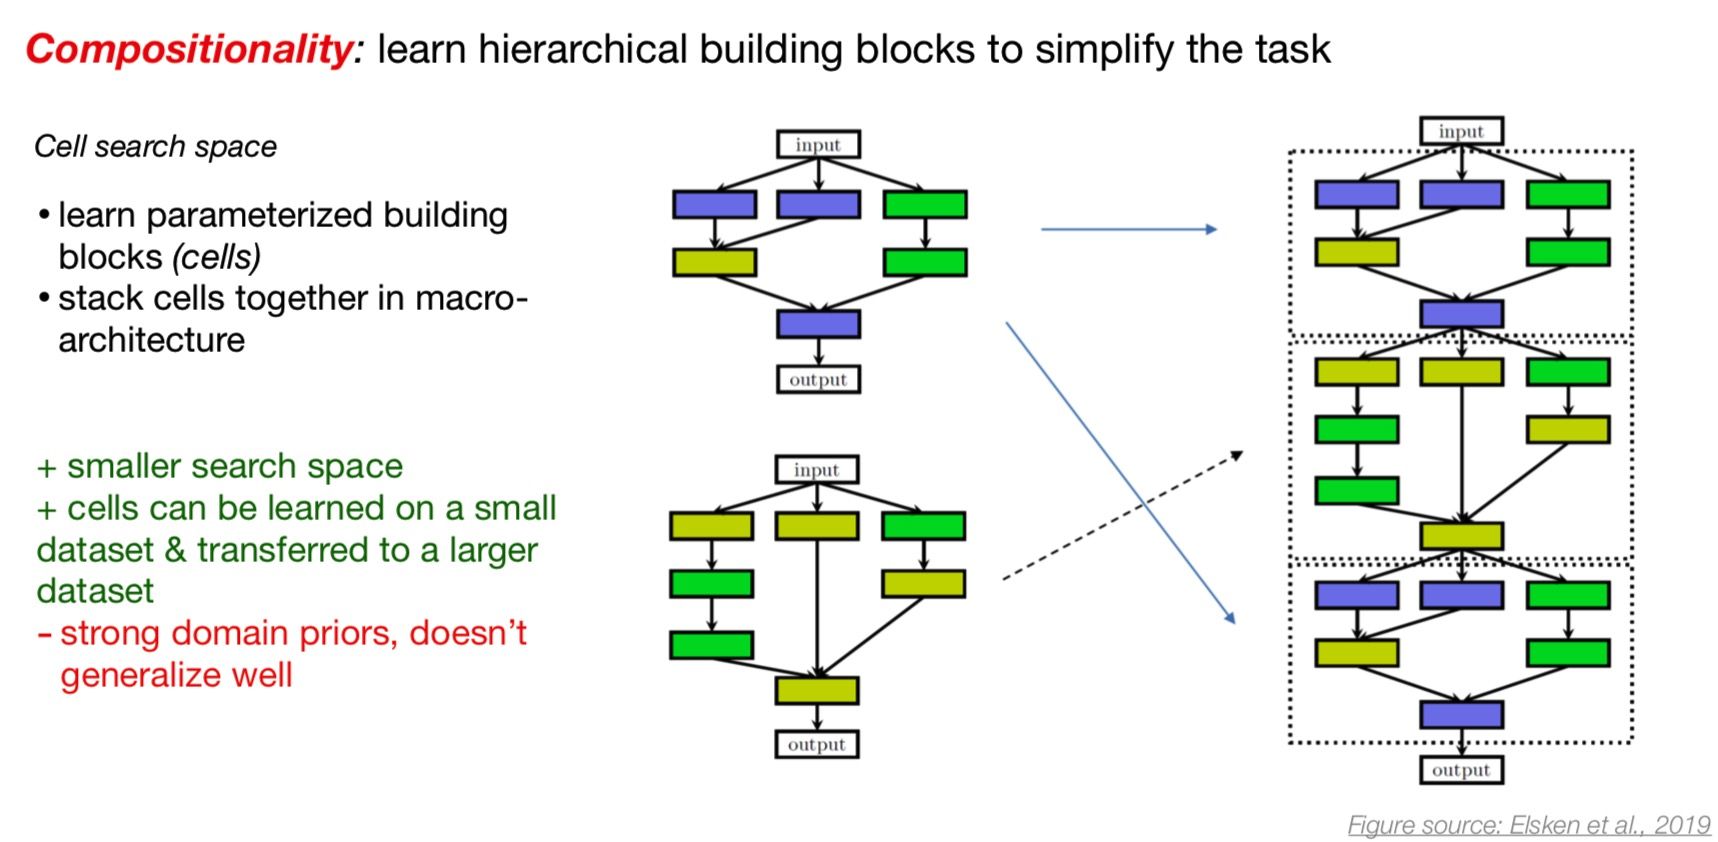
\includegraphics[height=6cm]{image/Jietu20220328-200520.jpg}
\pause
\\\small\textcolor{red}{Can we meta-learn hierarchies / components that generalize better?}

\end{frame}

\begin{frame}{Cell search space prior}

\centering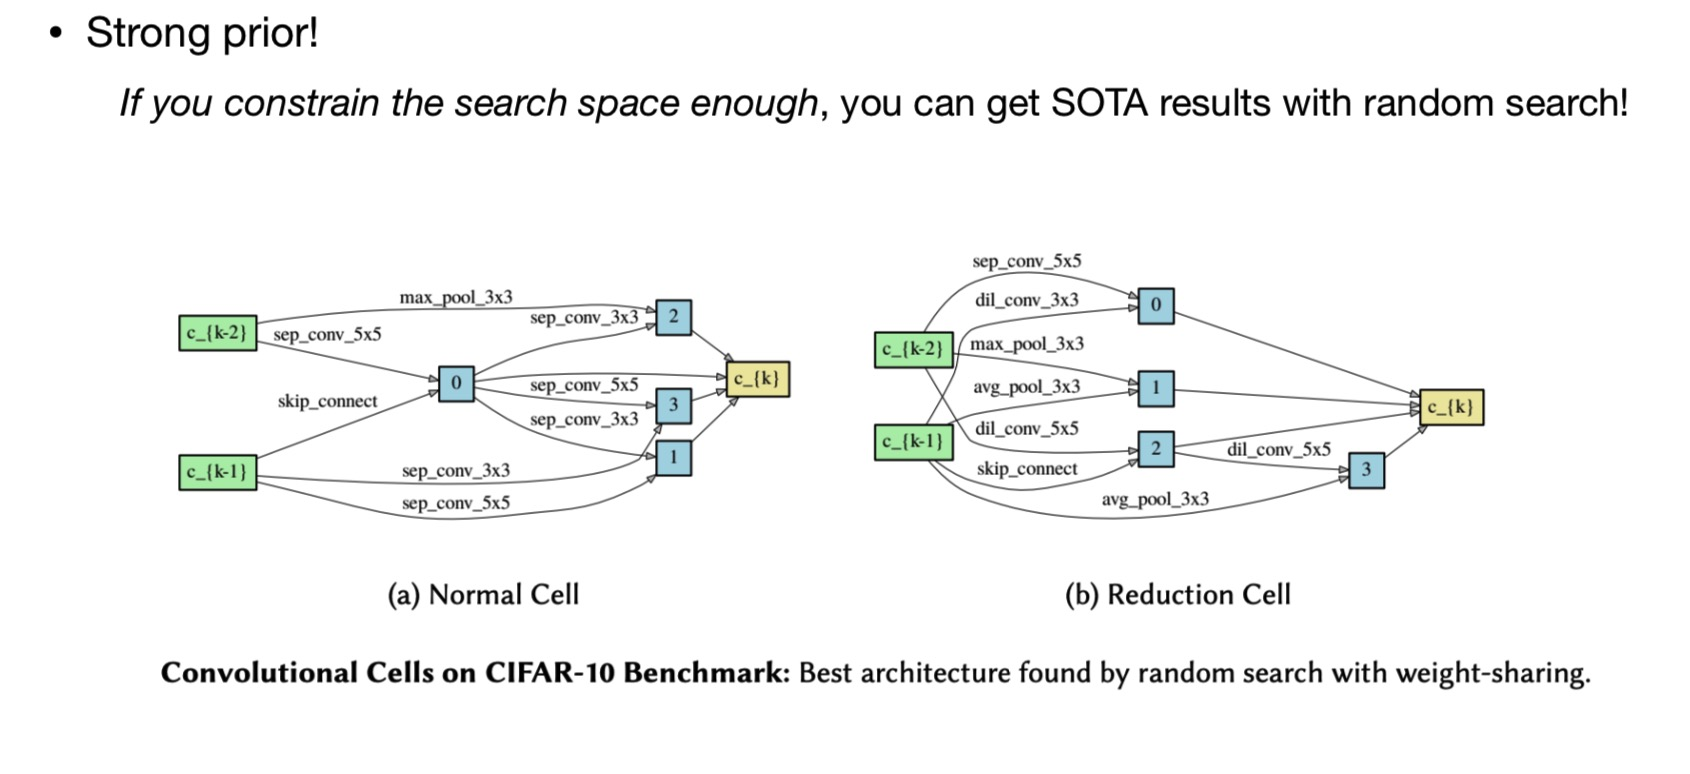
\includegraphics[height=7cm]{image/Jietu20220328-200717.jpg}


\end{frame}

\begin{frame}{Manual priors: Weight sharing}

\centering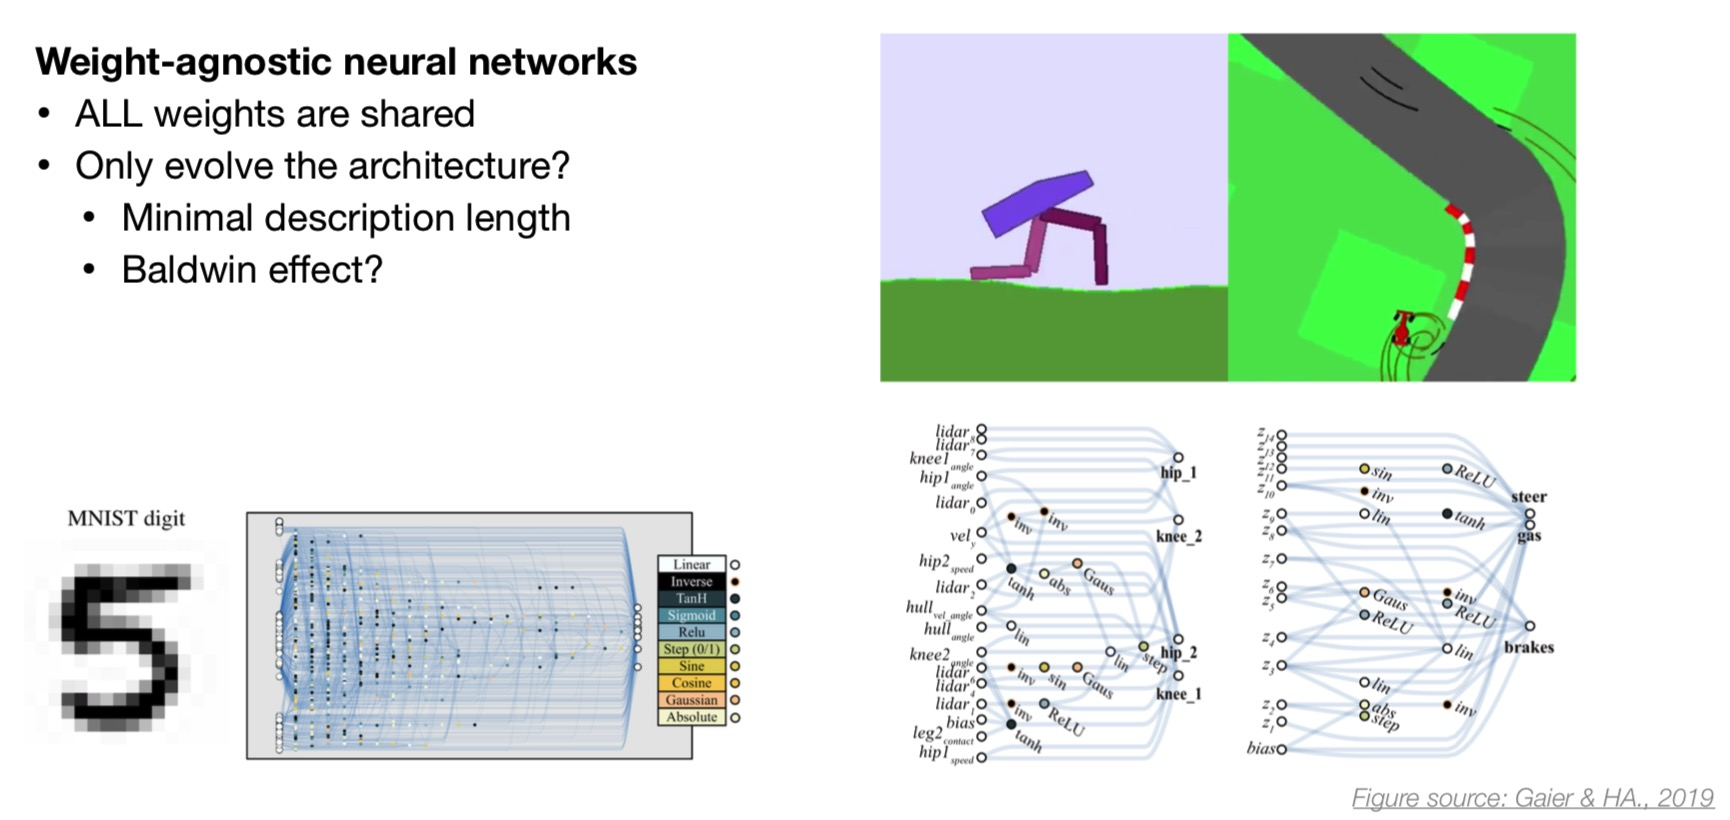
\includegraphics[height=7cm]{image/Jietu20220328-200845.jpg}


\end{frame}
\begin{frame}{Learning hyperparameter priors}

\centering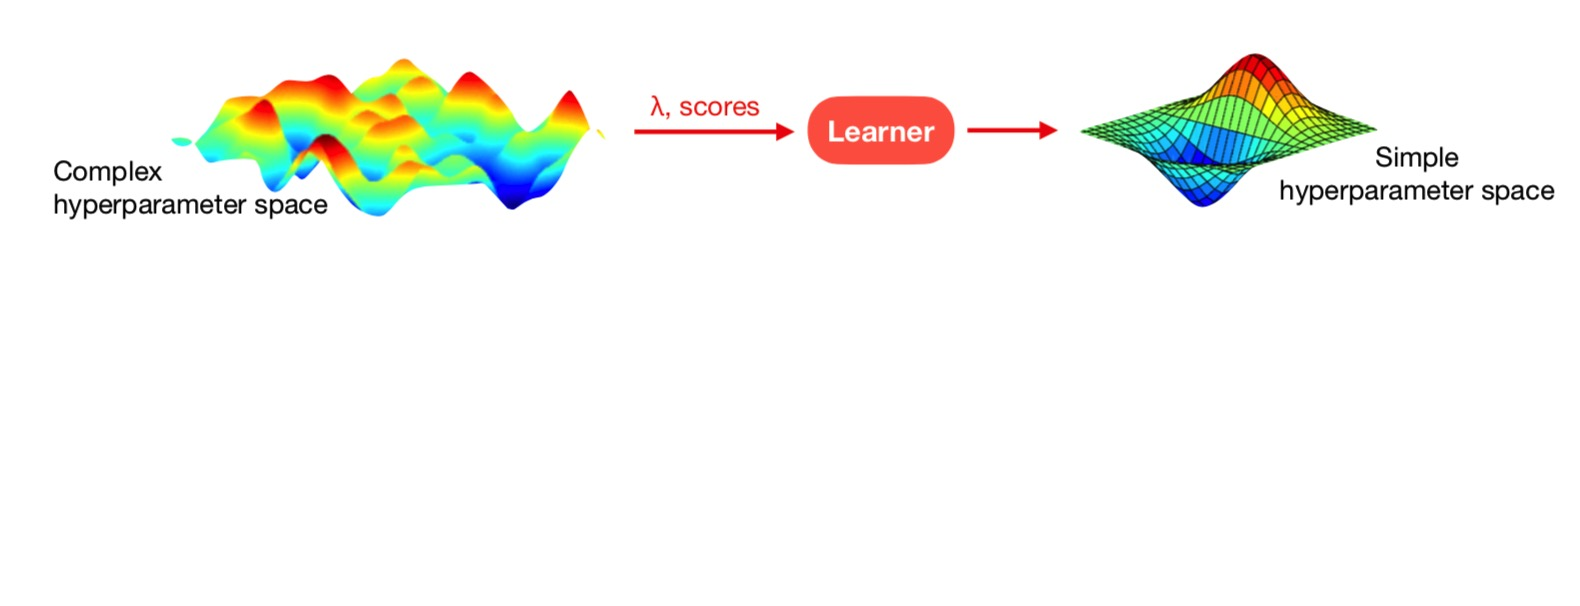
\includegraphics[height=5cm]{image/Jietu20220328-200954.jpg}


\end{frame}
\begin{frame}{Learn hyperparameter importance}

\centering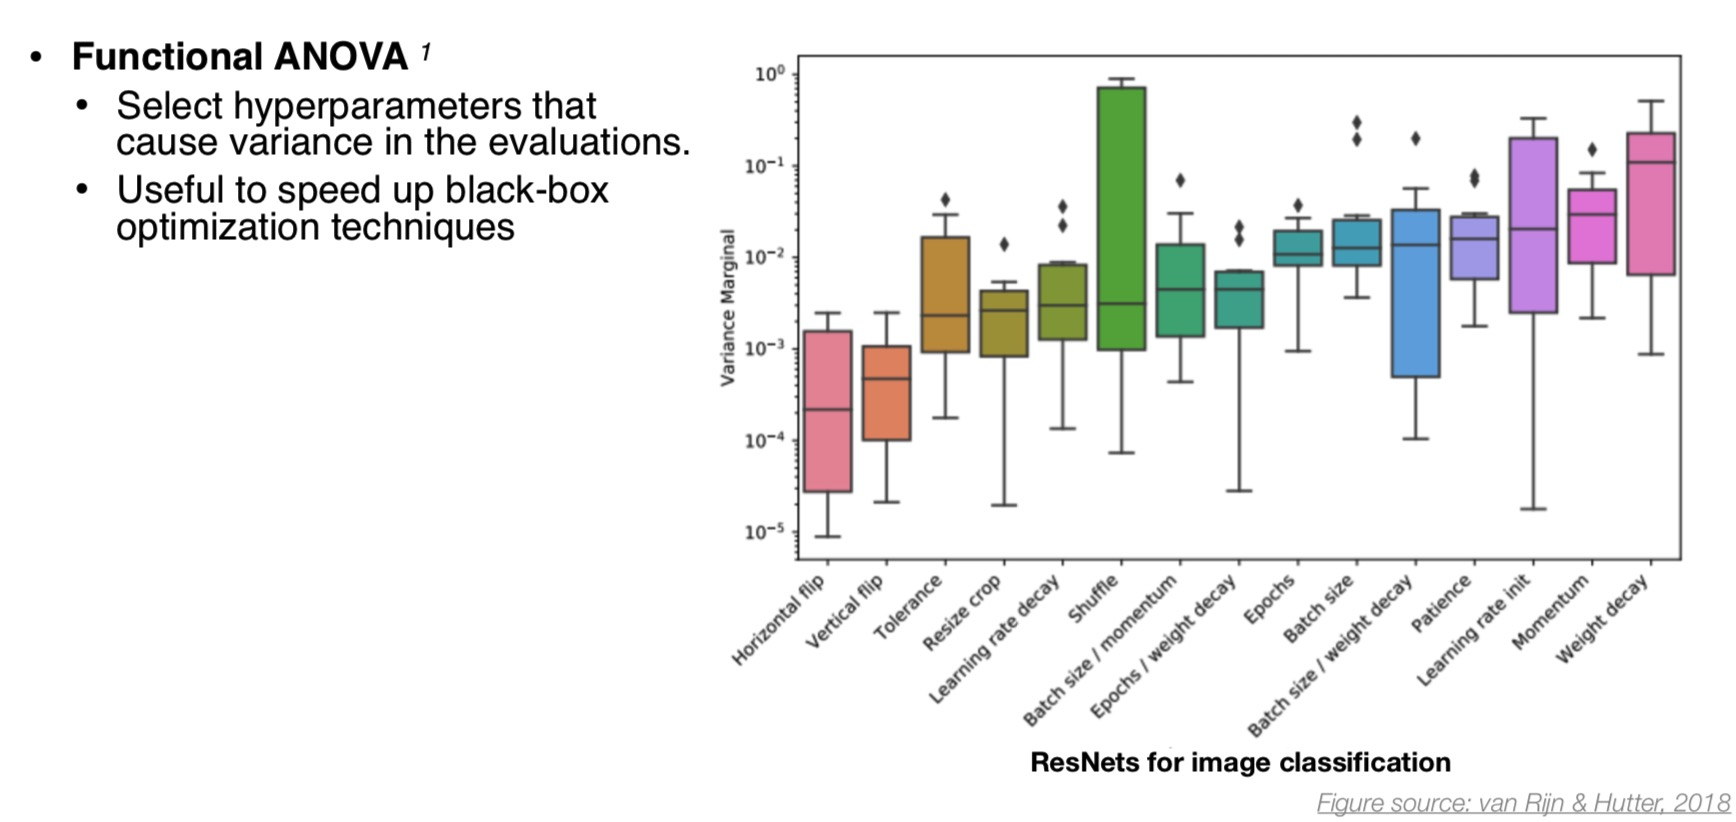
\includegraphics[height=6cm]{image/Jietu20220328-201111.jpg}


\end{frame}
\begin{frame}{Learn defaults + hyperparameter importance}

\begin{itemize}
    \item \textbf{Tunability} \\\textit{\textcolor{red}{Learn} good defaults, measure \textcolor{red}{importance} as improvement via tuning}
\end{itemize}
\centering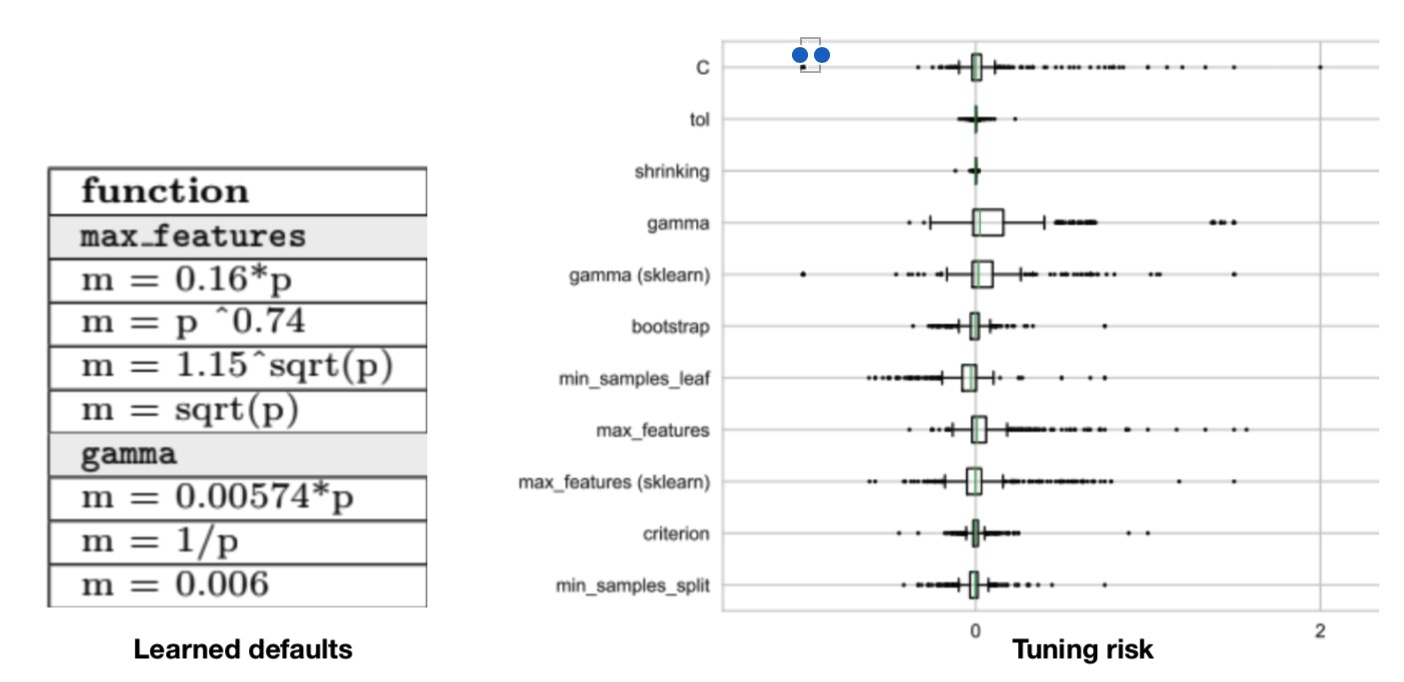
\includegraphics[height=5.5cm]{image/Jietu20220328-201428.jpg}


\end{frame}
\begin{frame}{Bayesian Optimization (interlude)}
\begin{itemize}
    \item Start with a few (random) hyperparameter configurations
    \item Fit a \textcolor{purple}{surrogate model}  to predict other configurations
    \item Probabilistic regression: mean $\mu$ and standard deviation $\sigma$ \textcolor{purple}{(blue band)}
    \item Use an \textcolor{green}{acquisition function }to trade off exploration and exploitation, e.g. Expected Improvement (EI)
    \item Sample for the best configuration under that function
\end{itemize}
\centering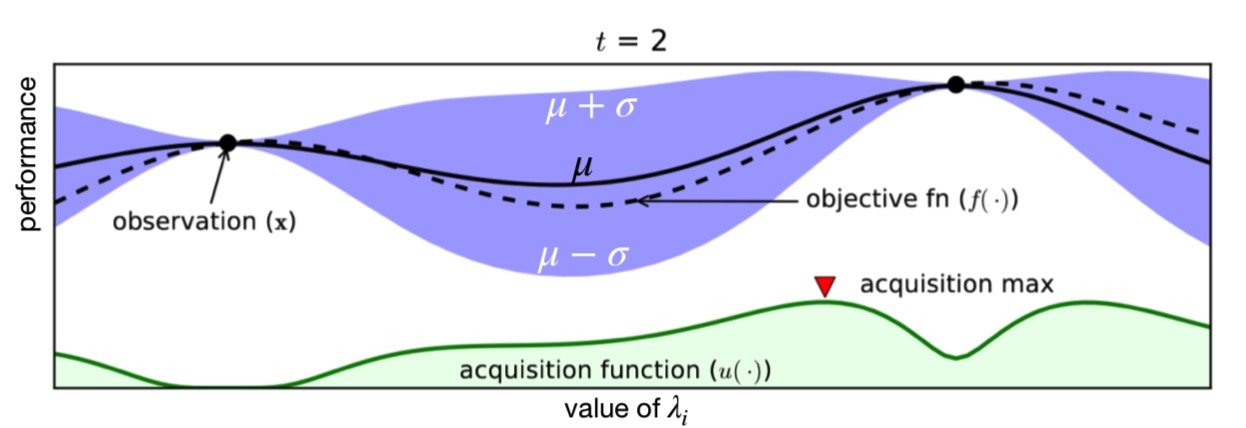
\includegraphics[height=3cm]{image/Jietu20220328-201705.jpg}


\end{frame}
\begin{frame}{Bayesian Optimization}

\begin{itemize}
    \item Repeat until some stopping criterion:
        \begin{itemize}
            \item Fixed budget
            \item Convergence
            \item EI threshold
        \end{itemize}
    \item Theoretical guarantees 
        \begin{itemize}
            \item \textit{Srinivas et al. 2010, Freitas et al. 2012, Kawaguchi et al. 2016}
        \end{itemize}
    \item Also works for non-convex, noisy data
    \item Used in AlphaGo
\end{itemize}

\end{frame}
\begin{frame}{Bayesian Optimization}

\centering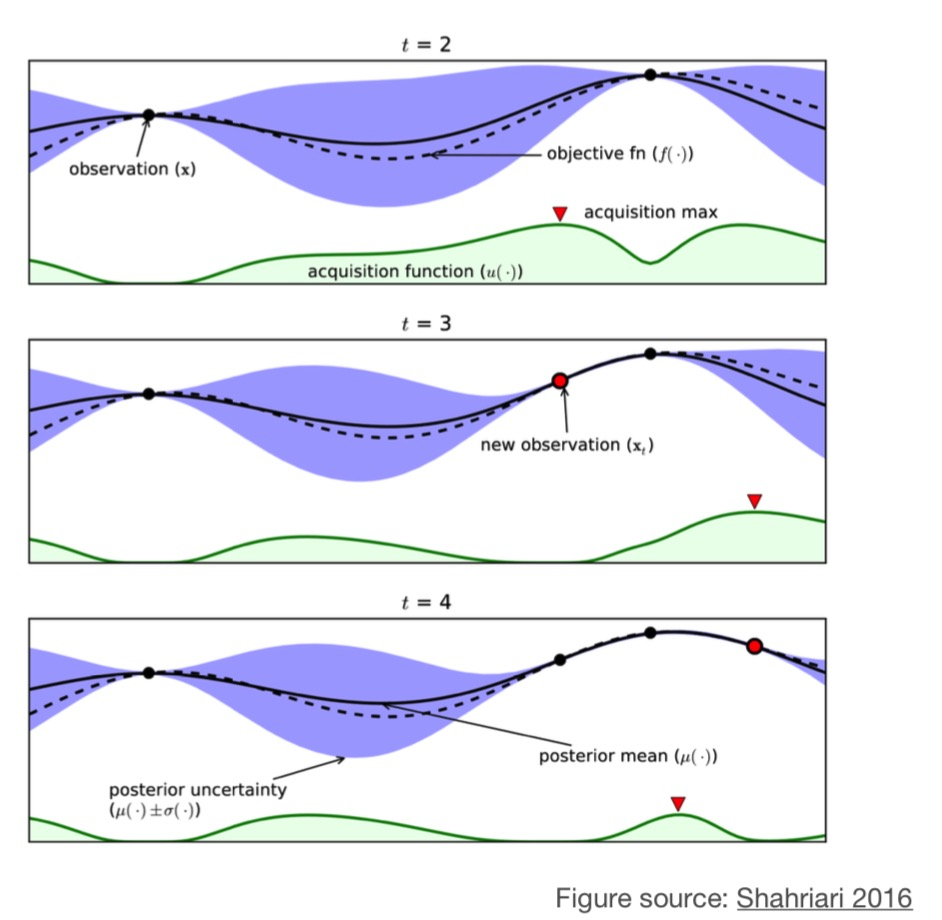
\includegraphics[height=7cm]{image/Jietu20220328-202037.jpg}


\end{frame}
\begin{frame}{Learn basis expansions for hyperparameters}

    \begin{itemize}
        \item Hyperparameters can interact in very non-linear ways
        \item Use a neural net to learn a suitable basis expansion $\phi _z(\lambda)$ for all tasks
        \item \textcolor{green}{You can use Bayesian linear models, transfers info on configuration space}
    \end{itemize}
\small \textcolor{blue}{Learn basis expansion on lots of data (e.g. OpenML)}
\centering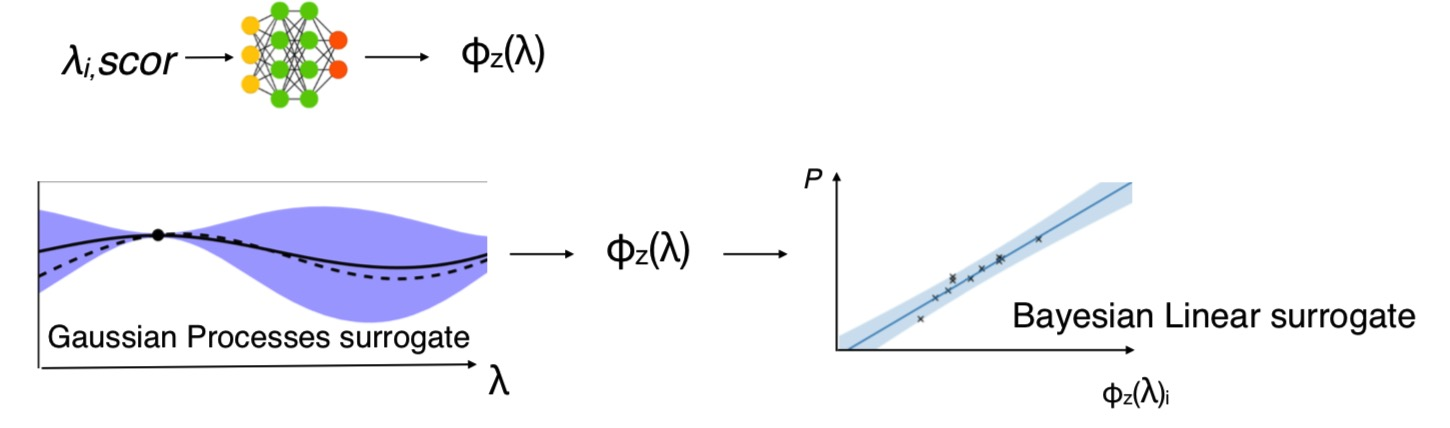
\includegraphics[height=4cm]{image/Jietu20220328-202530.jpg}

\end{frame}

\begin{frame}{Surrogate model transfer}
    \begin{itemize}
        \item If task $j$ is similar to the new task, its surrogate model $S_j$ will likely transfer well
        \item Sum up all $S_j$ predictions, weighted by task similarity (as in active testing)
        \item Build combined Gaussian process, weighted by current performance on new task
    \end{itemize}
\centering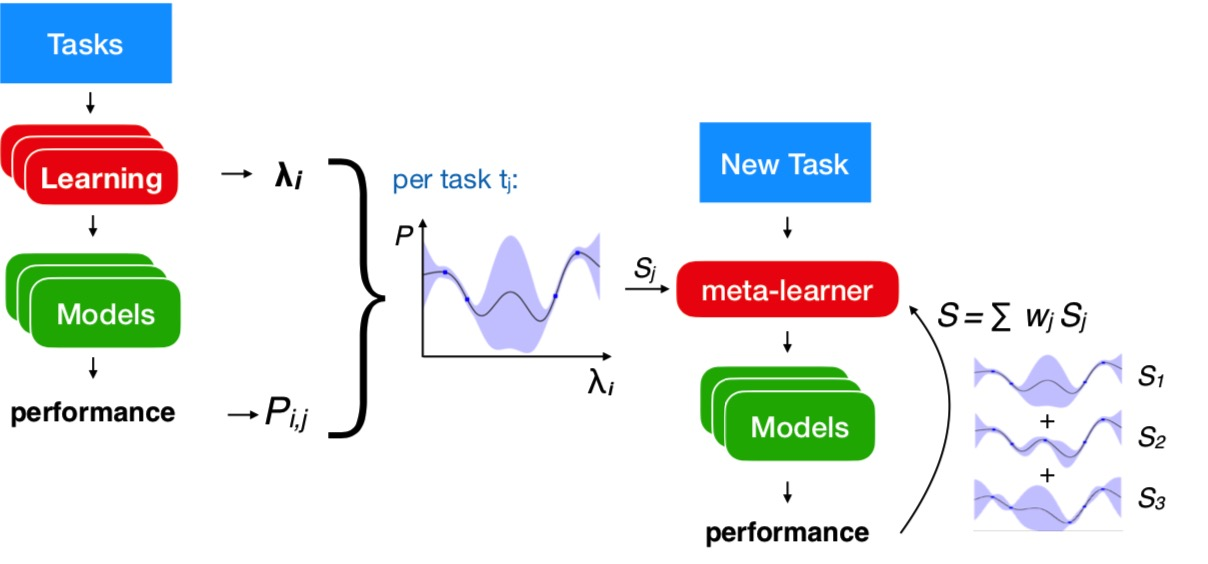
\includegraphics[height=6cm]{image/Jietu20220328-202917.jpg}

\end{frame}

\begin{frame}{Surrogate model transfer}
    \begin{itemize}
        \item Store surrogate model $S_ij$ for every pair of task $i$ and algorithm $j$
        \item \textcolor{red}{Simpler surrogates, better transfer}
        \item Learn weighted ensemble $\rightarrow $ significant speed up in optimization
    \end{itemize}
\centering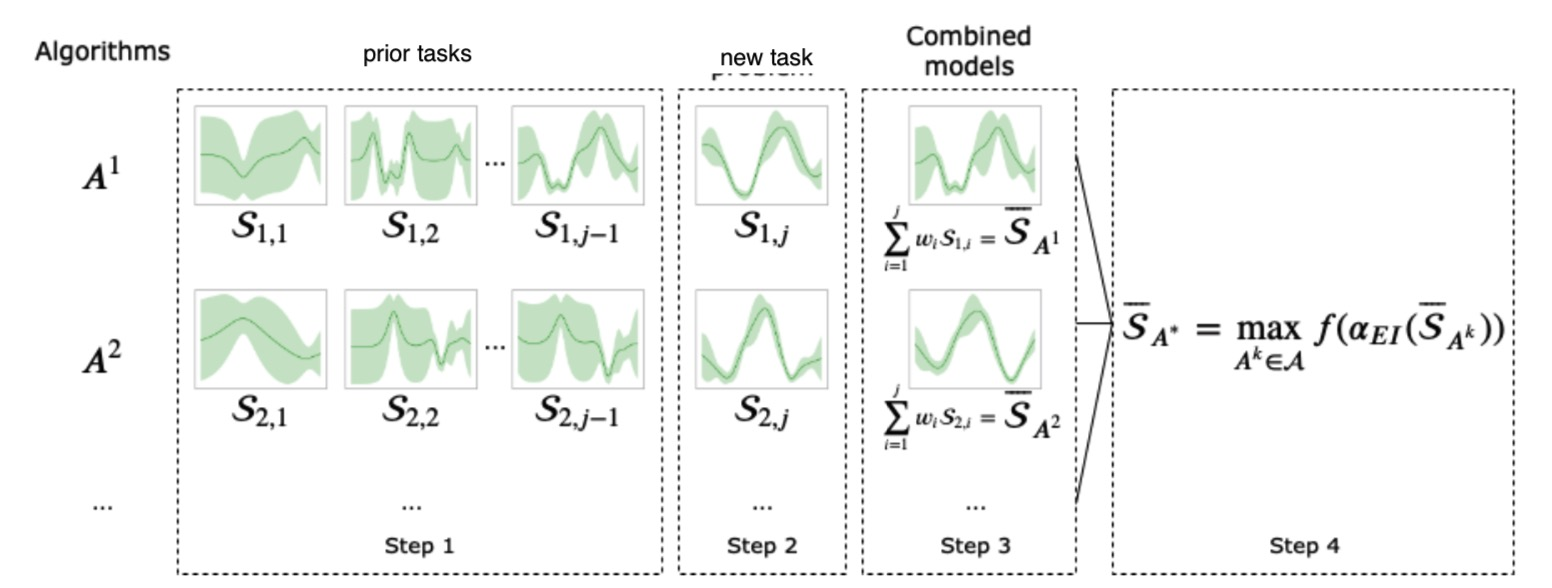
\includegraphics[height=5cm]{image/Jietu20220328-203139.jpg}

\end{frame}
\begin{frame}{Warm starting}{(what works on similar tasks?)}
    \centering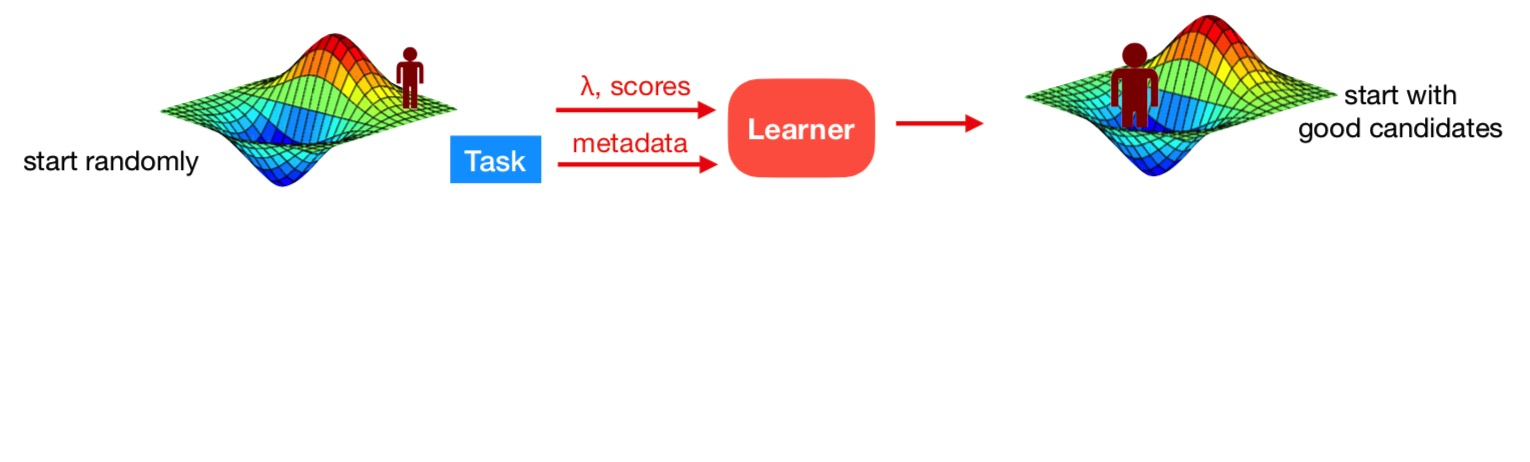
\includegraphics[height=4cm]{image/Jietu20220328-203410.jpg}
\end{frame}

\begin{frame}{How to measure task similarity?}
    \begin{itemize}
        \item Hand-designed (statistical) meta-features that describe (tabular) datasets
        \item Task2Vec: task embedding for image data
        \item Optimal transport: similarity measure based on comparing probability distributions
        \item Metadata embedding based on textual dataset description
        \item Dataset2Vec: compares batches of datasets
        \item Distribution-based invariant deep networks
    \end{itemize}
    \centering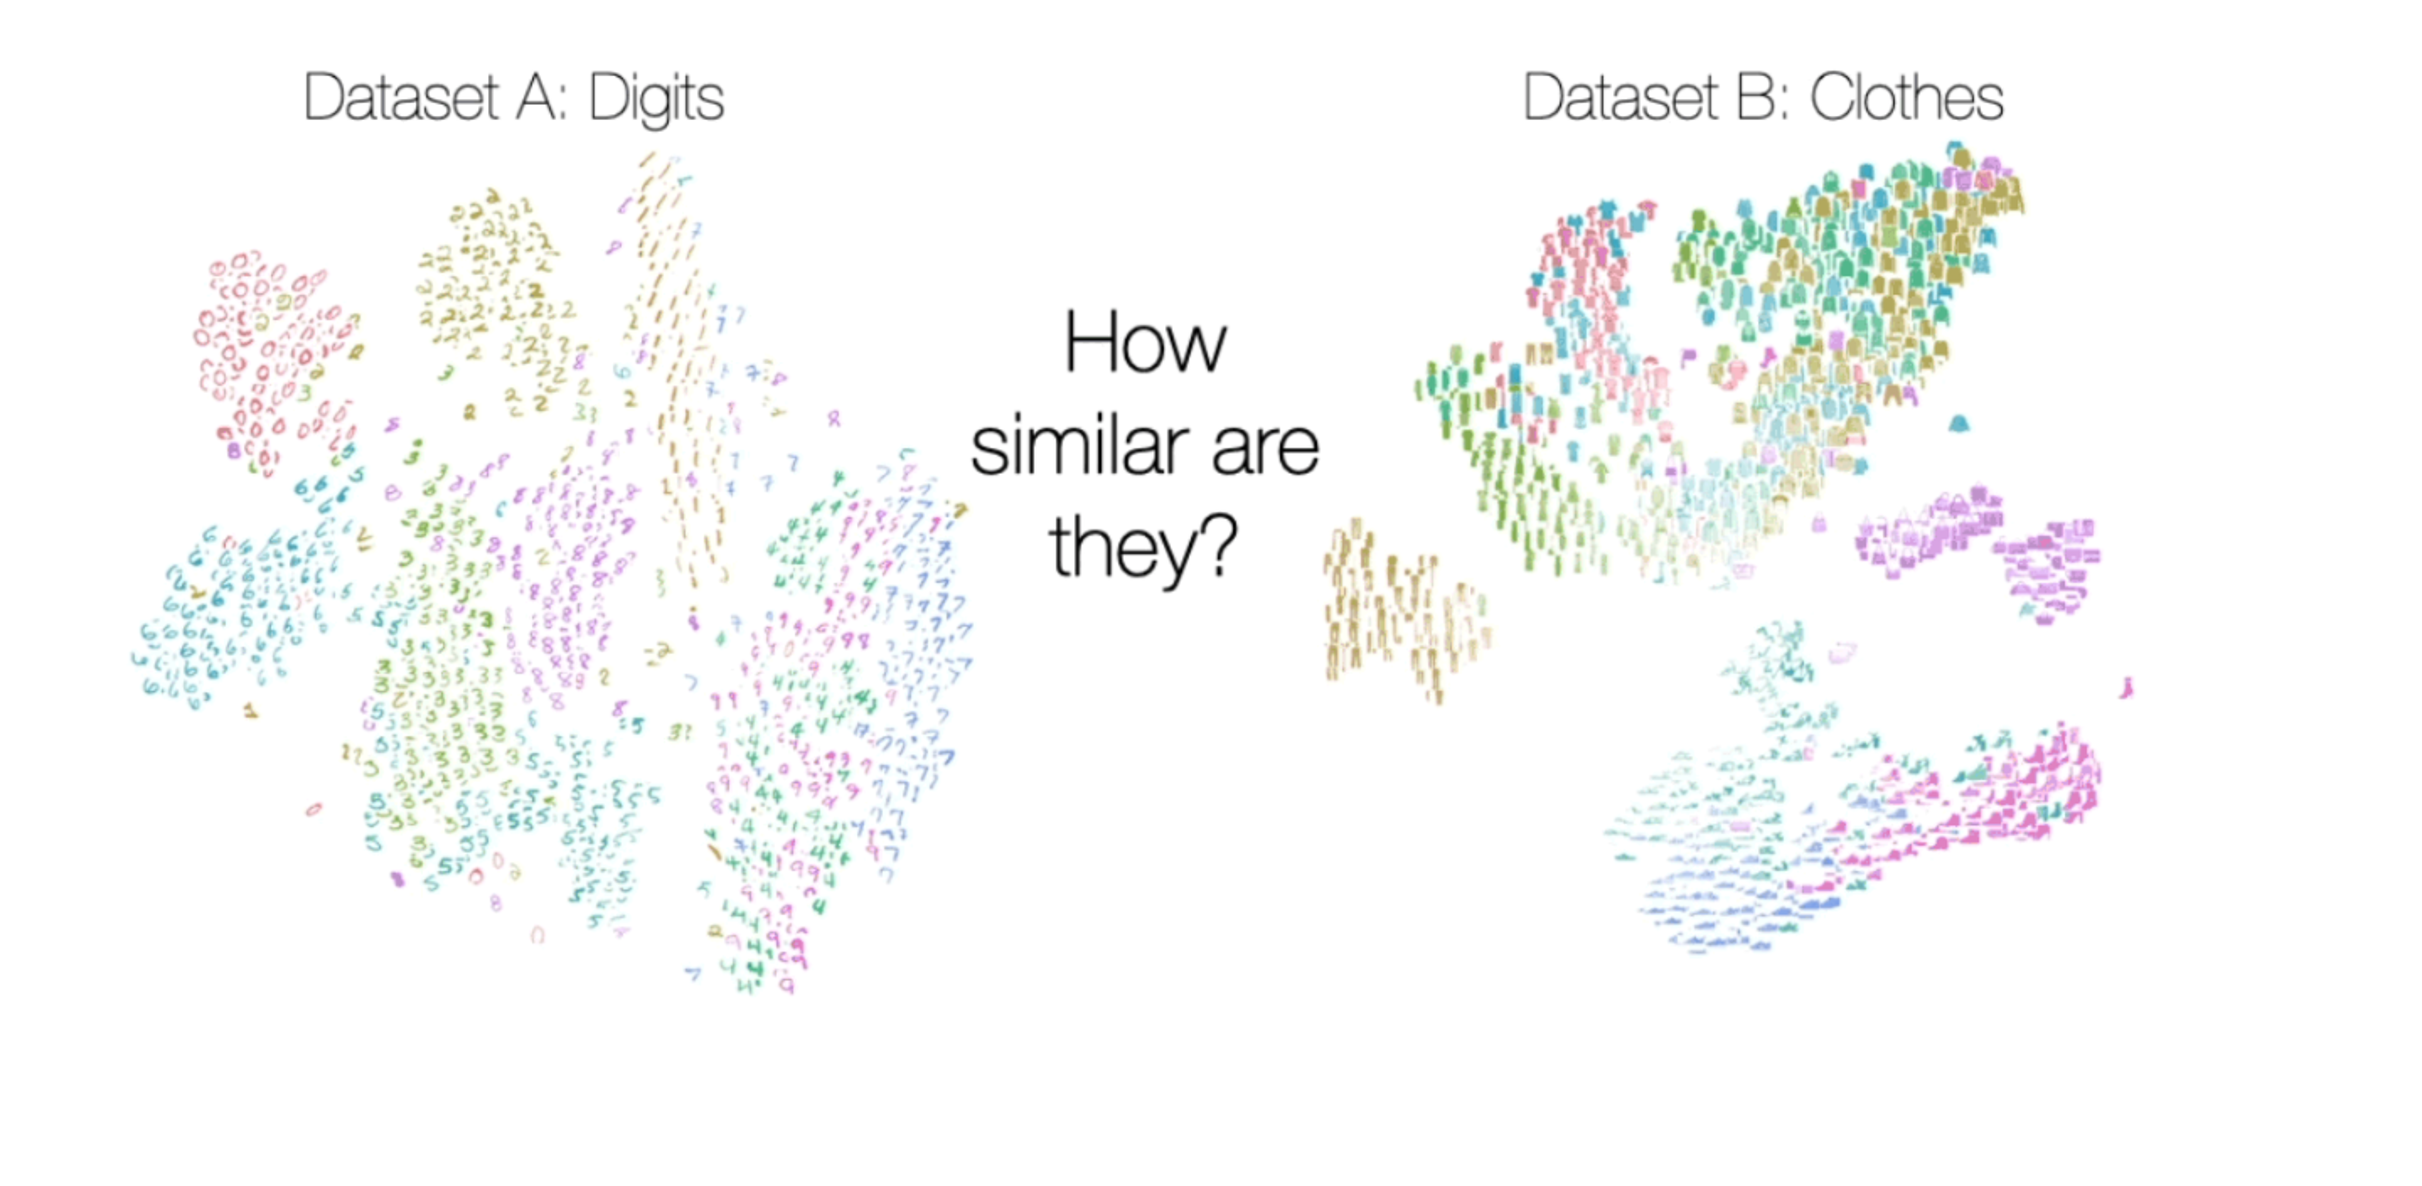
\includegraphics[height=5cm]{image/Picture1.png}
\end{frame}
\begin{frame}{Warm-starting with kNN}
    \begin{itemize}
        \item Find k most similar tasks, warm-start search with best $\lambda _i$
        \begin{itemize}
            \item Auto-sklearn: Bayesian optimization (SMAC)
            \begin{itemize}
                \item Meta-learning yield better models, faster
                \item Winner of AutoML Challenges
            \end{itemize}
        \end{itemize}
    \end{itemize}
    \centering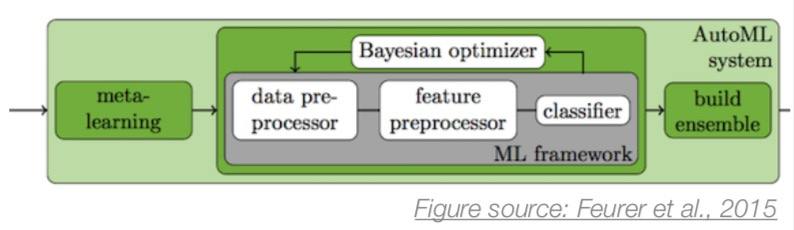
\includegraphics[height=3cm]{image/Jietu20220328-204247.jpg}
    
\end{frame}
\begin{frame}{Warm-starting with kNN}
    \centering\includegraphics[height=5cm]{image/Jietu20220328-204255.jpg}
\end{frame}
\begin{frame}{Probabilistic Matrix Factorization}
    \begin{itemize}
        \item Collaborative filtering: configurations $\lambda_i$ are `rated’ by tasks  $t_j$
        \item Learn  latent representation for tasks $T$ and configurations $\lambda$
        \item Use meta-features to warm-start on new task
        \item Returns probabilistic predictions for Bayesian optitmization

    \end{itemize}
    \centering\includegraphics[height=5cm]{image/Jietu20220328-204634.jpg}
\end{frame}

\begin{frame}{DARTS: Differentiable NAS}
    \begin{itemize}
        \item Fixed (one-shot) structure, learn which operators to use
        \item Give all operators a weight $\alpha_i$
        \item Optimize $\alpha_i$ and model weights $\omega_j$ using bilevel optimization
        \begin{itemize}
            \item approximate $\omega_j*(\alpha_i)$ adapting $\omega_j$ after every training step
        \end{itemize}
    \end{itemize}
    \centering\includegraphics[height=5cm]{image/Picture2.png}
\end{frame}

\begin{frame}{Warm-started DARTS}
    \begin{itemize}
        \item Warm-start DARTS with architectures that worked well on similar problems
        \item Slightly better performance, but much faster (5x)
    \end{itemize}
    \centering\includegraphics[height=5cm]{image/Picture3.png}
\end{frame}

\begin{frame}{Meta-models}
    (learn how to build models/components)
    \centering\includegraphics[height=3cm]{image/Jietu20220328-233402.jpg}
\end{frame}

\begin{frame}{Algorithm selection models}
    \centering\includegraphics[height=7cm]{image/Jietu20220328-233552.jpg}
\end{frame}

\begin{frame}{Learning model components}
    \begin{itemize}
        \item Learn nonlinearities: RL-based search of space of likely useful activation functions 
        \begin{itemize}
            \item E.g. \textit{Swish} can outperform ReLU
            $$  \text { Swish: } \frac{x}{1+e^{-\beta x}}$$
        \end{itemize}
        \item Learn optimizers: RL-based search of space of likely useful update rules 
        \begin{itemize}
            \item E.g. PowerSign can outperform Adam, RMPprop
            \item PowerSign $: e^{\operatorname{sign}(g) \operatorname{sign}(m)} g$
g: gradient, m:moving average
        \end{itemize}
        \item Learn acquisition functions for Bayesian optimization
    \end{itemize}
    \includegraphics[height=3cm]{image/Jietu20220328-234610.jpg}
    \includegraphics[height=3cm]{image/Jietu20220328-234631.jpg}
\end{frame}

\begin{frame}{Monte Carlo Tree Search + reinforcement learning}
    \begin{itemize}
        \item \textbf{\textit{Self-play:}}
        \begin{itemize}
            \item Game actions: insert, delete, replace components in a pipeline
            \item Monte Carlo Tree Search builds pipelines given action probabilities
            \begin{itemize}
                \item With grammar to avoid invalid pipelines
            \end{itemize}
            \item Neural network (LSTM) Predicts pipeline performance (can be pre-trained on prior datasets)
        \end{itemize}
    \end{itemize}
    \centering\includegraphics[height=5cm]{image/Jietu20220328-235128.jpg}
\end{frame}
\begin{frame}{Meta-Reinforcement Learning for NAS}
    Results on increasingly difficult tasks:
    \begin{itemize}
        \item Initially slower than DQN, but faster after a few tasks
        \item Policy entropy shows learning/relearning
    \end{itemize}
    \includegraphics[height=3cm]{image/Picture4.png}
    \includegraphics[height=3cm]{image/Picture5.png}
\end{frame}

\begin{frame}{MetaNAS: MAML + Neural Architecture Search}
    \begin{itemize}
        \item Combines gradient based meta-learning (REPTILE) with NAS
        \item During meta-train, it optimizes the meta-architecture (DARTS weights) along with the meta-parameters (initial weights) $\theta$
        \item During meta-test, the architecture can be adapted to the novel task through gradient descent
    \end{itemize}
    \centering\includegraphics[height=4cm]{image/Jietu20220328-235920.jpg}
\end{frame}


\begin{frame}{What can we learn to learn?}
    \centerline{\textit{3 pillars}}
    \centering\includegraphics[height=5.5cm]{image/Jietu20220329-000132.jpg}
\end{frame}

\begin{frame}{Terminology (reminder)}
    \centering\includegraphics[height=5.5cm]{image/Jietu20220329-000340.jpg}
\end{frame}

\begin{frame}{Strategy 1: bilevel optimization}

    \centerline{\textcolor{red}{parameterize some aspect of the learner that we want to learn as}} 
    \centerline{\textcolor{red}{meta-parameters $\theta$ meta-learn $\theta$ across tasks}}
    \centering\includegraphics[height=5cm]{image/Jietu20220329-000908.jpg}
    \small\centerline{$\Theta(Prior)$, could encode an initialization $\phi$, the hyperparameters $\lambda$, the optimizer,...}
    \leavevmode\hphantom{ }

    \small\centerline{\textit{Learned $\theta^*$ should \textcolor{blue}{learn $T_{new}$ from small amount of data, yet generalize to a large number of tasks}}}
\end{frame}

\begin{frame}{Meta-learning with bilevel optimization}
    \centering\includegraphics[height=7cm]{image/Jietu20220329-002035.jpg}
\end{frame}
\begin{frame}{Strategy 2: black-box models}

    \centerline{\textit{\textcolor{red}{black box meta-model $g_\theta$ predicts $\phi$ given $D_{train}$ ($theta$ is hidden)}}}
    \centerline{\textit{\textcolor{red}{hypernetwork where input embedding learned across tasks}}}
    \centering\includegraphics[height=6cm]{image/Jietu20220329-002812.jpg}
\end{frame}

\begin{frame}{Example: few-shot classification}
    \centering\includegraphics[height=6.5cm]{image/Jietu20220329-003052.jpg}
\end{frame}

\begin{frame}{Example: few-shot classification}
    \centering\includegraphics[height=6.5cm]{image/Jietu20220329-003340.jpg}
\end{frame}

\begin{frame}{Example: meta-reinforcement learning}
    \centering\includegraphics[height=7cm]{image/Jietu20220329-003718.jpg}
\end{frame}

\begin{frame}{Example: meta-reinforcement learning}
    \centering\includegraphics[height=7cm]{image/Jietu20220329-004129.jpg}
\end{frame}

\begin{frame}{Taxonomy of meta-learning methods}
    \small like base-learners, meta-learners consist of a representation, an objective, and an optimizer
    \centering\includegraphics[height=7cm]{image/Jietu20220329-004512.jpg}
\end{frame}


\begin{frame}{Taxonomy of meta-learning methods}
    \small like base-learners, meta-learners consist of a representation, an objective, and an optimizer
    \centering\includegraphics[height=7cm]{image/Jietu20220329-004703.jpg}
\end{frame}


\begin{frame}{Taxonomy of meta-learning methods}
    \small like base-learners, meta-learners consist of a representation, an objective, and an optimizer
    \centering\includegraphics[height=7cm]{image/Jietu20220329-004820.jpg}
\end{frame}
\begin{frame}{Gradient-based methods: learning $\phi_{init}$}
    \centering\includegraphics[height=7cm]{image/Jietu20220329-005015.jpg}
\end{frame}
\begin{frame}{Model agnostic meta-learning (MAML)}
    \centering\includegraphics[height=7cm]{image/Jietu20220329-005114.jpg}
\end{frame}
\begin{frame}{Model agnostic meta-learning (MAML)}
    \centering\includegraphics[height=7cm]{image/Jietu20220329-005224.jpg}
\end{frame}
\begin{frame}{Model agnostic meta-learning (MAML)}
    \centering\includegraphics[height=7cm]{image/Jietu20220329-005323.jpg}
\end{frame}
\begin{frame}{Model agnostic meta-learning (MAML)}
    Example of reinforcement learning:
    \begin{itemize}
        \item Goal: reach certain velocity in certain direction
    \end{itemize}
    \centering\includegraphics[height=5cm]{image/Jietu20220329-005513.jpg}
\end{frame}
\begin{frame}{Other gradient-based techniques}
    \centering\includegraphics[height=7cm]{image/Jietu20220329-005754.jpg}
\end{frame}
\begin{frame}{Scalability}
    \centering\includegraphics[height=6cm]{image/Jietu20220329-010316.jpg}
\end{frame}
\begin{frame}{Generalizability}
    \centering\includegraphics[height=7cm]{image/Jietu20220329-010613.jpg}
\end{frame}
\begin{frame}{Bayesian meta-learning}
    \centerline{Can meta-learning reason about \textcolor{red}{uncertainty} in the task distribution?}
    \centering\includegraphics[height=6cm]{image/Jietu20220329-010856.jpg}
\end{frame}
\begin{frame}{Fully Bayesian meta-learning}
    \centering\includegraphics[height=7cm]{image/Jietu20220329-011307.jpg}
\end{frame}
\begin{frame}{Meta-learning optimizers}
    Our brains probably don’t do backprop, instead:
    \begin{itemize}
        \item weights: networks that continuously modify the weights of another network
        \item Gradient based: parameterize the update rule using a neural network
        \begin{itemize}
            \item Learn meta-parameters across tasks, by gradient descent
            \centering\includegraphics[height=3cm]{image/Jietu20220329-011721.jpg}
        \end{itemize}
        \item Represent update rule as an LSTM, hierarchical RNN 
    \end{itemize}
\end{frame}
\begin{frame}{Meta-learning optimizers}
    \begin{itemize}
        \item Meta-learned (RNN) optimizers ‘rediscover’ momentum, gradient clipping, learning rate schedules, learning rate adaptation,… \\
        \item RL-based optimizers: represent updates as a policy, learn using guided policy search 
        \item Combined with MAML: 
        \begin{itemize}
            \item learn per-parameter learning rates
            \item learn precondition matrix (to `warp' the loss surface)
        \end{itemize}
        \item Black-box optimizers: meta-learned with an RNN, or with user-defined priors
        \item Speed up backpropagation by meta-learning sparsity and weight sharing 
    \end{itemize}
    \centering\includegraphics[height=3cm]{image/Jietu20220329-012318.jpg}
\end{frame}
\begin{frame}{Metric learning}

    \centerline{\textit{\textcolor{red}{Learn an embedding network $theta$ that transforms data ${D_{train},D_{test}}$ across all}}}
    \centerline{\textit{\textcolor{red}{tasks to a representation that allows easy similarity comparison}}}
    \centering\includegraphics[height=6cm]{image/Jietu20220329-012823.jpg}
\end{frame}
\begin{frame}{Prototypical networks}
    \centering\includegraphics[height=7cm]{image/Jietu20220329-013030.jpg}
\end{frame}
\begin{frame}{Metric learning}
    \begin{itemize}
        \item Quite a few other techniques exist
        \begin{itemize}
            \item Siamese neural networks 
            \item Graph Neural Networks 
            \begin{itemize}
                \item Also applicable for semi-supervised and active learning
            \end{itemize}
            \item Attentive Recurrent Comparators 
            \begin{itemize}
                \item Compares inputs not as a whole but by parts (e.g. image patches)
            \end{itemize}
            \item MetaOptNet
            \begin{itemize}
                \item Learns embeddings so that linear models can distinguish between classes
            \end{itemize}
        \end{itemize}
        \item Overall
        \begin{itemize}
            \item Fast at test time, although pair-wise comparisons limit task size
            \item Mostly limited to few-shot supervised tasks
            \item Fails when test tasks are more distant: no way to adapt
        \end{itemize}
    \end{itemize}
\end{frame}
\begin{frame}{Black-box model for meta-RL}
    \centering\includegraphics[height=6cm]{image/Jietu20220329-013804.jpg}
\end{frame}
\begin{frame}{Other black-box models}
    \begin{itemize}
        \item Memory-augmented NNs 
        \begin{itemize}
            \item Uses neural Turing machines: short term + long term memory
        \end{itemize}
        \item Meta Networks 
        \begin{itemize}
            \item Meta-learner that returns ‘fast weights’ for itself and the base network solving the task
        \end{itemize}
        \item Simple Neural attentive meta- learner (SNAIL)
        \begin{itemize}
            \item Aims to overcome memory limitations of RNNs with series of 1D convolutions
        \end{itemize}
    \end{itemize}
    \centering\includegraphics[height=4cm]{image/Jietu20220329-014112.jpg}
\end{frame}


\begin{frame}{What can we learn to learn?}
    \centerline{\textit{3 pillars}}
    \centering\includegraphics[height=5.5cm]{image/Jietu20220329-014300.jpg}
\end{frame}
\begin{frame}{Training Task Acquisition}
    \begin{itemize}
        \item Ultimately, \textcolor{red}{meta-learning translates constraints on the learner to constraints on the data}
        \begin{itemize}
            \item The biases we don’t put in manually have to be learnable from data
        \end{itemize}
        \item Can we \textcolor{red}{automatically create new tasks to inform and challenge our meta-learners?} 
        \item Paired open-ended trailblazer (POET): \textcolor{red}{evolves a parameterized environment $\theta_E$ for agent $\theta_A$ }
        \item Select agents that can solve challenges AND evolve environments so they are solvable
    \end{itemize}
    \centering\includegraphics[height=3cm]{image/Jietu20220329-014755.jpg}
\end{frame}

\begin{frame}{Does POET scale?}{Increasingly difficult 3D terrain, 18 degrees of freedom.}
    \centering\includegraphics[height=6cm]{image/Jietu20220329-015021.jpg}
\end{frame}

\begin{frame}{Generative Teaching Networks}
     \begin{itemize}
        \item Based on an existing dataset, generate synthetic training data for more efficient training
        \begin{itemize}
            \item Like dataset distillation, but uses meta-learning to update the generator model
        \end{itemize}
        \item While POET has limited expressivity (limited to \textcolor{red}{$\theta_E$}), GTNs could produce all sorts of training datasets and environments
        \begin{itemize}
            \item While being careful not to generate noise: needs some grounding in reality
        \end{itemize}
    \end{itemize}   
    \centering\includegraphics[height=3cm]{image/Jietu20220329-015352.jpg}
    
\end{frame}
\begin{frame}{Thank you!}
    \centering\includegraphics[height=6cm]{image/Picture6.png}
\end{frame}
%---------------------------------------------------------
%Example of the \pause command

%---------------------------------------------------------

% \section{Second section}

%---------------------------------------------------------
%Highlighting text
% \begin{frame}
% \frametitle{Sample frame title}

% In this slide, some important text will be
% \alert{highlighted} because it's important.
% Please, don't abuse it.

% \begin{block}{Remark}
% Sample text
% \end{block}

% \begin{alertblock}{Important theorem}
% Sample text in red box
% \end{alertblock}

% \begin{examples}
% Sample text in green box. The title of the block is ``Examples".
% \end{examples}
% \end{frame}


%---------------------------------------------------------


%---------------------------------------------------------
%Two columns
% \begin{frame}
% \frametitle{Two-column slide}

% \begin{columns}

% \column{0.5\textwidth}
% This is a text in first column.
% $$E=mc^2$$
% \begin{itemize}
% \item First item
% \item Second item
% \end{itemize}

% \column{0.5\textwidth}
% This text will be in the second column
% and on a second tought this is a nice looking
% layout in some cases.
% \end{columns}
% \end{frame}
%---------------------------------------------------------


\end{document}